% !TEX program = xelatex

\documentclass[12pt, a4paper]{article}

\usepackage{fontspec}
\setmainfont[Ligatures=TeX]{Linux Libertine O}
\usepackage[left=2.5cm,right=2.5cm,top=2.5cm,bottom=2.5cm]{geometry}
\usepackage{amsmath,amsfonts,amssymb}
\usepackage{dirtytalk}
\usepackage{bookmark}
\usepackage{cite}
\usepackage{graphicx}
\usepackage{subcaption}
\usepackage{float}
\usepackage{siunitx}
\usepackage{color}
\usepackage{indentfirst}

\graphicspath{{assets/}}

\sloppy


\begin{document}

\begin{titlepage}
    \begin{figure}[H]
      \begin{center}
        
\includegraphics[width=3cm]{auth.pdf}
        \label{fig:cover_auth_logo}
      \end{center}
    \end{figure}
    
    \centering
    \Large Αριστοτέλειο Πανεπιστήμιο Θεσσαλονίκης\\
    \Large Πολυτεχνική Σχολή\\
    \large Τμήμα Ηλεκτρολόγων Μηχανικών και Μηχανικών Υπολογιστών\\
    \large Τομέας Τηλεπικοινωνιών
    
    \vspace{\fill}
    
    \LARGE Multi-task learning in perturbation modeling
    
    \vspace{\fill}
    
    \Large Διπλωματική Εργασία\\
    \Large του\\
    \Large Θεόδωρου Κατζάλη
    
    \vspace{\fill}
    \raggedright
    
    \begin{tabular}{ll}
    \textbf{Επιβλέπων:} & Όνομα Επίθετο\\
     & Καθηγητής Α.Π.Θ.\\
    \end{tabular}
    
    \centering
    \vspace{\fill}
    \today
    
    \end{titlepage}
    
    % \begin{abstract}
    % abstract
    % \end{abstract}
    
    % \begin{abstract}
    % abstract
    % \end{abstract}
    
    % \thispagestyle{empty}
    
    
    % \section*{Ευχαριστίες}
    % \thispagestyle{empty}
    
    
    
    \clearpage
    

% \title{Τίτλος διπλωματικής}
% \author{Όνομα Επίθετο \\
% \href{mailto:empty@auth.gr}{empty@auth.gr}}
% \maketitle

{
\renewcommand*\contentsname{Περιεχόμενα}
\hypersetup{linkcolor=black}
\tableofcontents
}

\thispagestyle{empty}

\clearpage

\section{Abstract}

With the recent advancements in single-cell technology and the large scale perturbation datasets, the field of perturbation modeling  has created an opportunity for a wide variety of computational methods to be leveraged to harness its potential. Multi-task learning is one of the methods that has been left unexplored in this field. In this study we aim to bridge this gap unraveling the potential of multi-task learning in single-cell perturbation modeling.


\section{Introduction}    

The complexity of biological systems have imposed a challenge to capture the underlying mechanisms of cellular heterogeneity. Deciphering the effect of external stimuli (perturbation) at the cellular level, a field referred to as perturbation modeling \cite{jiMachineLearningPerturbational2021}, 
%has a significant impact
plays a crucial role
in biomedicine and drug discovery. With the recent surge of data 
generation, machine learning methods aim to understand the effect of perturbations and to extrapolate on unseen events.

An overview of the models on perturbation modeling can be found on this study \cite{gavriilidisMinireviewPerturbationModelling2024}. One of the main objectives is the out-of-distribution detection, which is the focal point of our study. The task is about predicting the perturbation response of the omics signature of cells with a specific cell type, while having observed the perturbation response of other cell types.

UnitedNet \cite{tangExplainableMultitaskLearning2023} is a multi-task framework that has shown its potential in multi-omics tasks such as cross modal prediction and cell type classification. We aim to extend this approach to perturbation modeling.

\section{Current single-cell perturbation modeling methods}

In the literature body, there are several approaches for predicting single-cell perturbation responses. To compare our multi-task method, we have chosen the models of scGen \cite{lotfollahiScGenPredictsSinglecell2019}, scPreGAN \cite{weiScPreGANDeepGenerative2022}, scButterfly \cite{caoScButterflyVersatileSinglecell2024}, and scVIDR \cite{kanaGenerativeModelingSinglecell2023}.

scGen projects the gene expression profile to a probabilistic latent space with a VAE. Then the perturbation effect is modeled with a vector that represents the difference between the control and perturbed gene expression projections in the latent space.

scVIDR builds upon scGen, complementing the architecture with cell type specific knowledge. It can predict the response of multiple chemical perturbations on a dose-dependent use case. scVIDR is one of the instances that is leveraging the data of multiple perturbations to improve the predictions, based on a multi-task approach. 

scPreGAN is based on a GAN and autoencoder setup. The study aims to decouple the perturbation effect from the latent space, and to apply it to the decoder stage.
%This approach could be explored in a multi-task multi-head architecture, where each head will be responsible for a specific perturbationm given a perturbed decoupled latent space. 

scButterfly, although hasn't not been primarily designed for perturbation modeling, its cross modal architecture with dual aligned VAEs can also be used for perturbation objectives. Instead of cross predicting one omic from another one, the perturbed and control gene expressions can be considered as modalities.


\section{Method}

Multi-task learning is a machine learning paradigm and its core idea is that training a model to solve multiple tasks can be more effective than training separate models for each specific task \cite{zhangSurveyMultiTaskLearning2021}. A joint architecture that shares knowledge between the tasks can capture underlying dynamics leading to an enhanced generalization performance.
The relationship of the tasks determines the positive or negative transfer to each other and the overall effectiveness of the paradigm.

Defining as a task the prediction of the gene expression given a perturbation, we will explore designing a model that can predict gene expressions given multiple perturbations and its performance compared to single perturbation approaches.

One of the key problems of deep learning methods is the data demand. Another benefit of multi-task learning is the combination of data from multiple sources of informations, especially in perturbation modeling where the data is limited for a specific number of perturbations. 

To integrate the tasks, we have explored the application of feature-wise transformations \cite{dumoulin2018feature-wise}. For this kind of transformation, we have:

\[ \text{FiLM(x)} = \gamma (z) \odot x + \beta (z) \]

, where $\gamma$, and $\beta$ are learnable parameters generated by a network that represent a condition, $z$ is the condition, such as a vector that indicates the task, and $x$ is the input.

This particular technique is referred to as conditional affine transformation (a combination of multiplicative and additive conditioning) that shifts and scales the input element-wise. It is efficient in terms of scaling and parameters compared to multi-head architectures, where each task has its dedicated network to generate the output of the task.


\begin{figure}
    \centering
    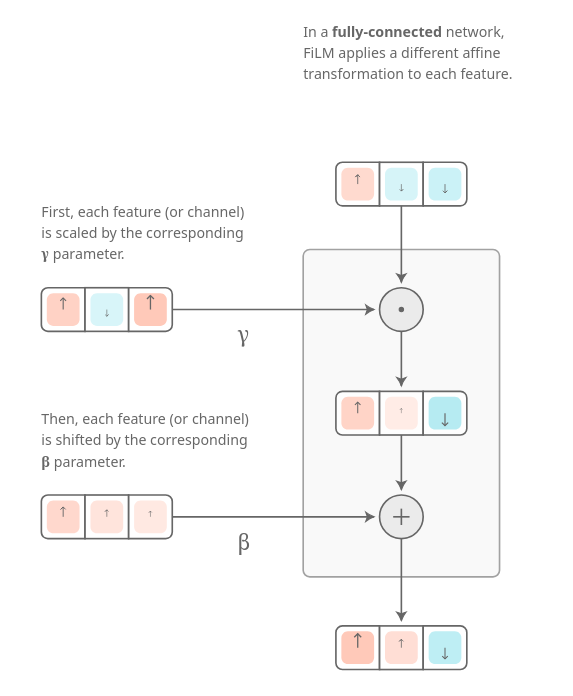
\includegraphics[width=0.5\textwidth]{film_layers.png}
    \caption{Illustration of the feature-wise transformation \cite{dumoulin2018feature-wise}}
    \label{fig:film}
\end{figure}

In our approach, we have attempted to decouple the perturbation effect, creating a perturbation free latent space, while taking control of the perturbation response with the conditioning vector. Thus, our architecture is based on an autoencoder, and the conditioning of the task, which in our case is the type of perturbation, will be delegated via FiLM layers fused in the decoder (\verb|MultiTaskAutoencoder|). The $\gamma$ and $\beta$ are designed to be different for each fusion.
% add a diagram here
We have experimented with a few variations of this, keeping the architecture of the decoder with the inclusion of film layers consistent. Thus, we have the following models:

\begin{itemize}
    \item The \verb|NultiTakAae| is based on an adversarial autoencoder. The discriminator aims to differentiate between control and perturbed gene expressions, and the encoder is trained to fool the discriminator.
    \item The \verb|MultiTaskAaeGaussian| is based on an adversarial autoencoder, that aims to create a latent space that follows the gaussian distribution. The discriminator aims to differentiate between samples of the gene expressions and the gaussian distribution.
    \item add the rest
\end{itemize}


\section{Evaluation}

To evaluate the models, we have used the count of DEGs, along with the $R^2$ of all the DEGs and the top 100 most variable ones. To complement the evaluation, based on scPerturb, we have calculated a set of five distance metrics, to capture the wholeness of the differences between the expected and predicted perturbed gene expressions.

We have tested the models on two datasets, one where human peripheral blood mononuclear cells have been stimulated by IFN-b interferon, and a multi-perturbation dataset, where liver cells have been stimulated by multiple doses of tetrachlorodibenzo-p-dioxin (TCDD) in vivo.

Regarding the single perturbation response models, the scGen, scButterfly, scPreGAN, in the multi-perturbation dataset of ten dosages, we have trained a dedicated model for each dosage.

To address the randomness of the models, we have performed the experiments three times, with three different seeds 1, 2, 19193, and the metrics have been averaged across experiments.


\section{Results}

\subsection{Knowledge transfer}

which tasks and why they are important?

\subsection{TODO}

\begin{itemize}
    \item batch effect
    \item interpretability
    \item explainability
    \item integration with multiple omics
\end{itemize}

\section{Conclusions}

\section{Future work}


\chapter{Benchmarking}
\label{ch:chapter1}

\clearpage


\section{Datasets}

\subsection{Nault et al. 2022}

\begin{figure}[h]
    \centering
    \begin{subfigure}[t]{0.49\textwidth}
        \centering
        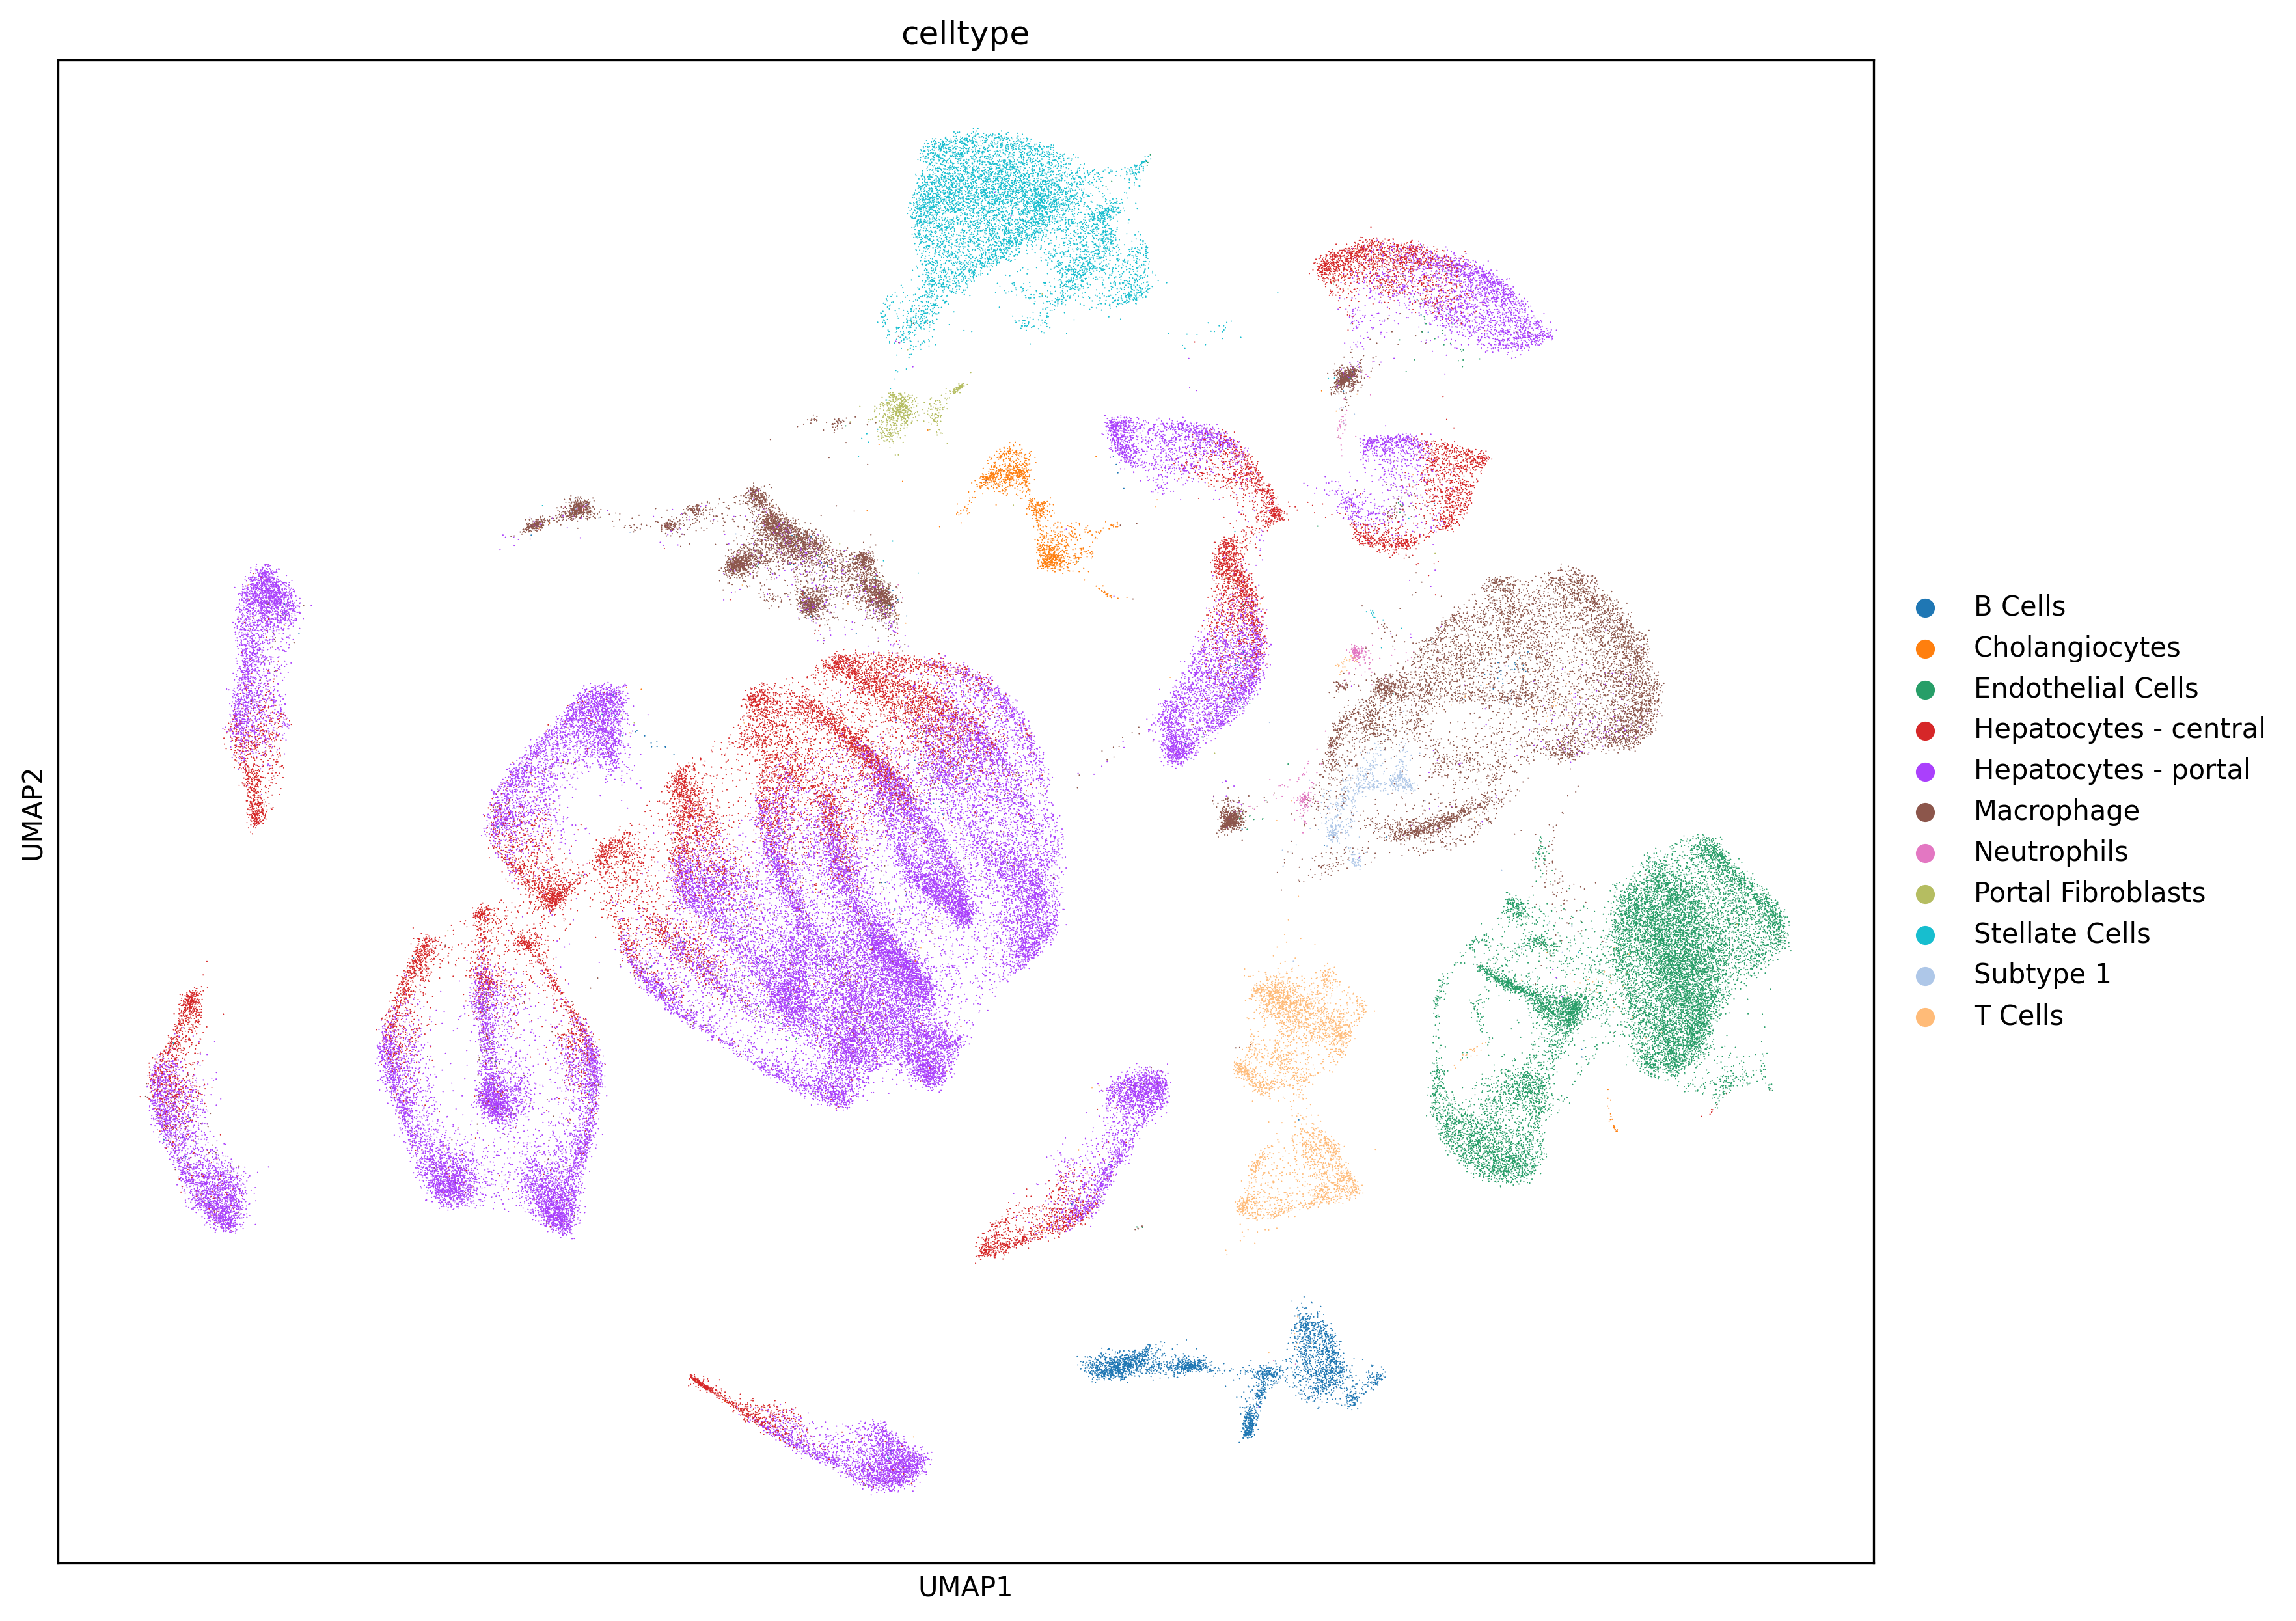
\includegraphics[width=.9\textwidth]{figures/nault_cell_umap.png}
        \caption{}
        \label{fig:figure1}.
    \end{subfigure}%
    \hfill
    \begin{subfigure}[t]{0.49\textwidth}
        \centering
        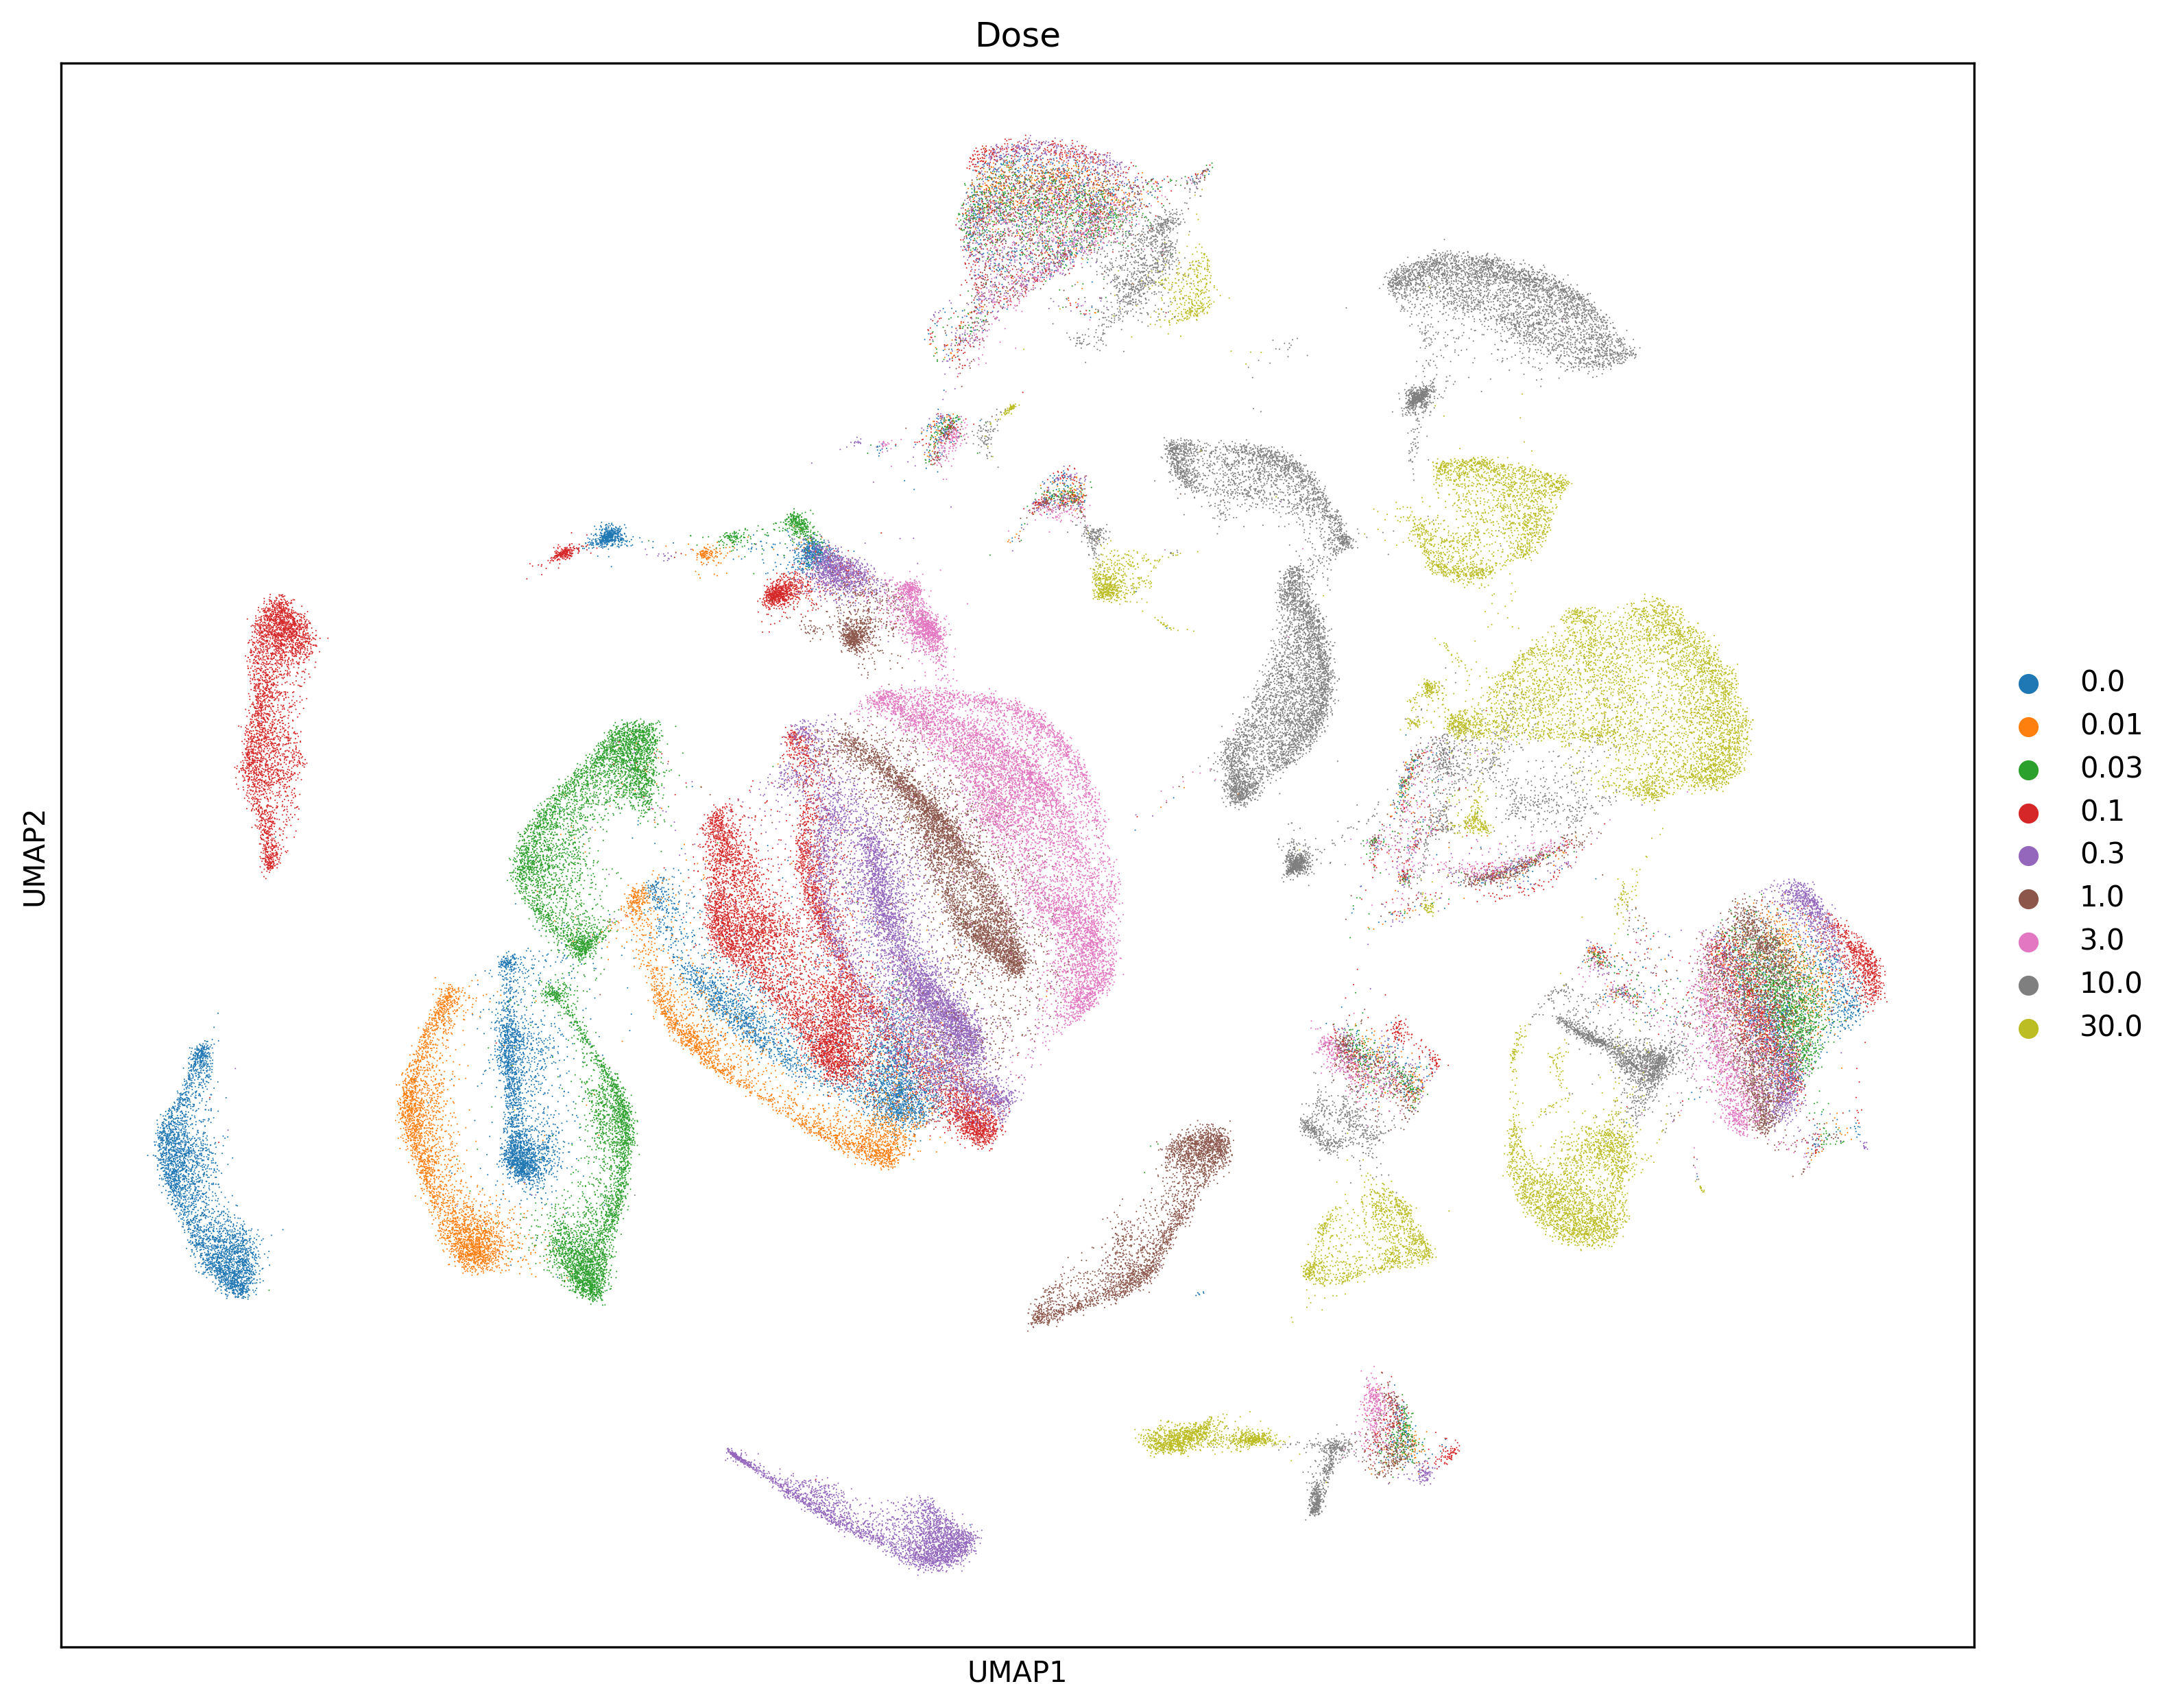
\includegraphics[width=.8\textwidth]{figures/nault_dose_umap.png}
        \caption{}
        \label{fig:figure2}
    \end{subfigure}%
    \hfill
    \begin{subfigure}[b]{\textwidth}
        \centering
        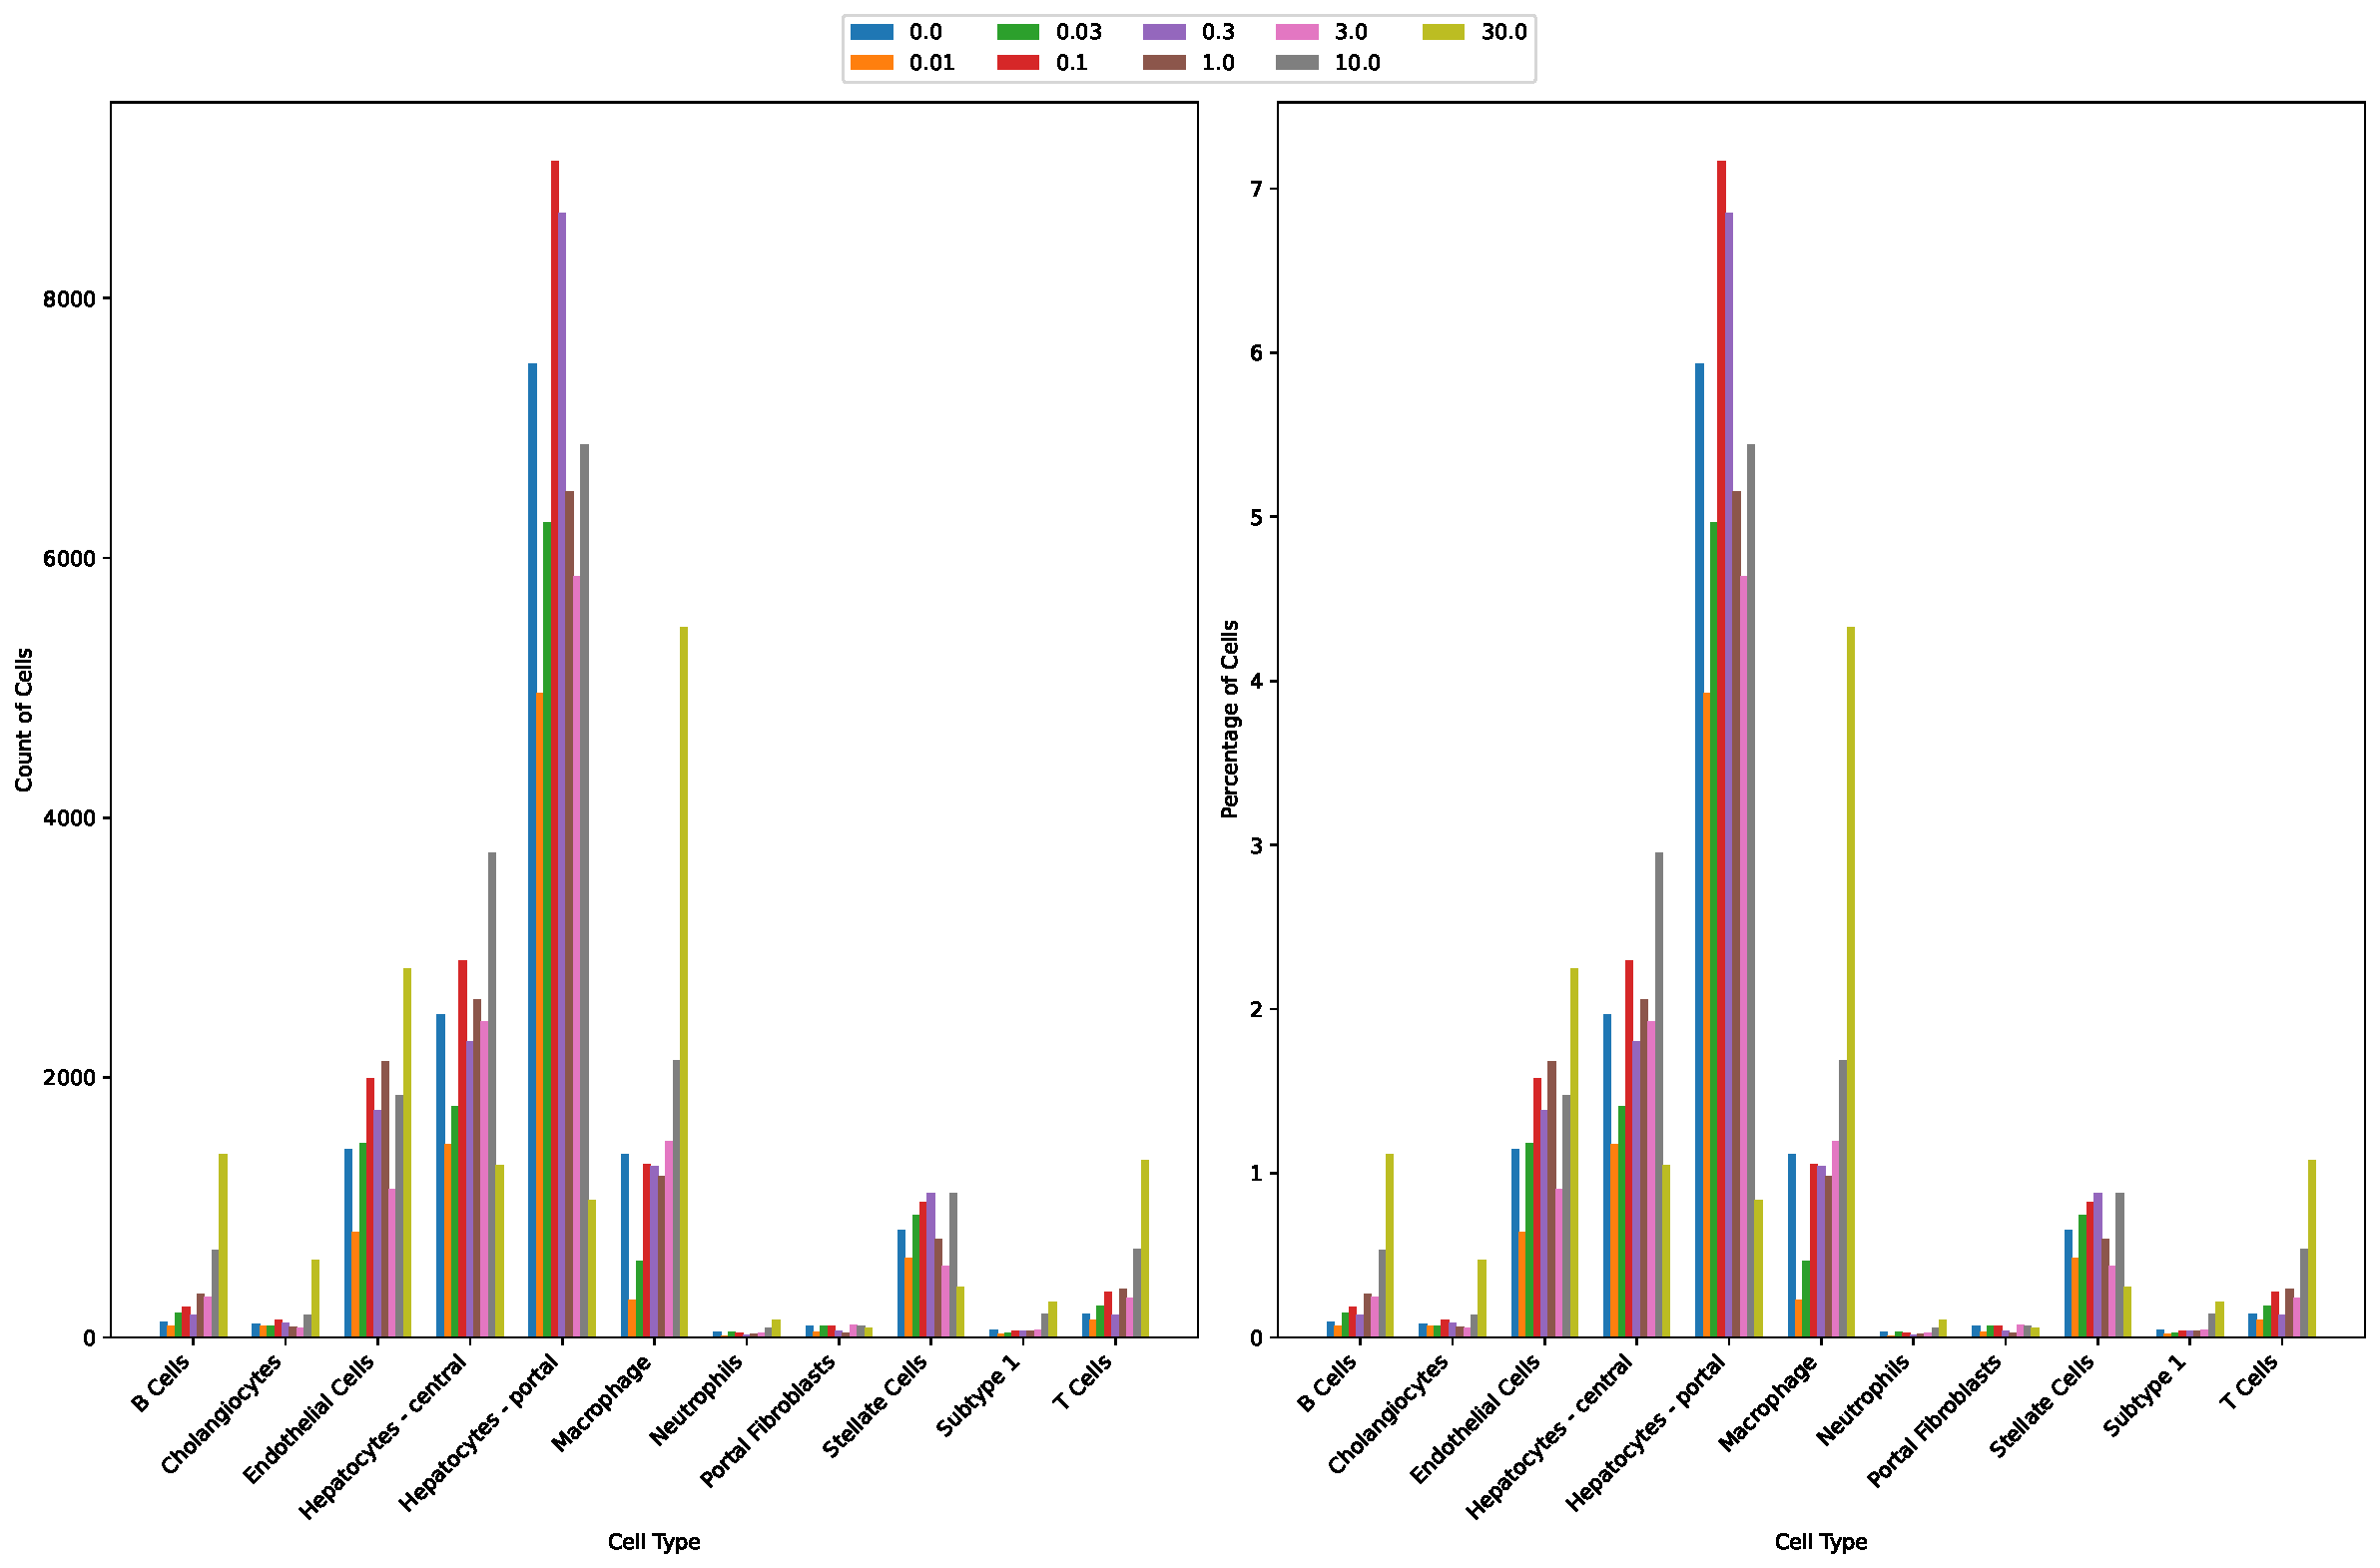
\includegraphics[width=.7\textwidth]{figures/nault_dosages_counts.pdf}
        \caption{}
        \label{fig:figure3}
    \end{subfigure}
    \hfill
    \begin{subfigure}[b]{\textwidth}
        \centering
        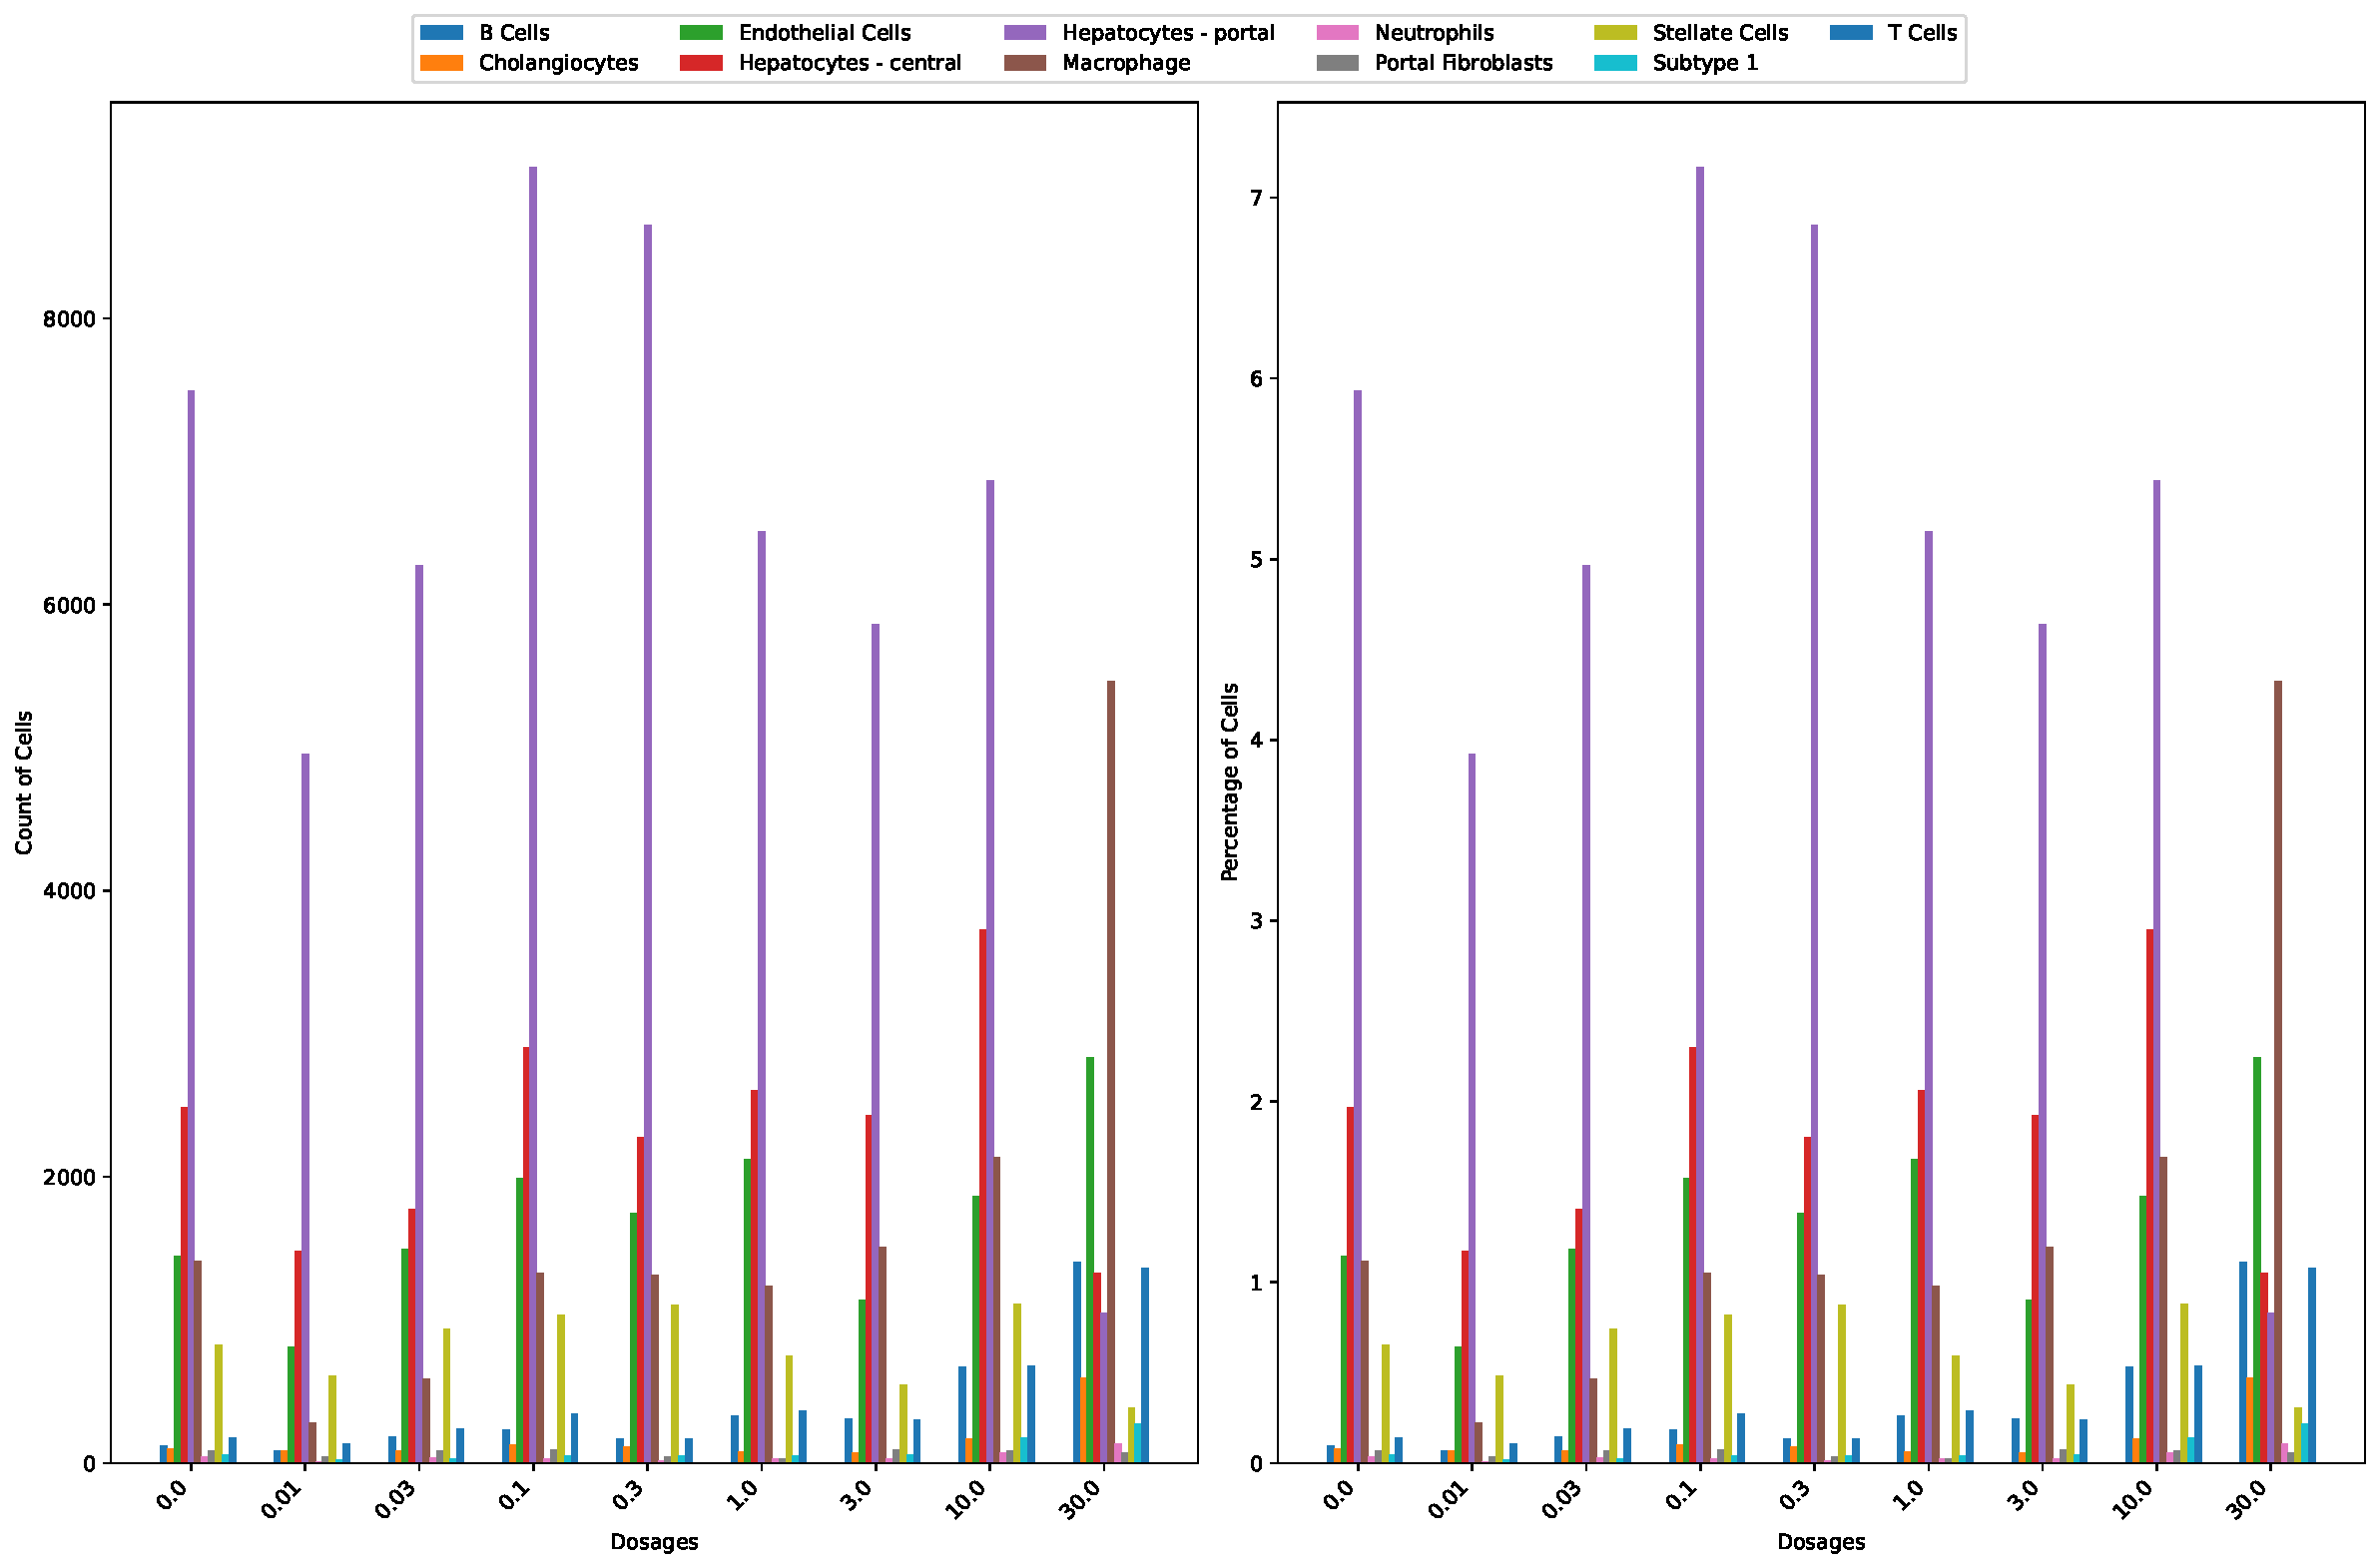
\includegraphics[width=.7\textwidth]{figures/nault_cell_types_counts.pdf}
        \caption{}
        \label{fig:figure4}
    \end{subfigure}    
    \caption{Nault overview}
    \label{fig:combined}
\end{figure}



\begin{figure}
    \centering
    \begin{minipage}{0.4\textwidth}
        \centering
        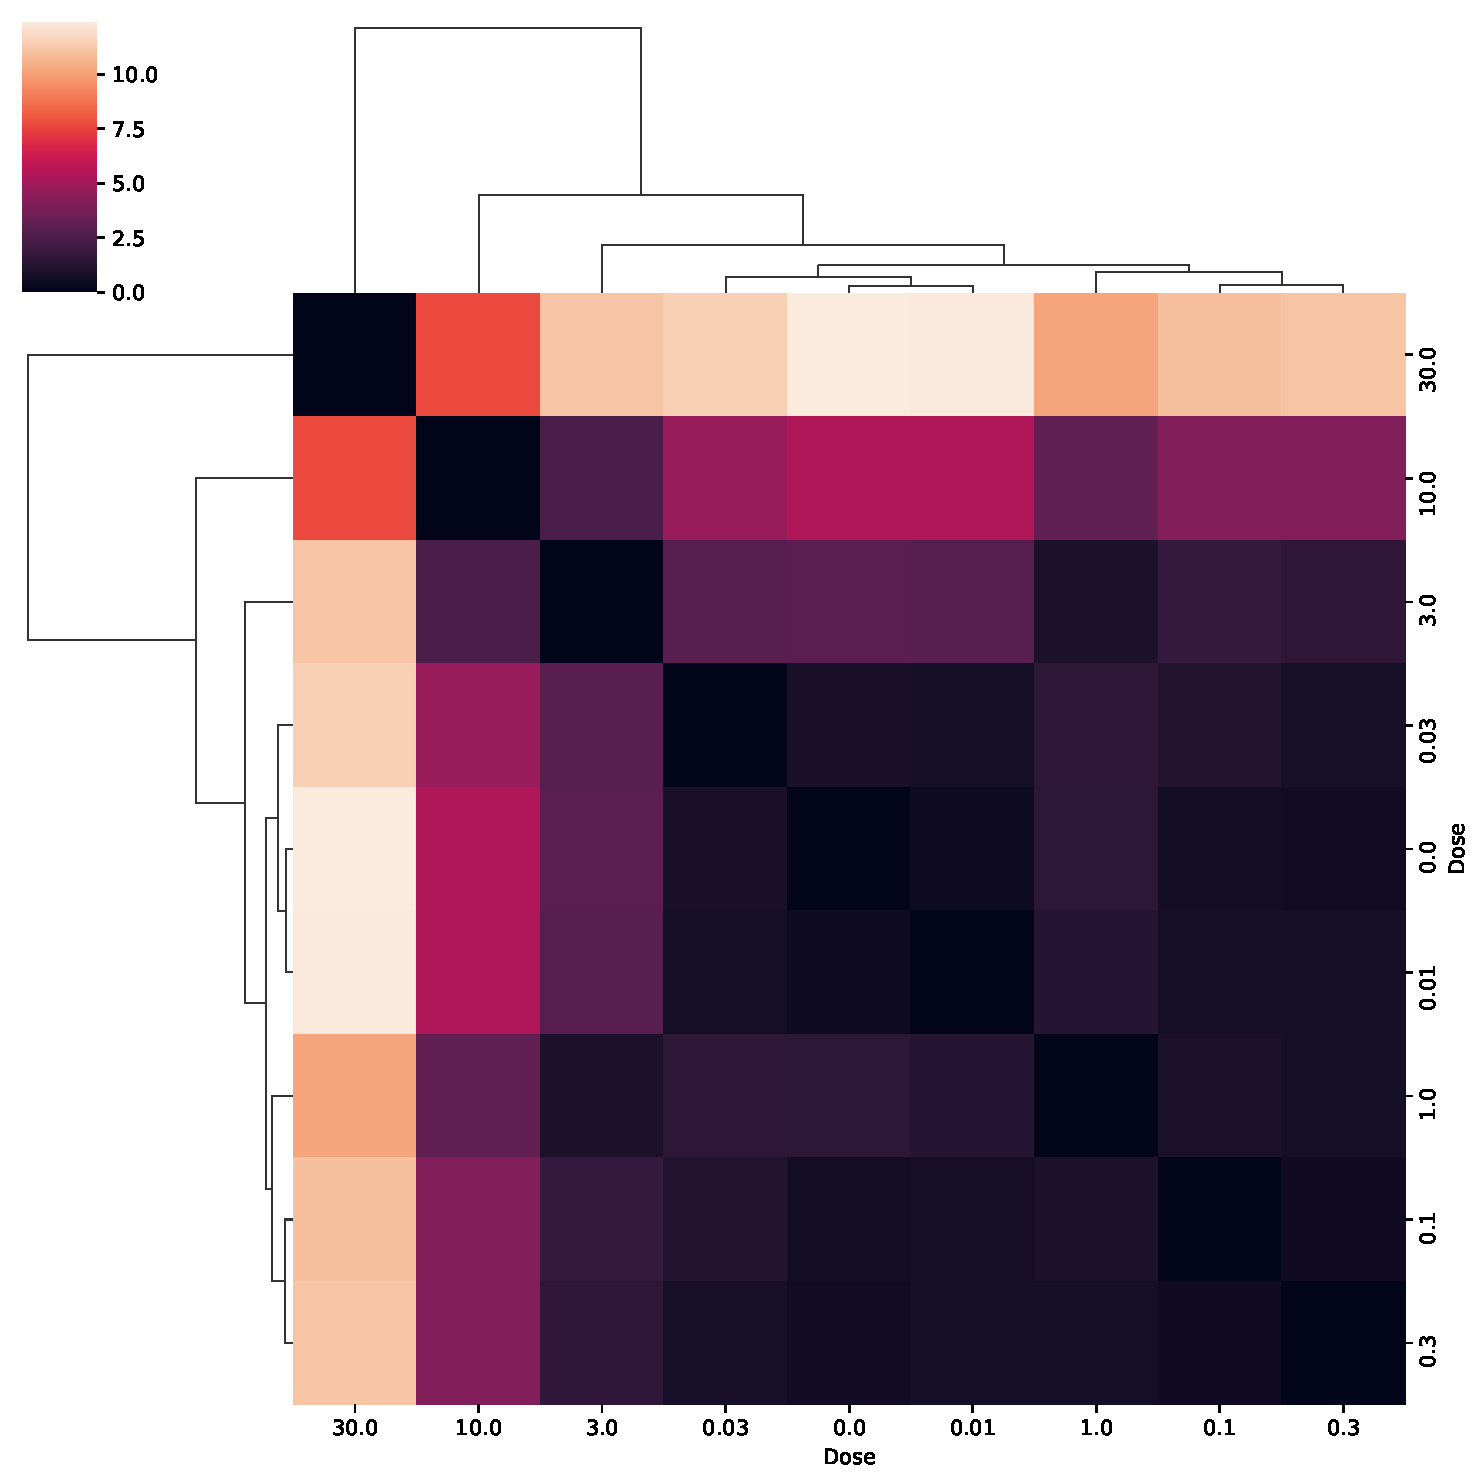
\includegraphics[width=\textwidth]{figures/nault_edistance_clustermap.pdf}
        \caption{E-distance}
    \end{minipage} \hfill
    \begin{minipage}{0.4\textwidth}
        \centering
        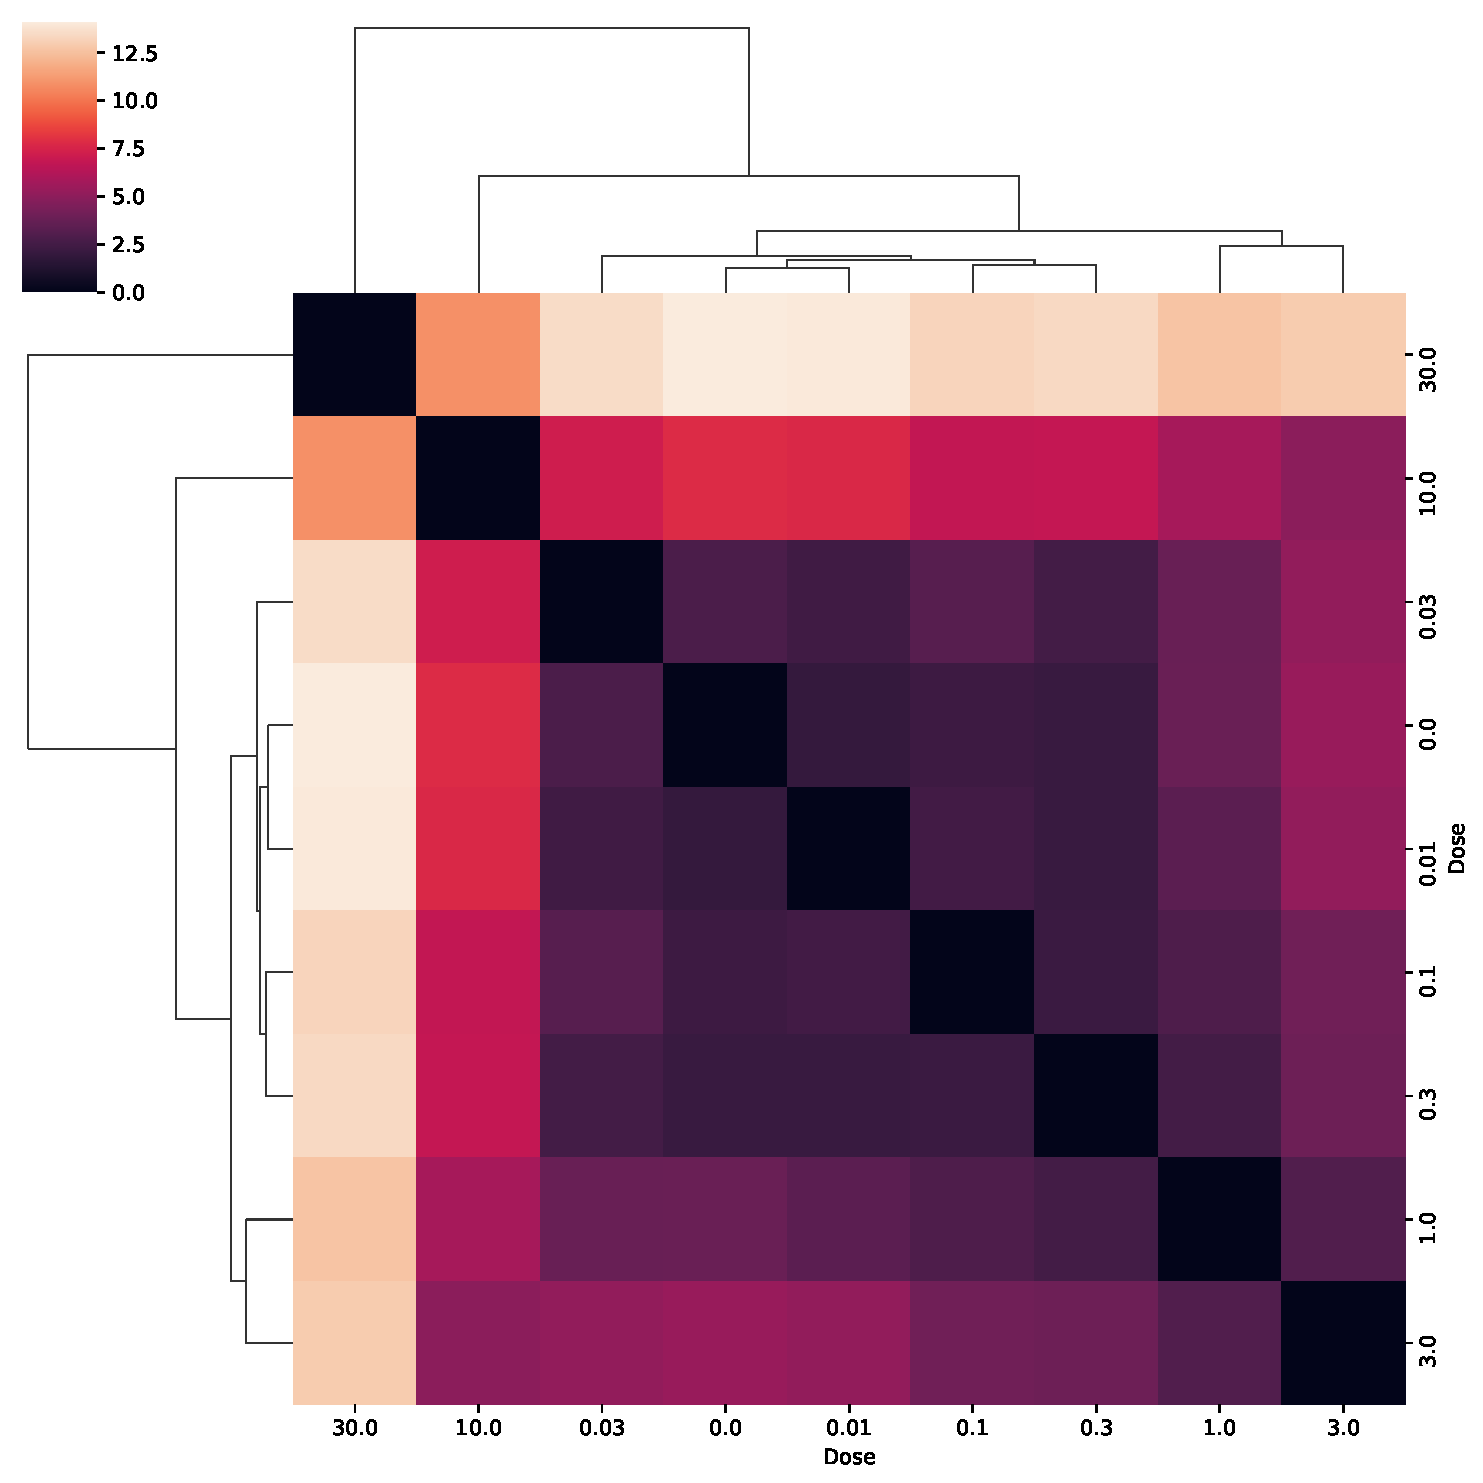
\includegraphics[width=\textwidth]{figures/nault_euclidean_clustermap.pdf}
        \caption{Euclidean}
    \end{minipage}
    \vskip\baselineskip

    \begin{minipage}{0.4\textwidth}
        \centering
        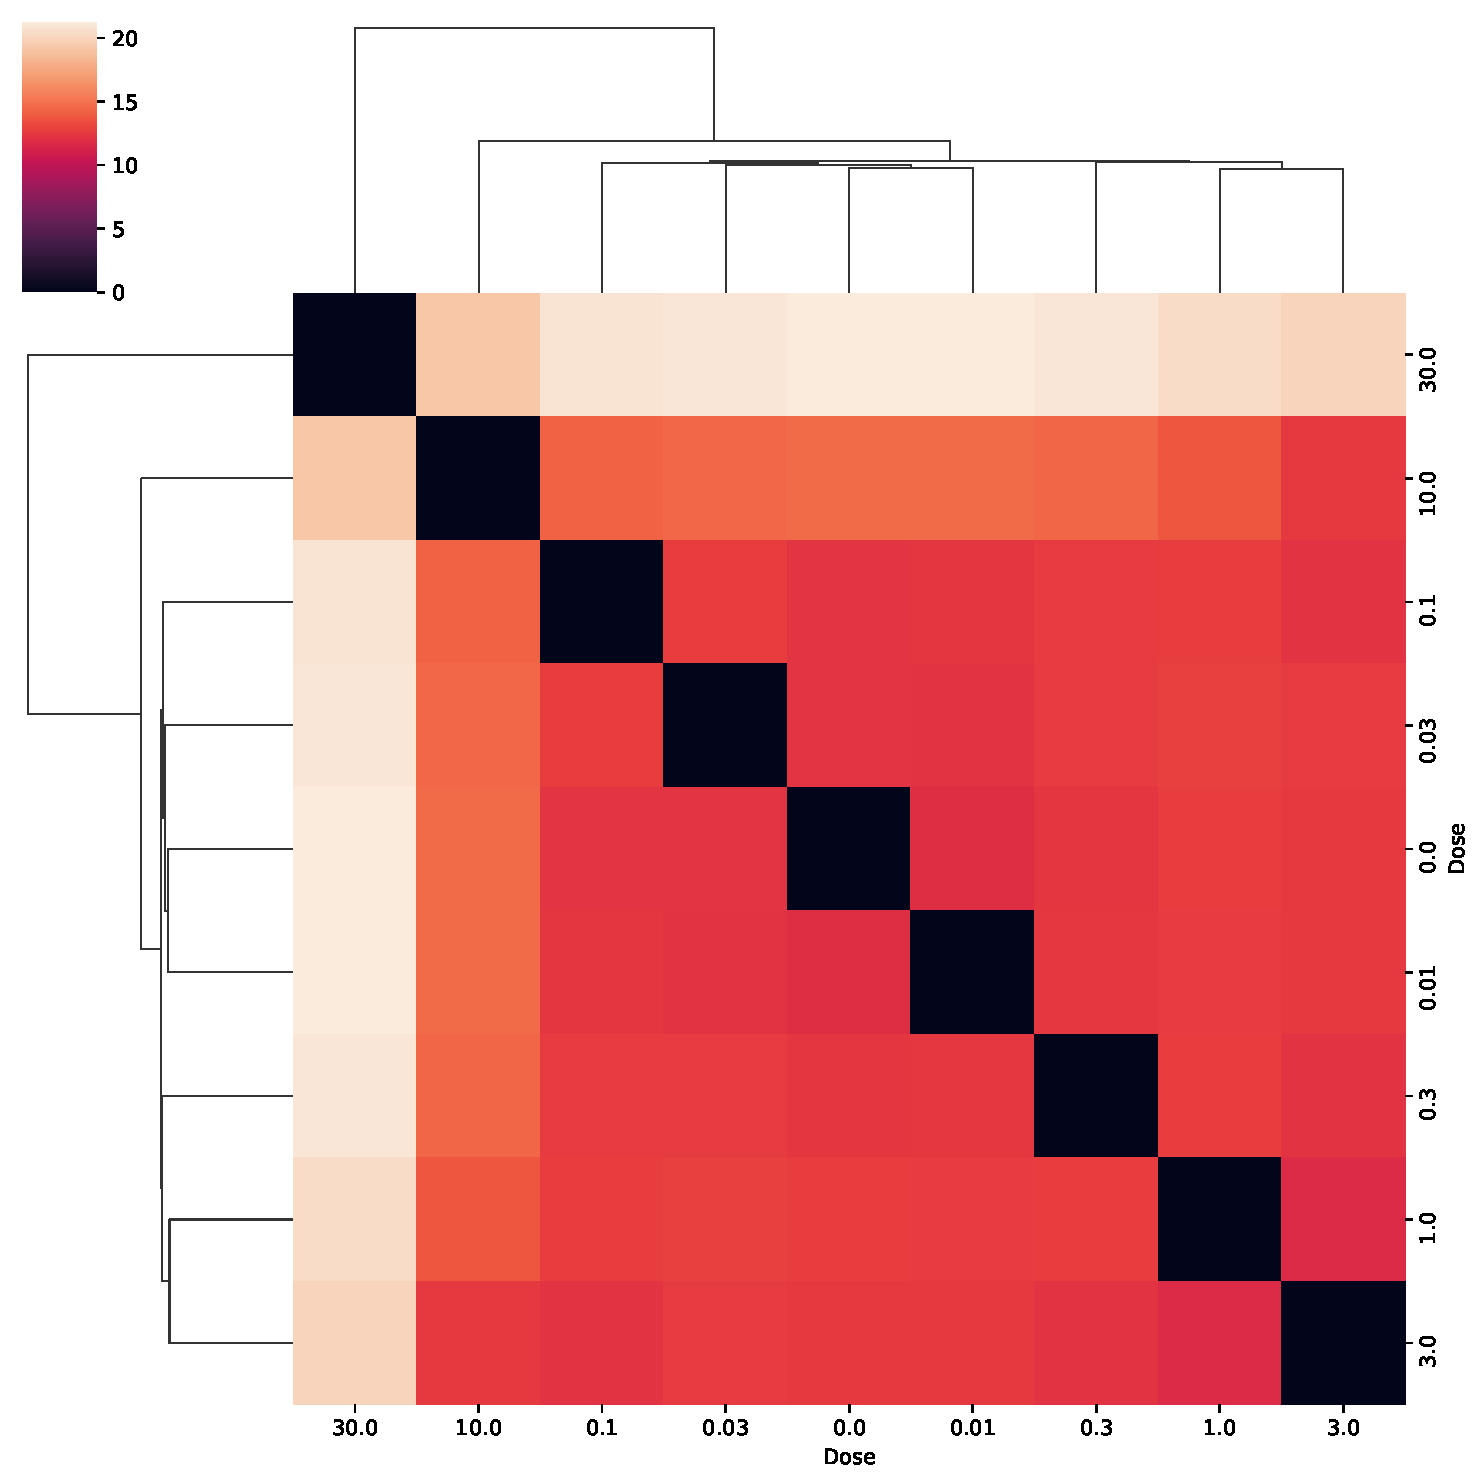
\includegraphics[width=\textwidth]{figures/nault_mean_pairwise_clustermap.pdf}
        \caption{Mean pairwise}
    \end{minipage} \hfill
    \begin{minipage}{0.4\textwidth}
        \centering
        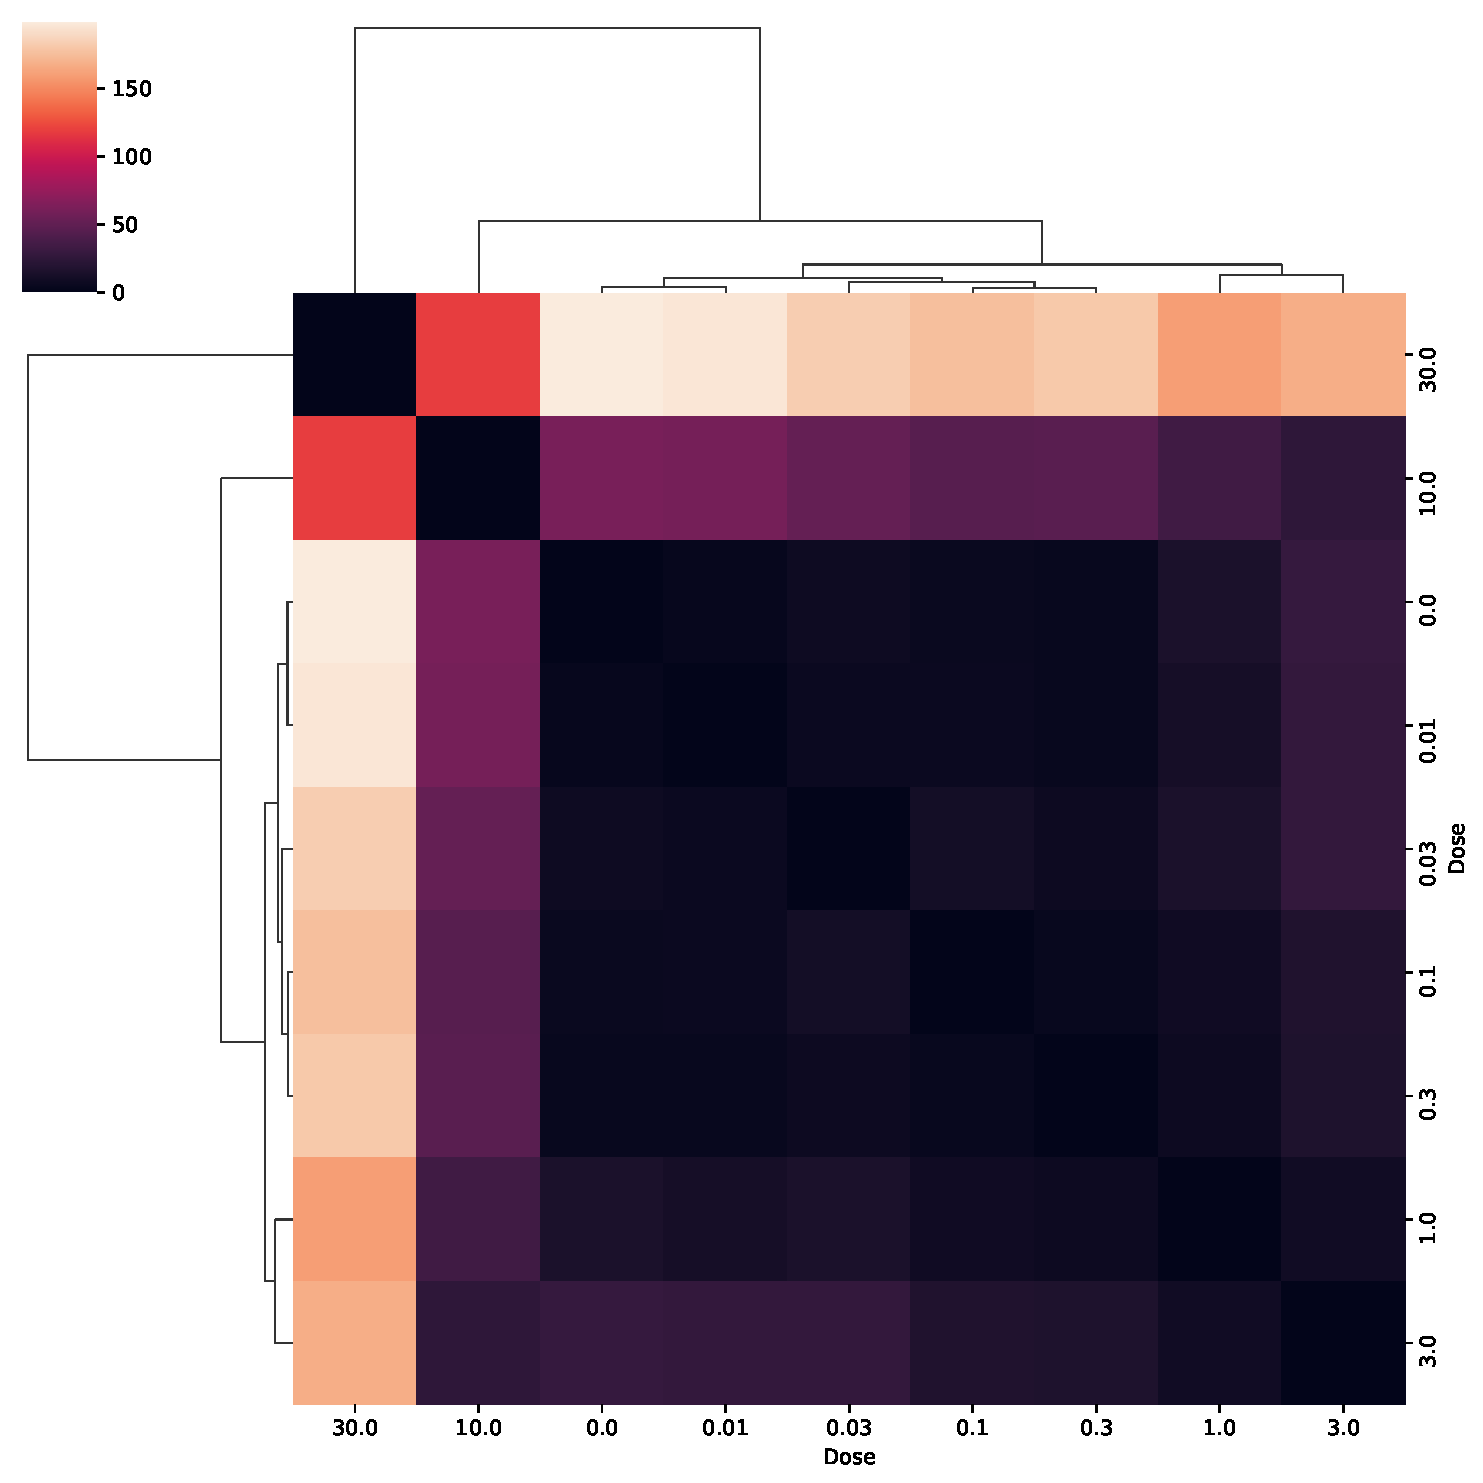
\includegraphics[width=\textwidth]{figures/nault_mmd_clustermap.pdf}
        \caption{MMD}
    \end{minipage}
    \vskip\baselineskip

    \begin{minipage}{0.4\textwidth}
        \centering
        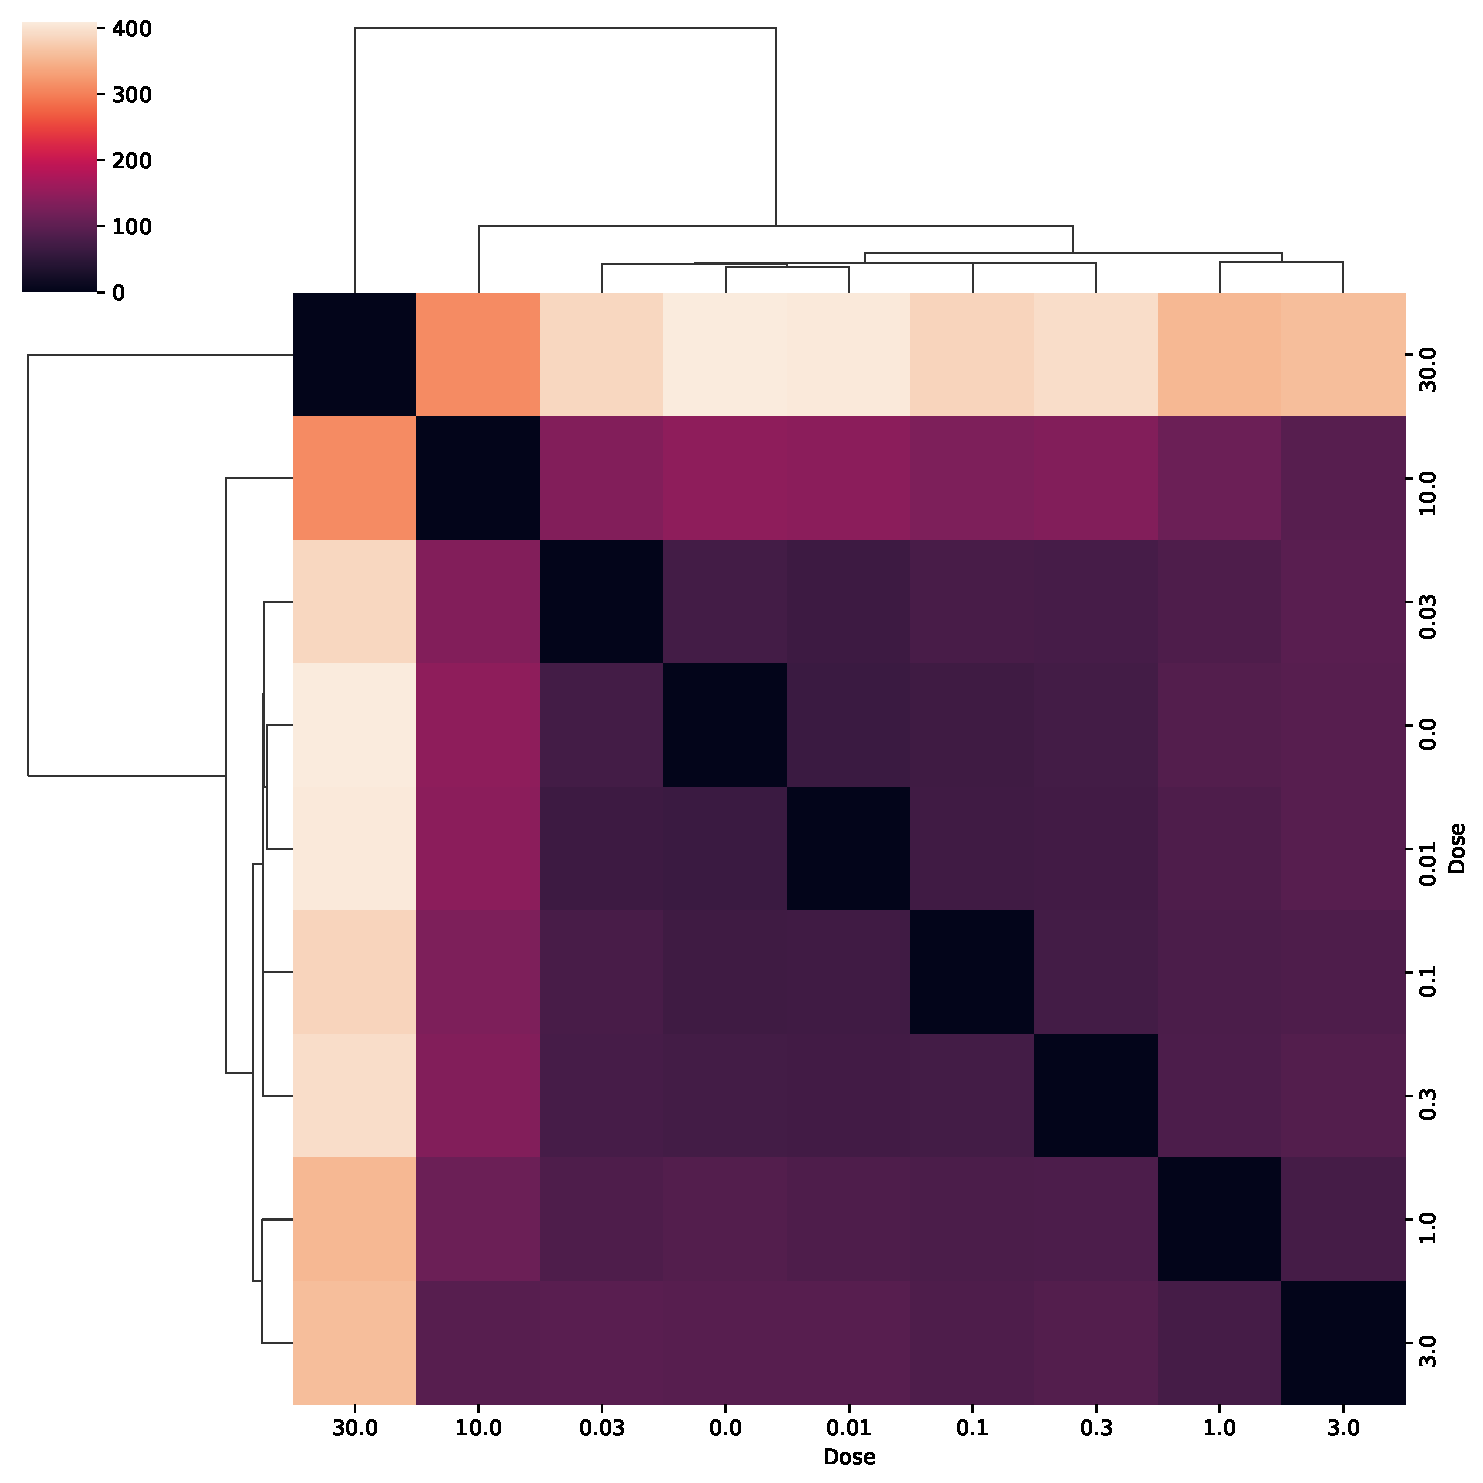
\includegraphics[width=\textwidth]{figures/nault_wasserstein_clustermap.pdf}
        \caption{Wasserstein}
    \end{minipage}
    \caption{Distance metrics across all cell types per dosage}
\end{figure}

\begin{figure}
    \centering
    \begin{minipage}{0.4\textwidth}
        \centering
        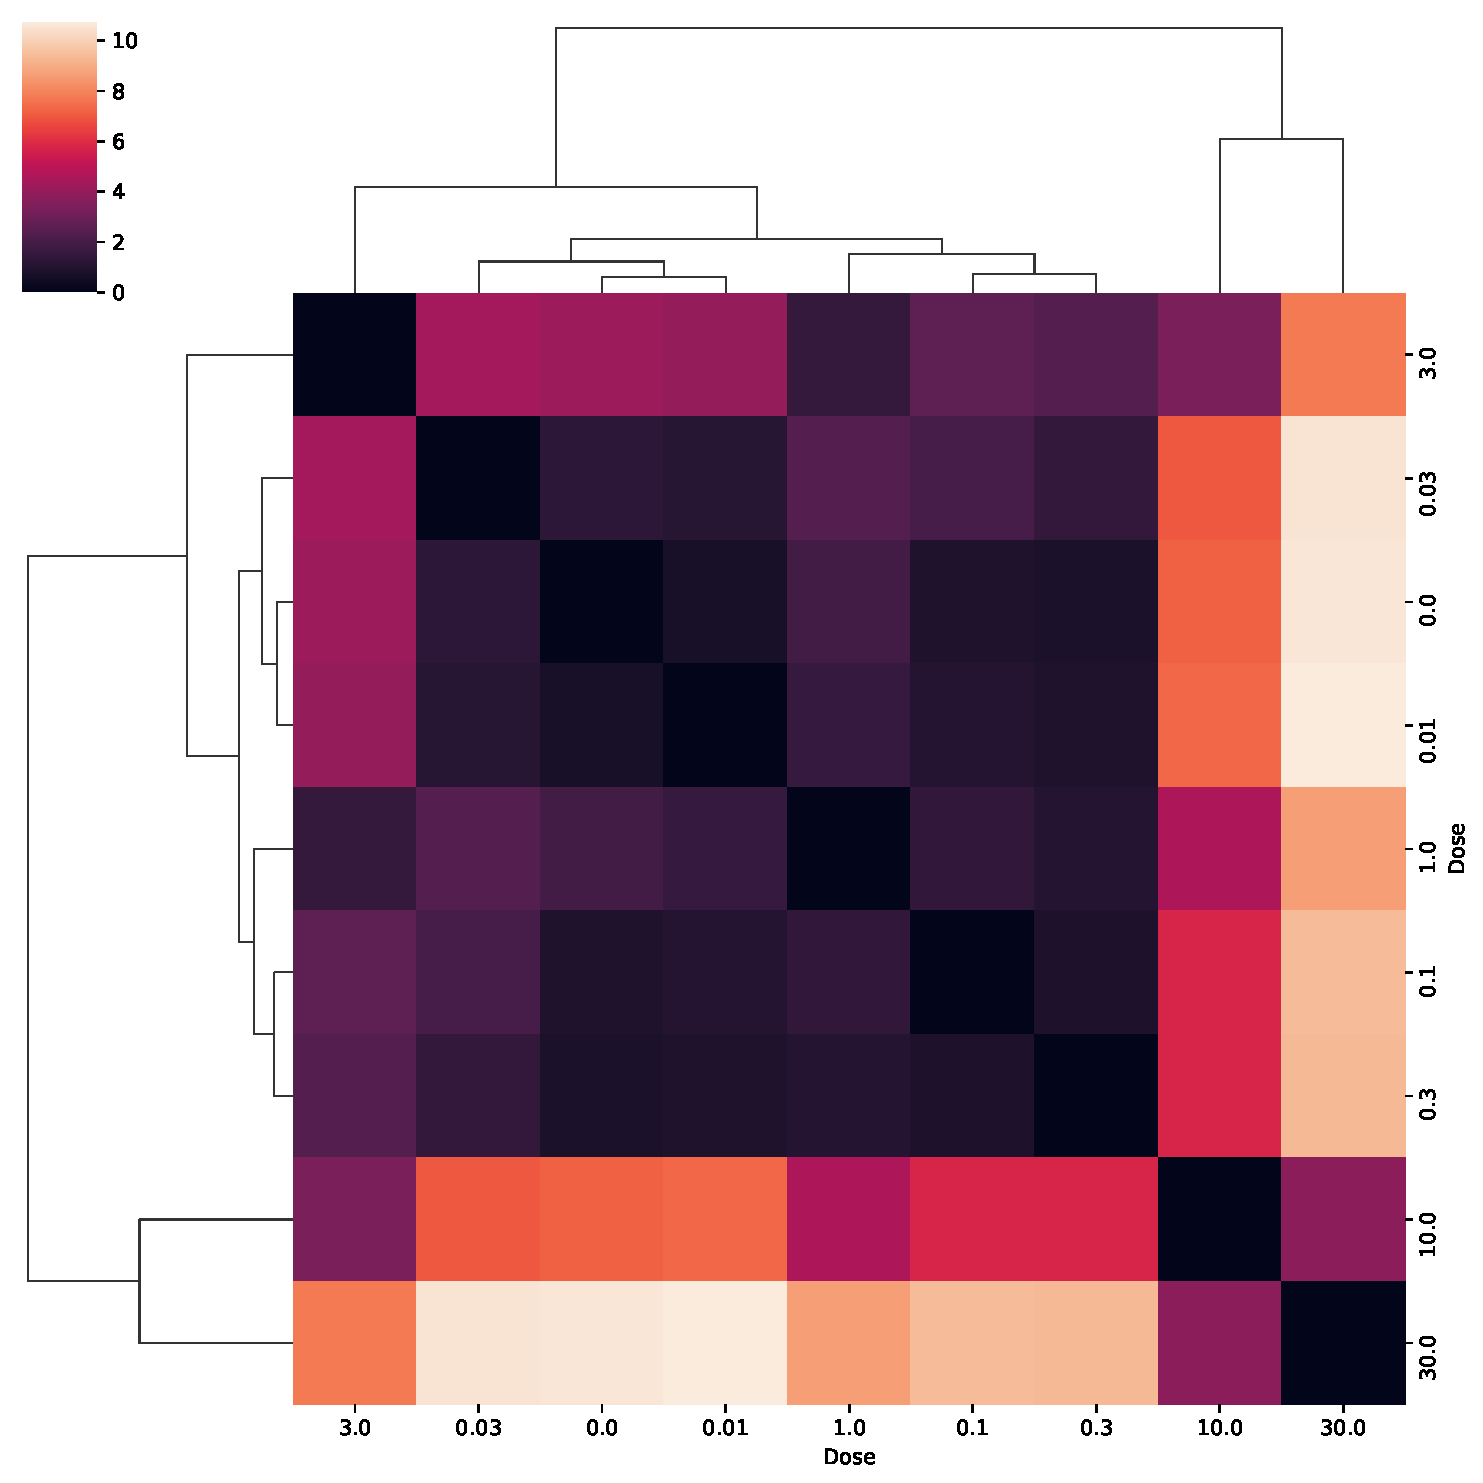
\includegraphics[width=\textwidth]{figures/hepatocytes_edistance_clustermap.pdf}
        \caption{E-distance}
    \end{minipage} \hfill
    \begin{minipage}{0.4\textwidth}
        \centering
        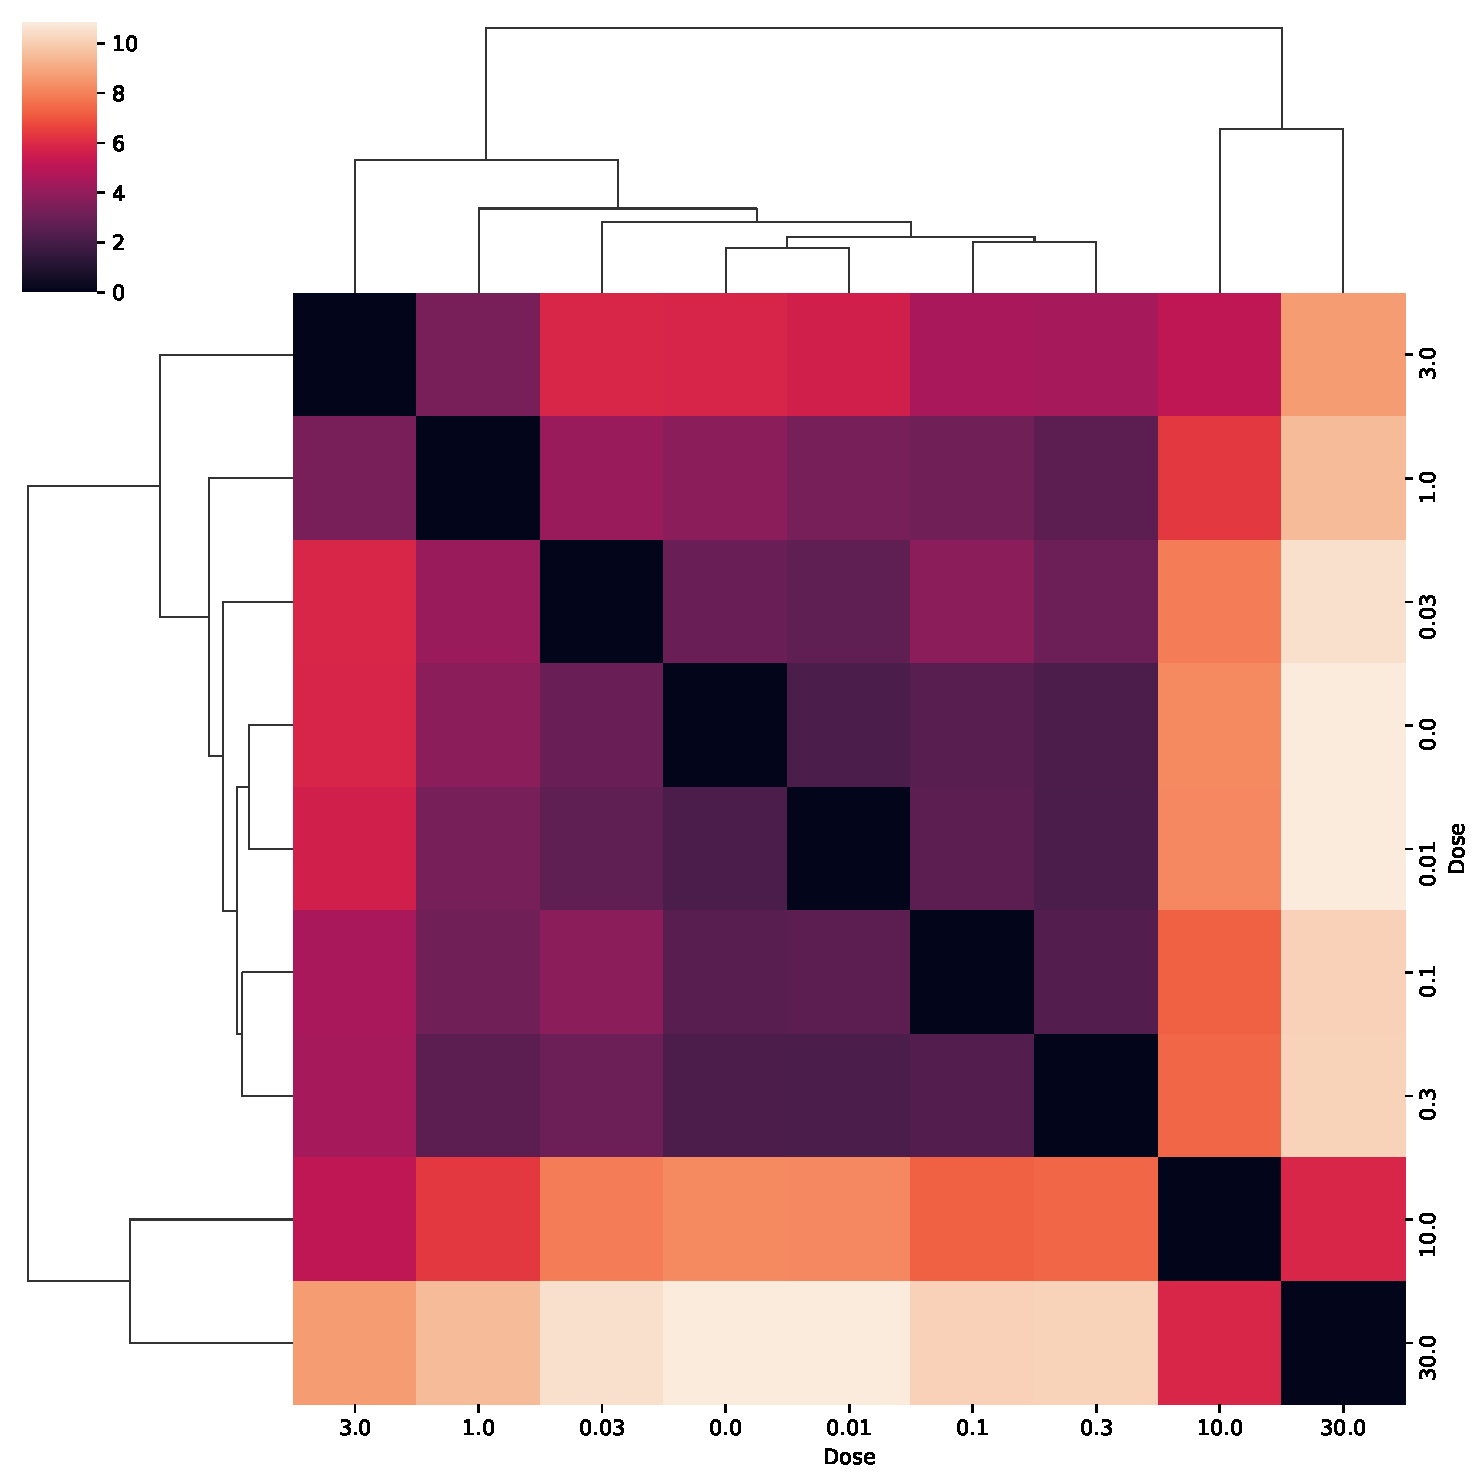
\includegraphics[width=\textwidth]{figures/hepatocytes_euclidean_clustermap.pdf}
        \caption{Euclidean}
    \end{minipage}
    \vskip\baselineskip

    \begin{minipage}{0.4\textwidth}
        \centering
        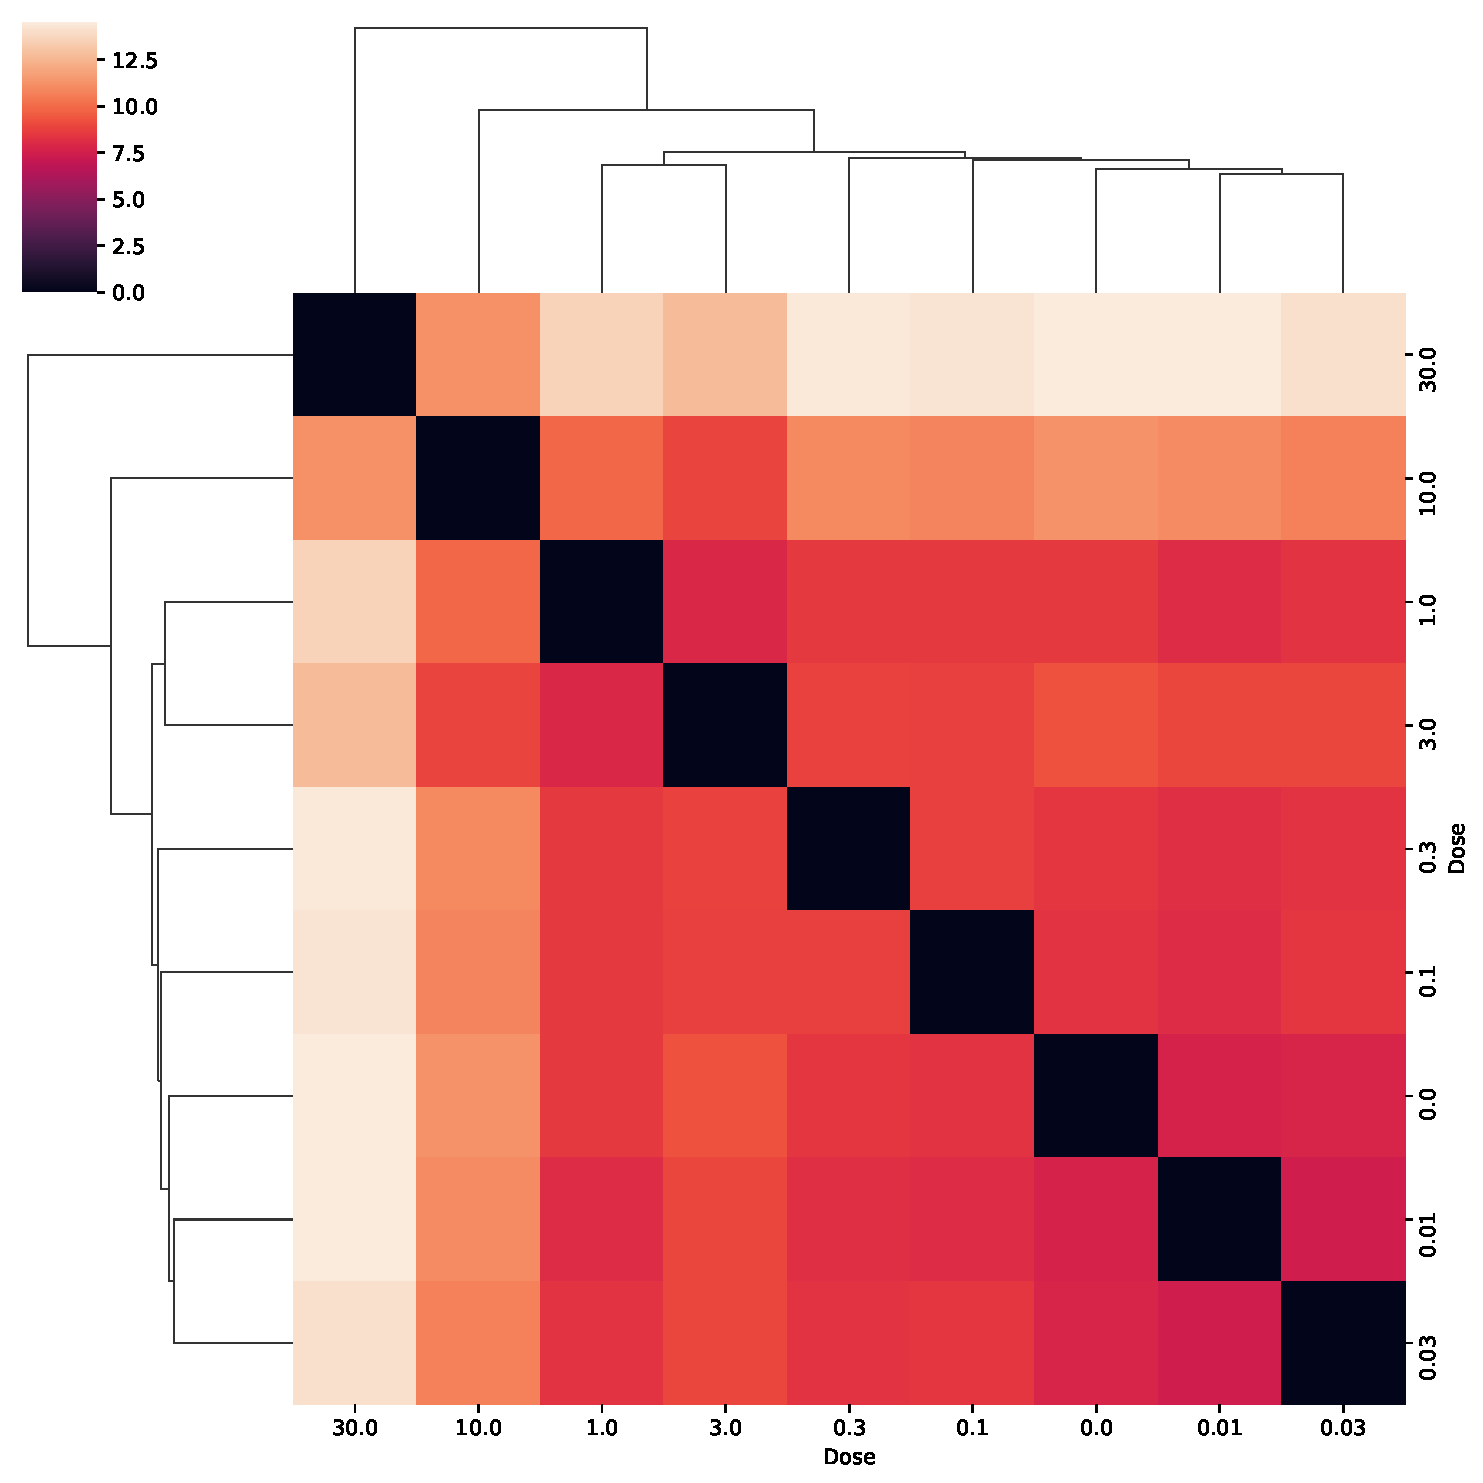
\includegraphics[width=\textwidth]{figures/hepatocytes_mean_pairwise_clustermap.pdf}
        \caption{Mean pairwise}
    \end{minipage} \hfill
    \begin{minipage}{0.4\textwidth}
        \centering
        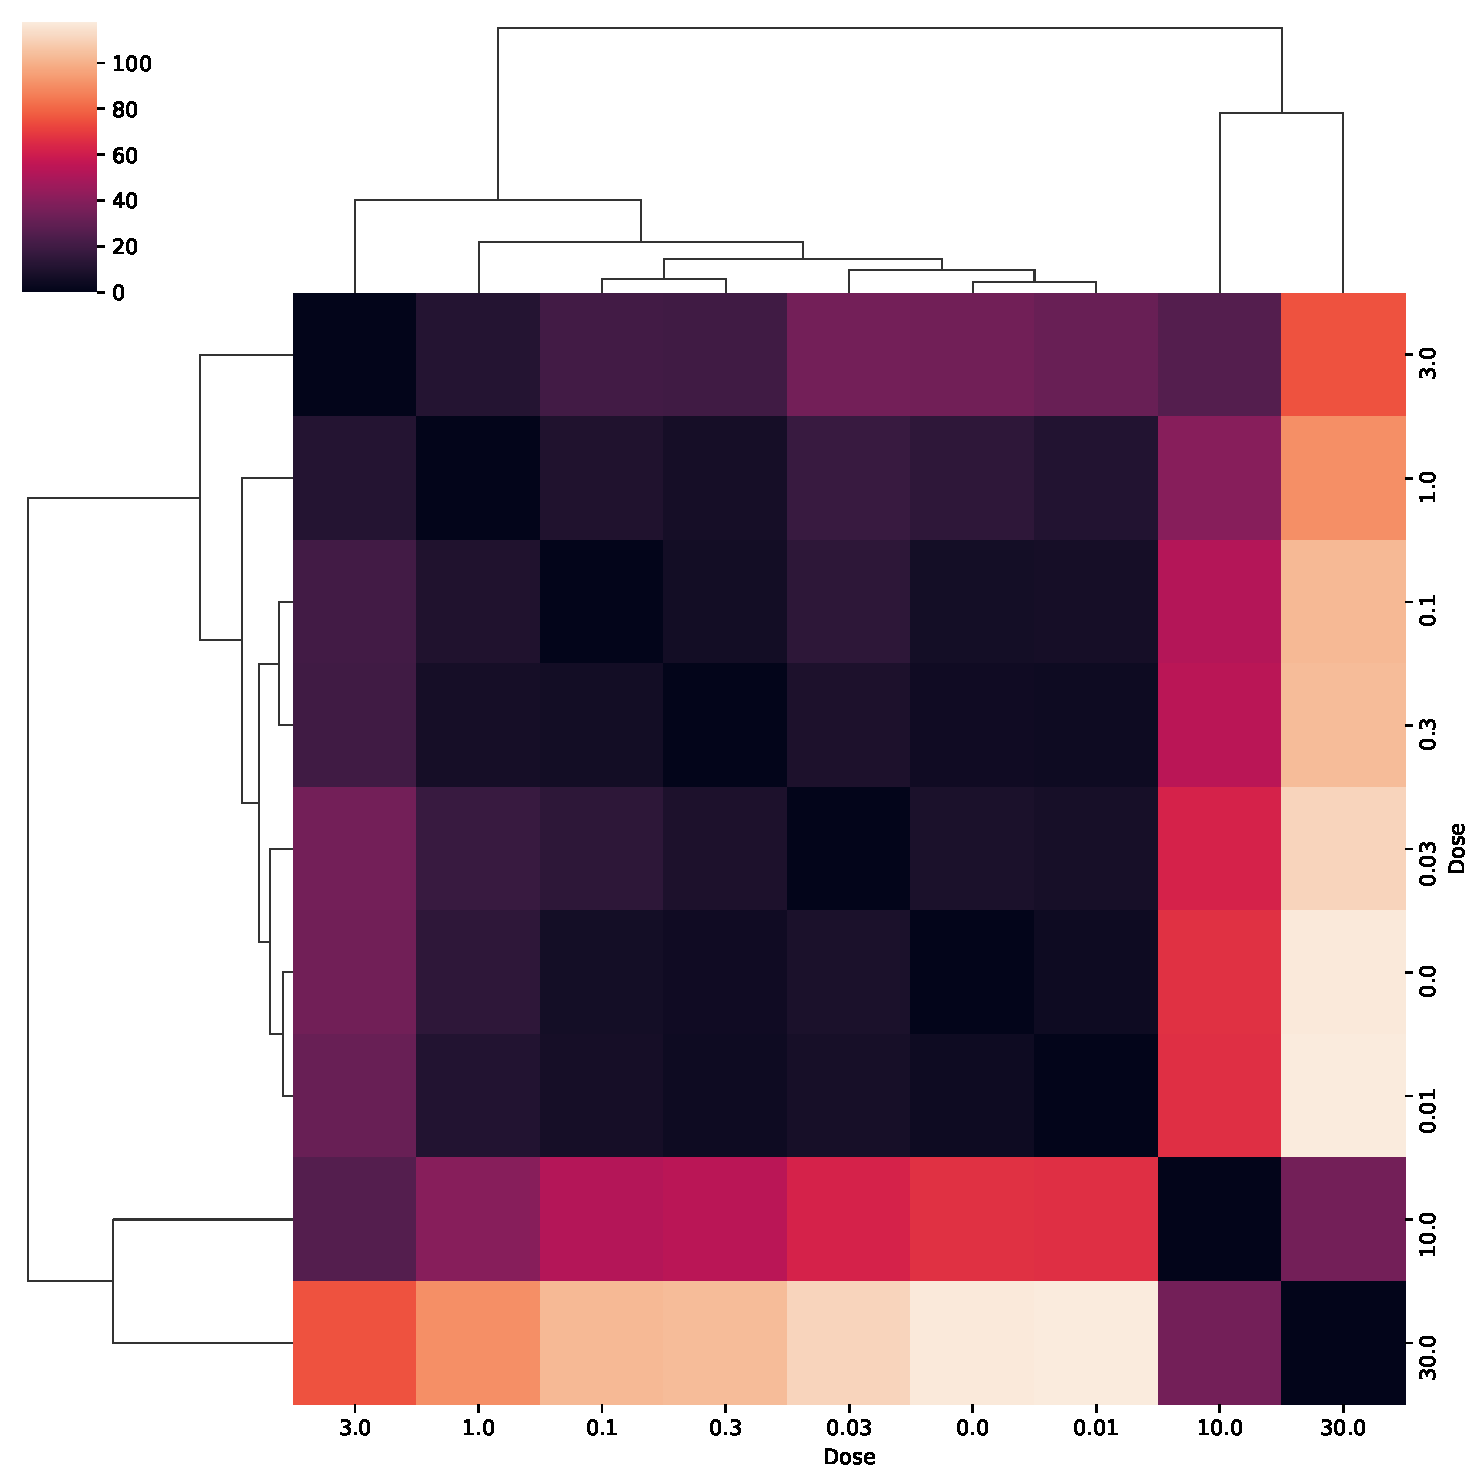
\includegraphics[width=\textwidth]{figures/hepatocytes_mmd_clustermap.pdf}
        \caption{MMD}
    \end{minipage}
    \vskip\baselineskip

    \begin{minipage}{0.4\textwidth}
        \centering
        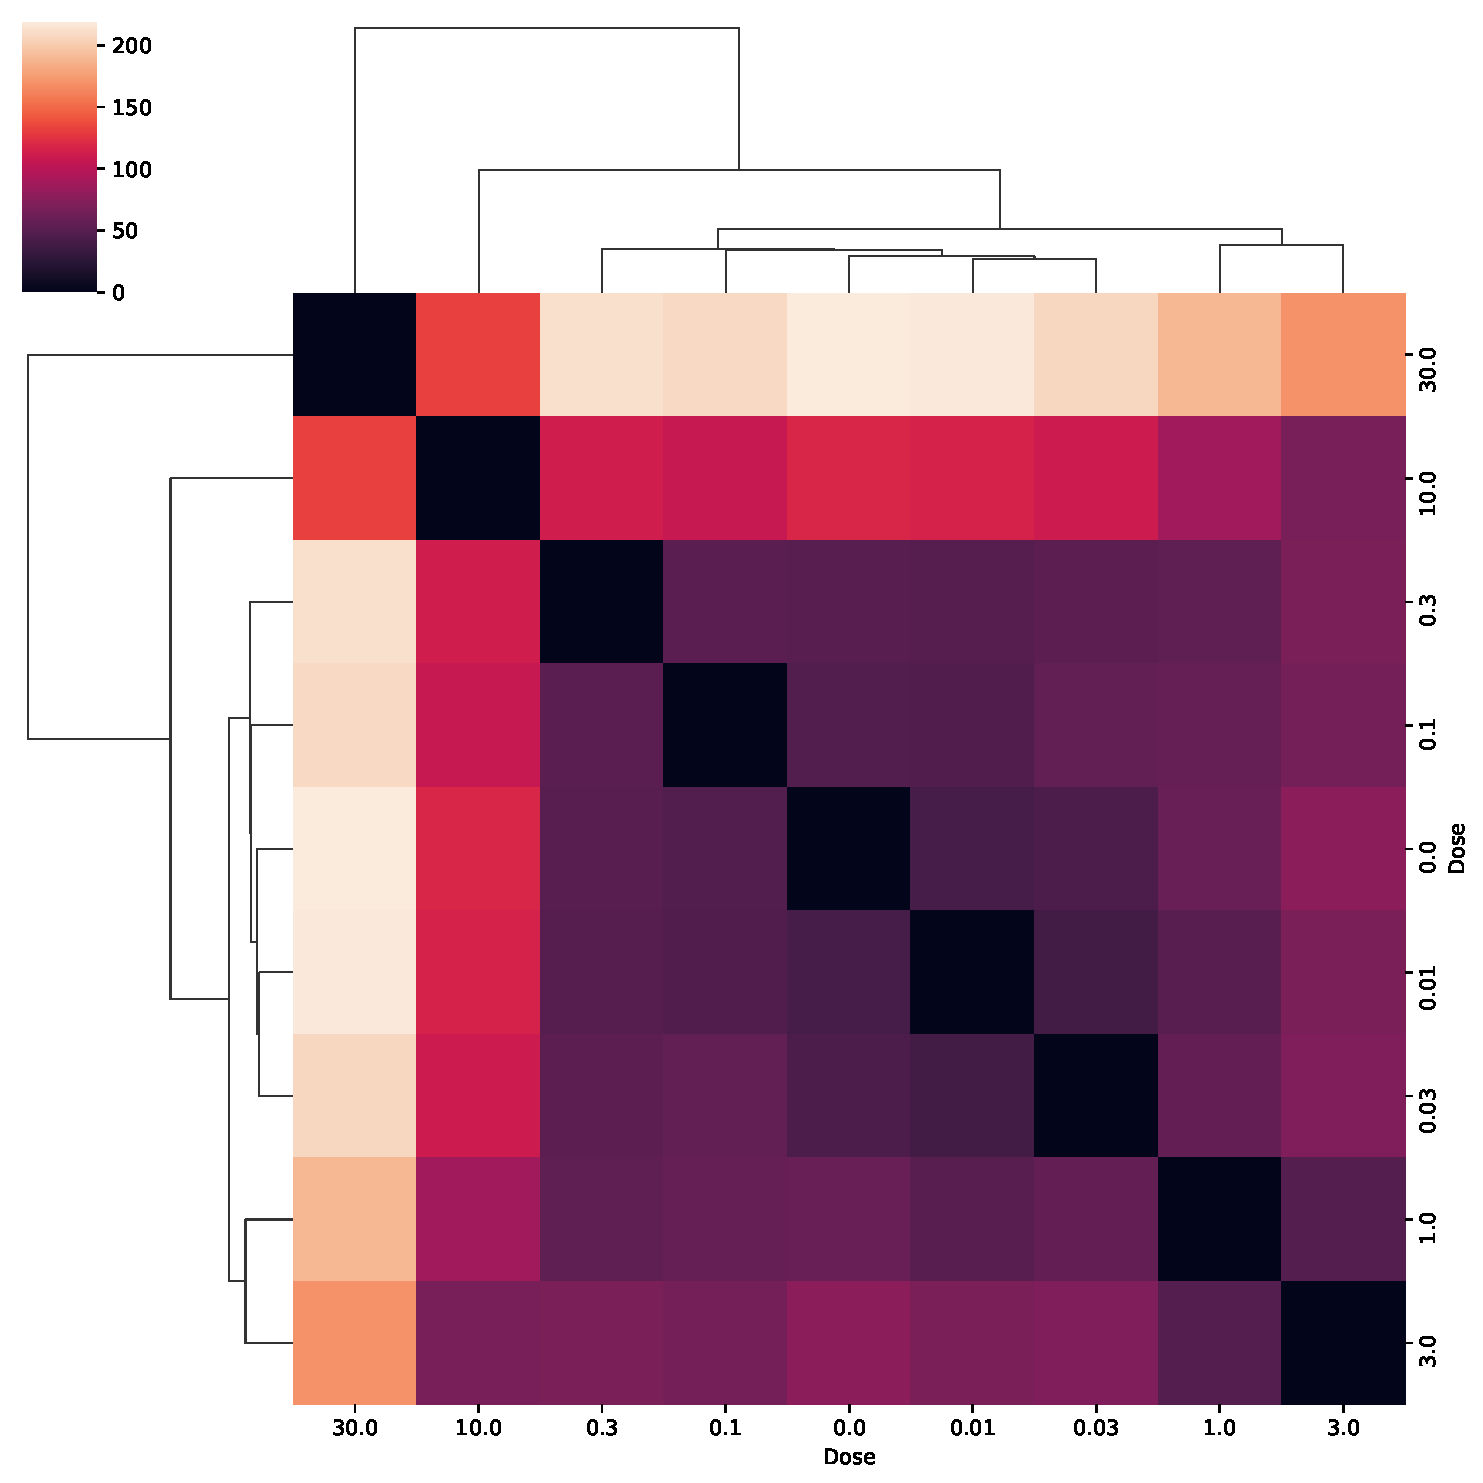
\includegraphics[width=\textwidth]{figures/hepatocytes_wasserstein_clustermap.pdf}
        \caption{Wasserstein}
    \end{minipage}
    \caption{Distance metrics for cell type Hepatocytes - portal per dosage}
\end{figure}

\begin{figure}
    \centering
    \begin{minipage}{0.4\textwidth}
        \centering
        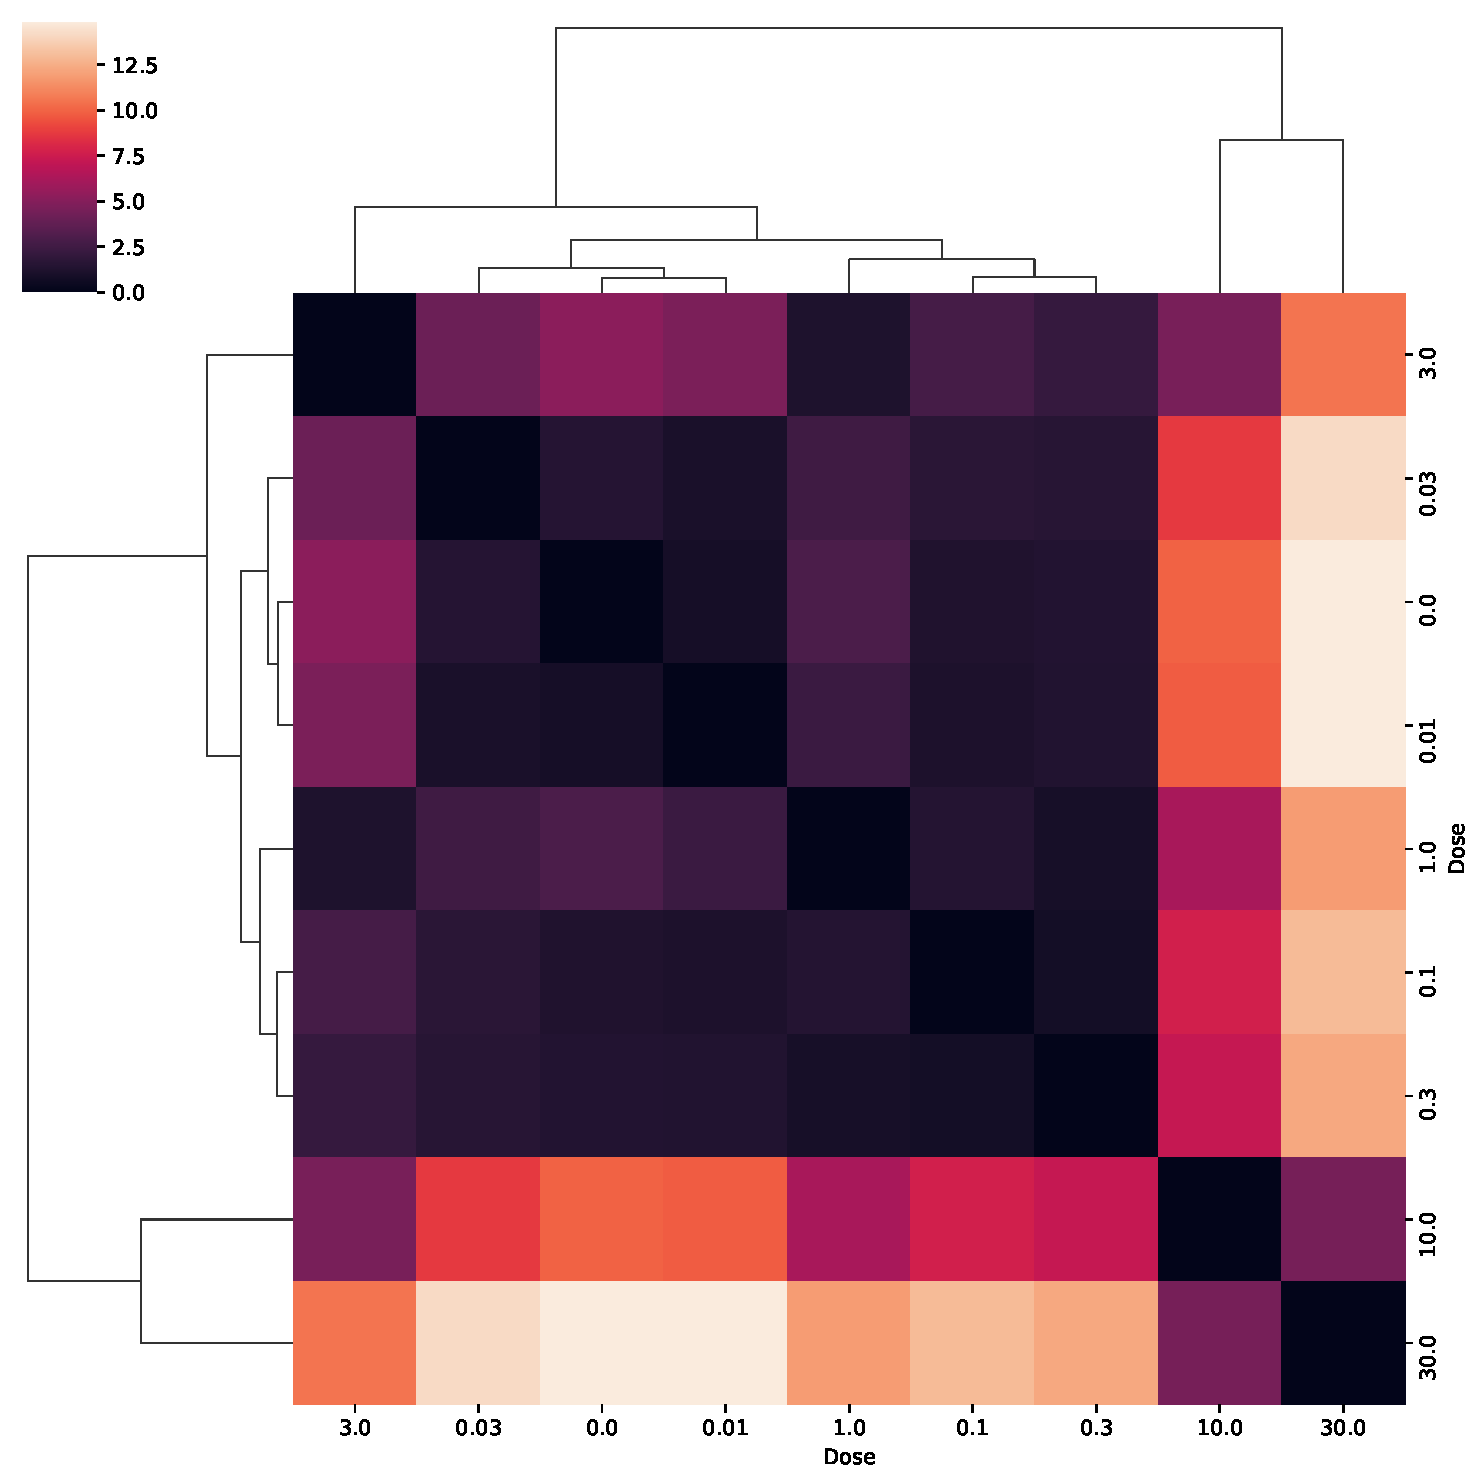
\includegraphics[width=\textwidth]{figures/hepatocytes_central_edistance_clustermap.pdf}
        \caption{E-distance}
    \end{minipage} \hfill
    \begin{minipage}{0.4\textwidth}
        \centering
        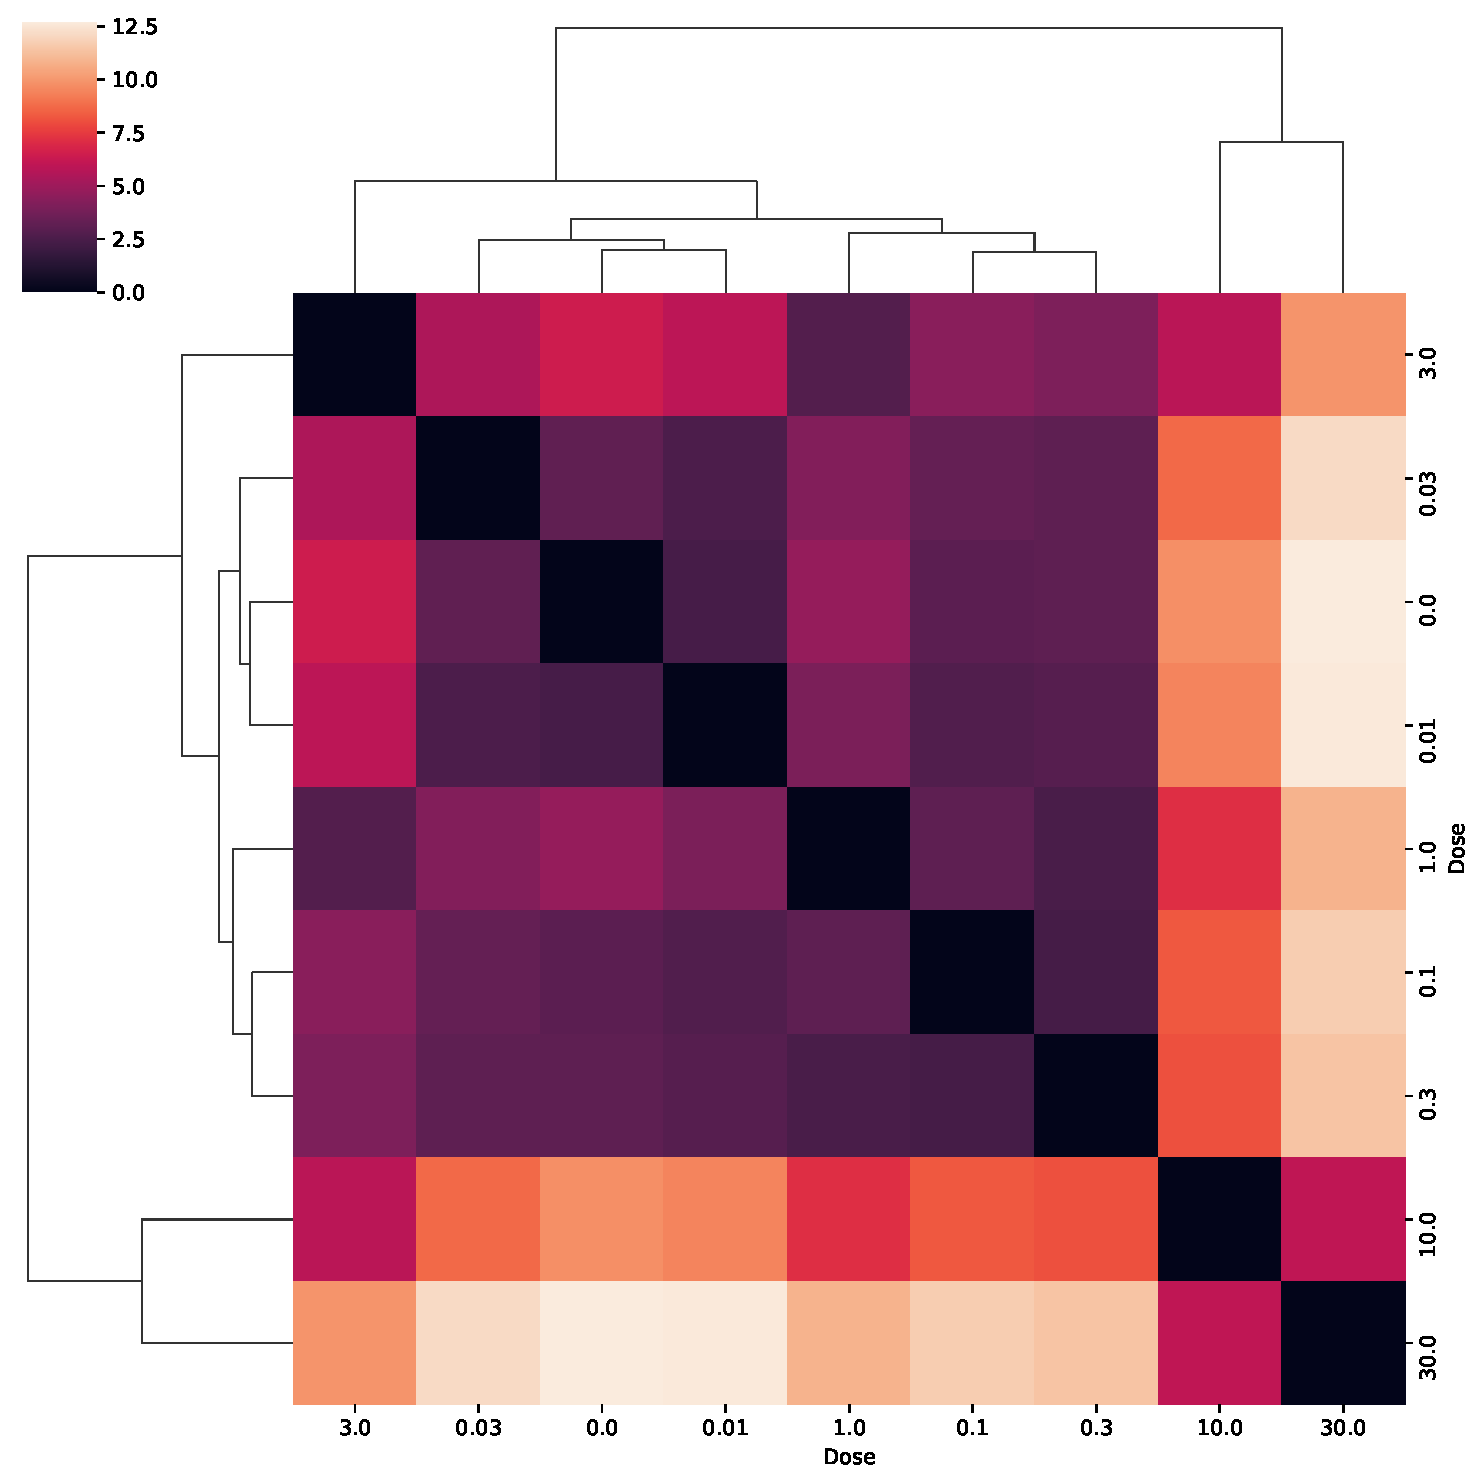
\includegraphics[width=\textwidth]{figures/hepatocytes_central_euclidean_clustermap.pdf}
        \caption{Euclidean}
    \end{minipage}
    \vskip\baselineskip

    \begin{minipage}{0.4\textwidth}
        \centering
        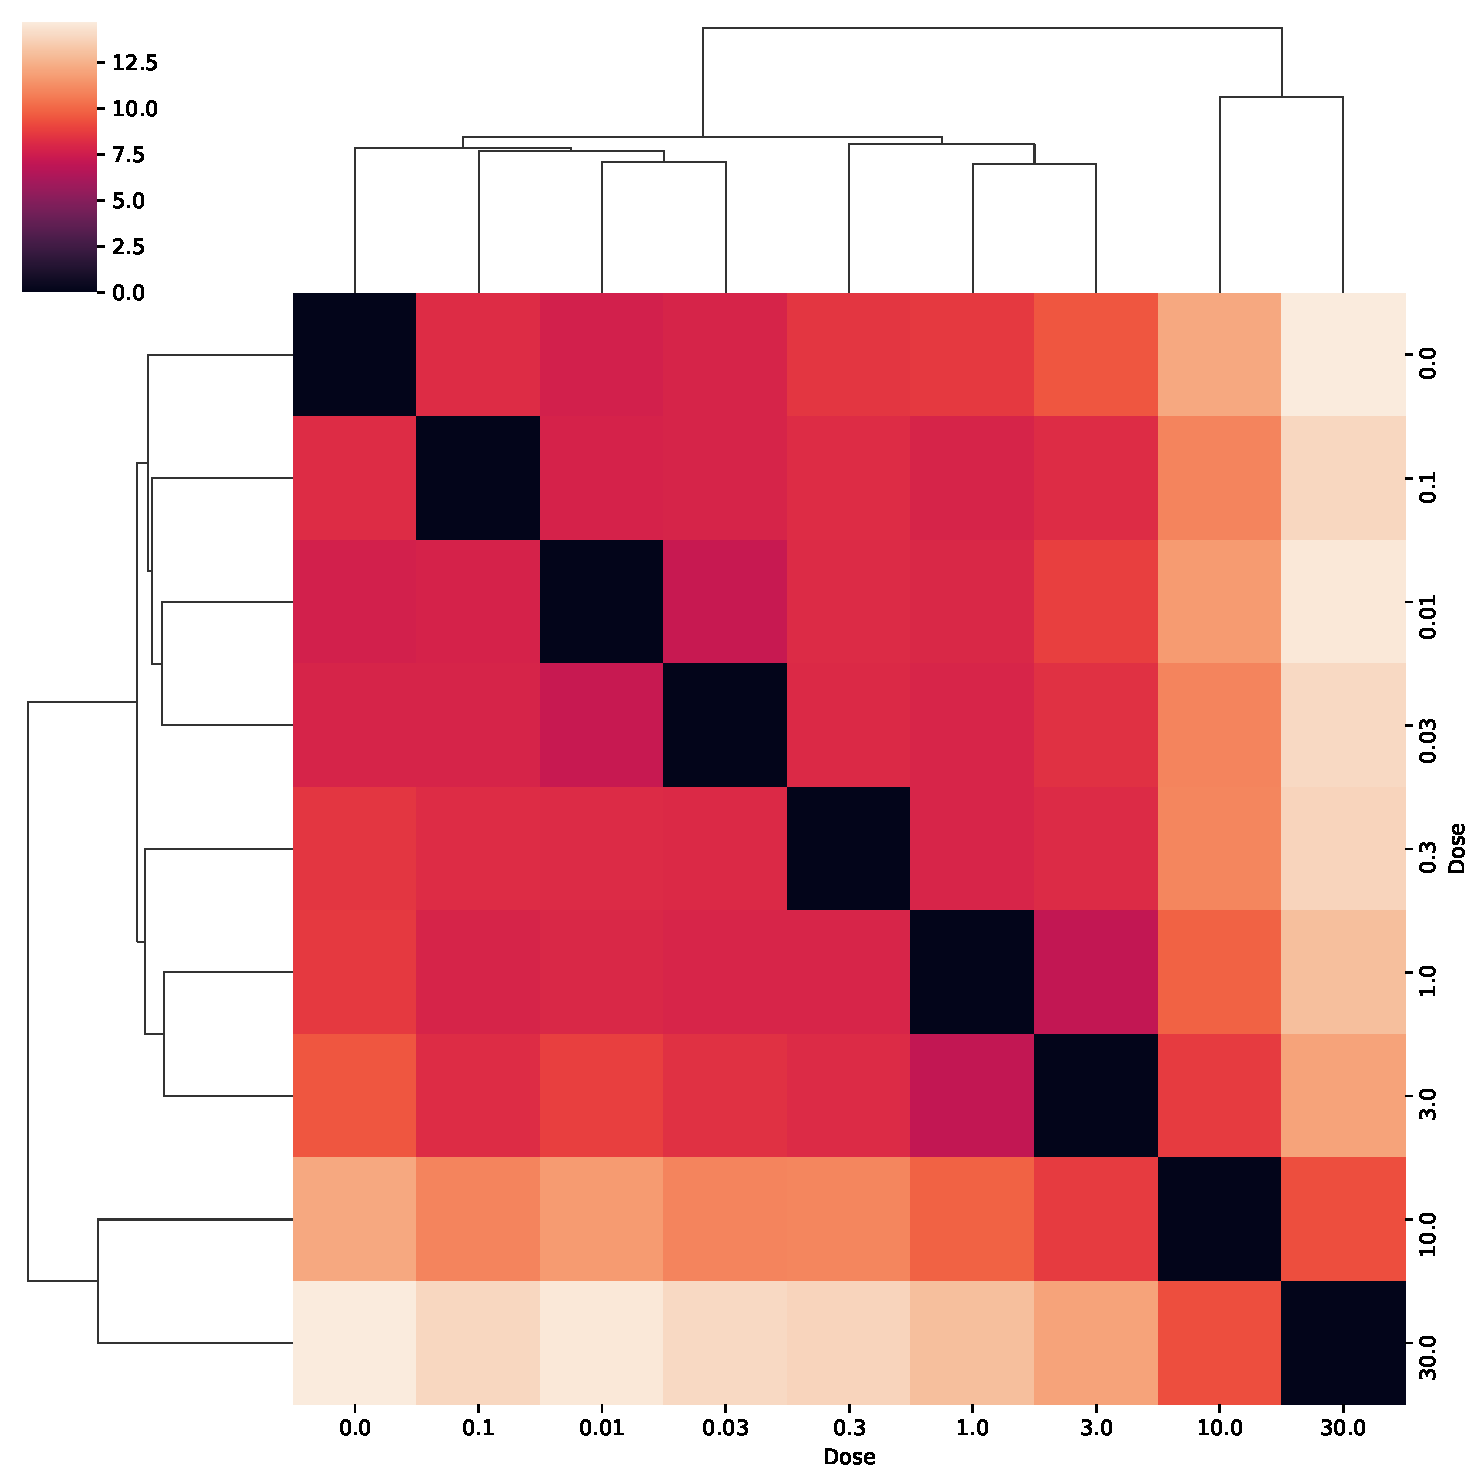
\includegraphics[width=\textwidth]{figures/hepatocytes_central_mean_pairwise_clustermap.pdf}
        \caption{Mean pairwise}
    \end{minipage} \hfill
    \begin{minipage}{0.4\textwidth}
        \centering
        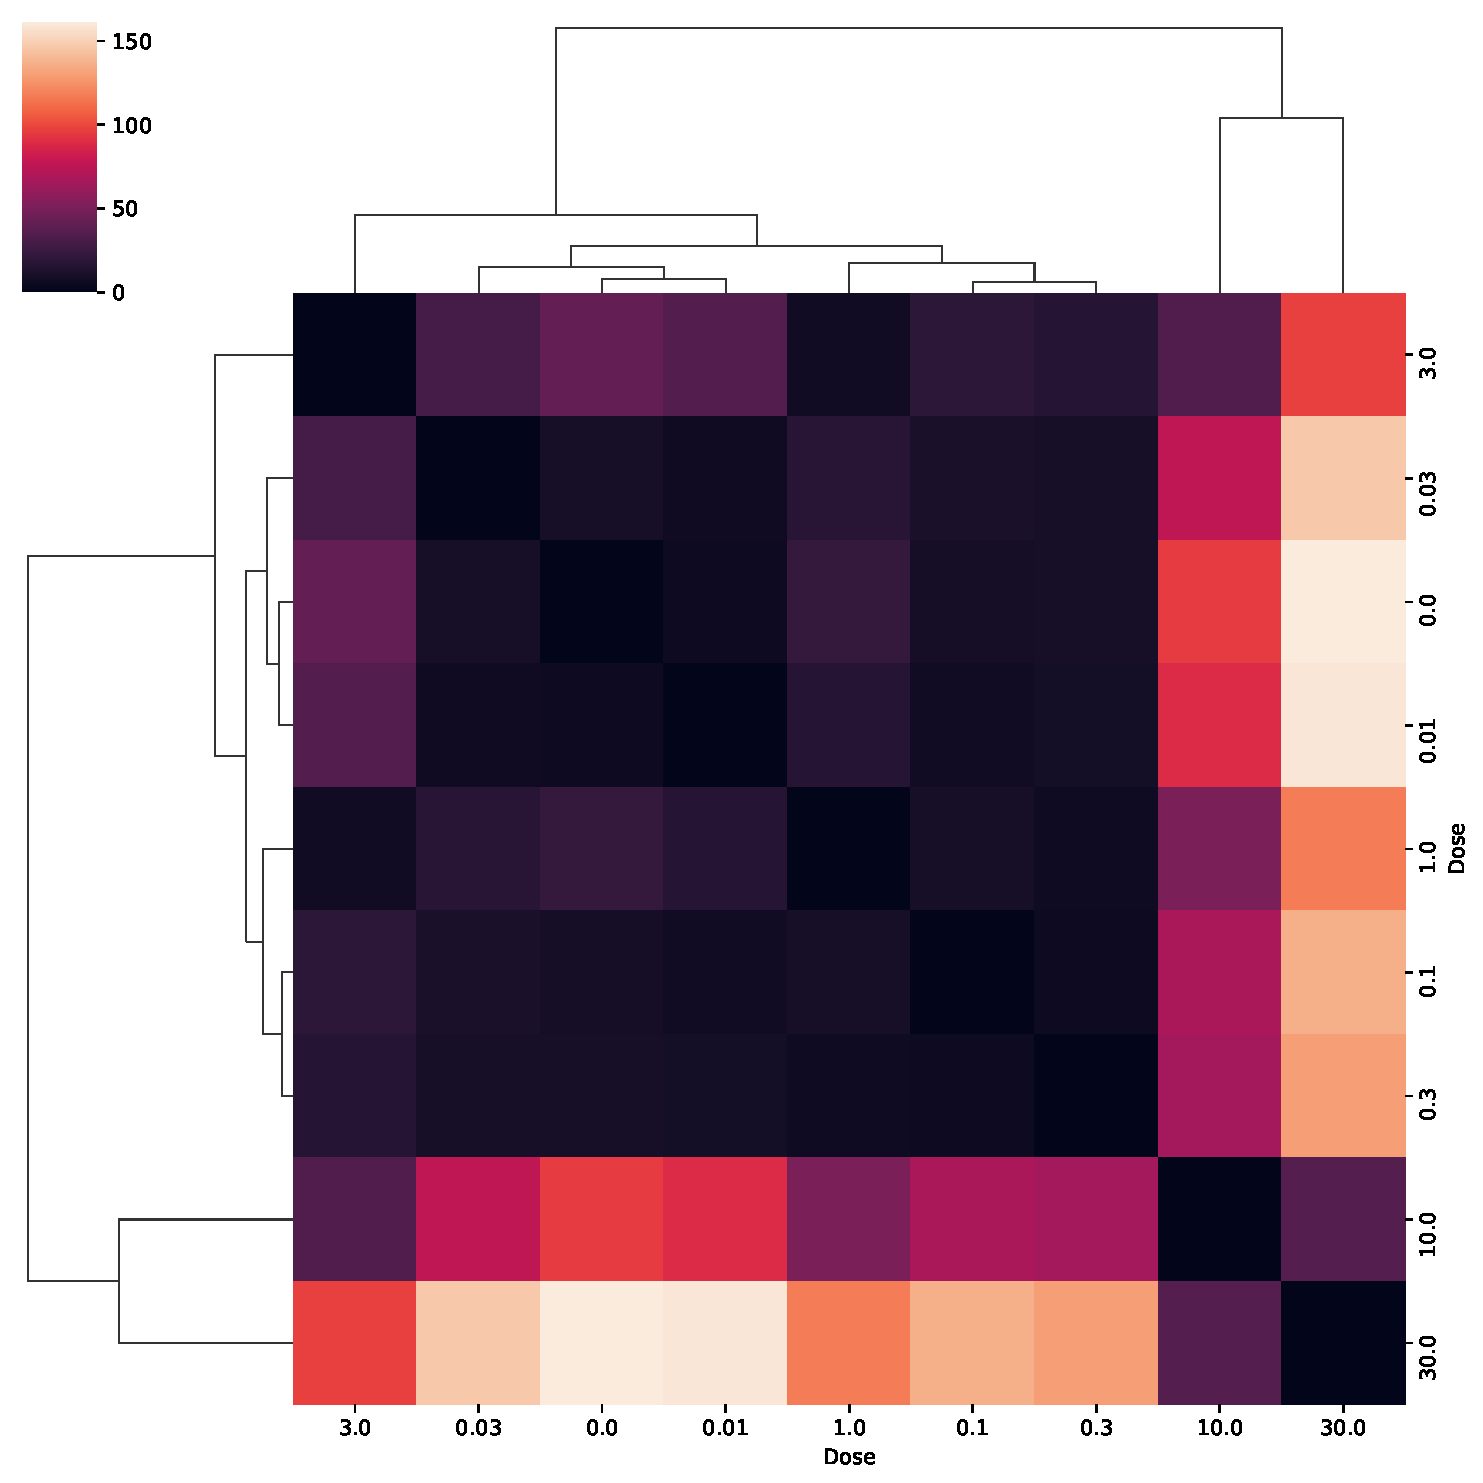
\includegraphics[width=\textwidth]{figures/hepatocytes_central_mmd_clustermap.pdf}
        \caption{MMD}
    \end{minipage}
    \vskip\baselineskip

    \begin{minipage}{0.4\textwidth}
        \centering
        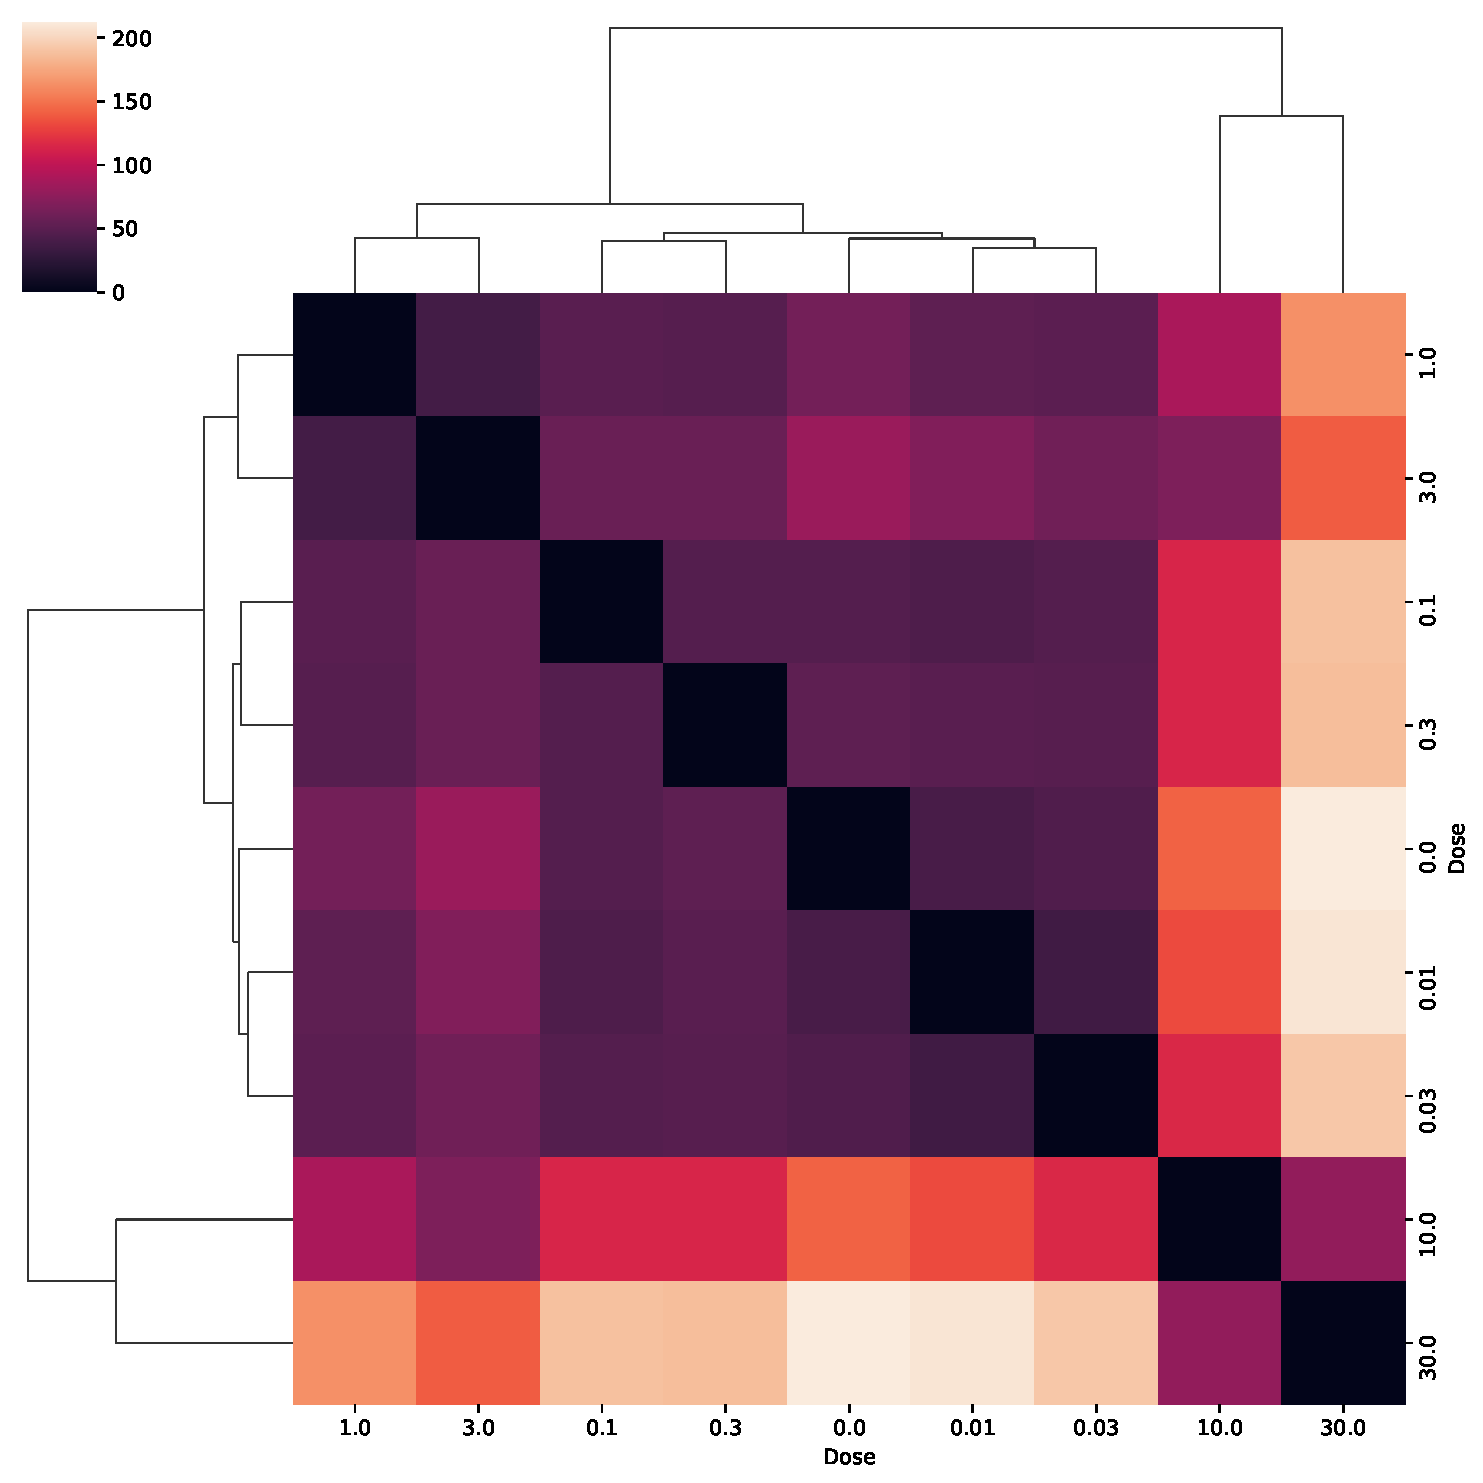
\includegraphics[width=\textwidth]{figures/hepatocytes_central_wasserstein_clustermap.pdf}
        \caption{Wasserstein}
    \end{minipage}
    \caption{Distance metrics for cell type Hepatocytes - central per dosage}
\end{figure}

\begin{figure}
    \centering
    \begin{minipage}{0.4\textwidth}
        \centering
        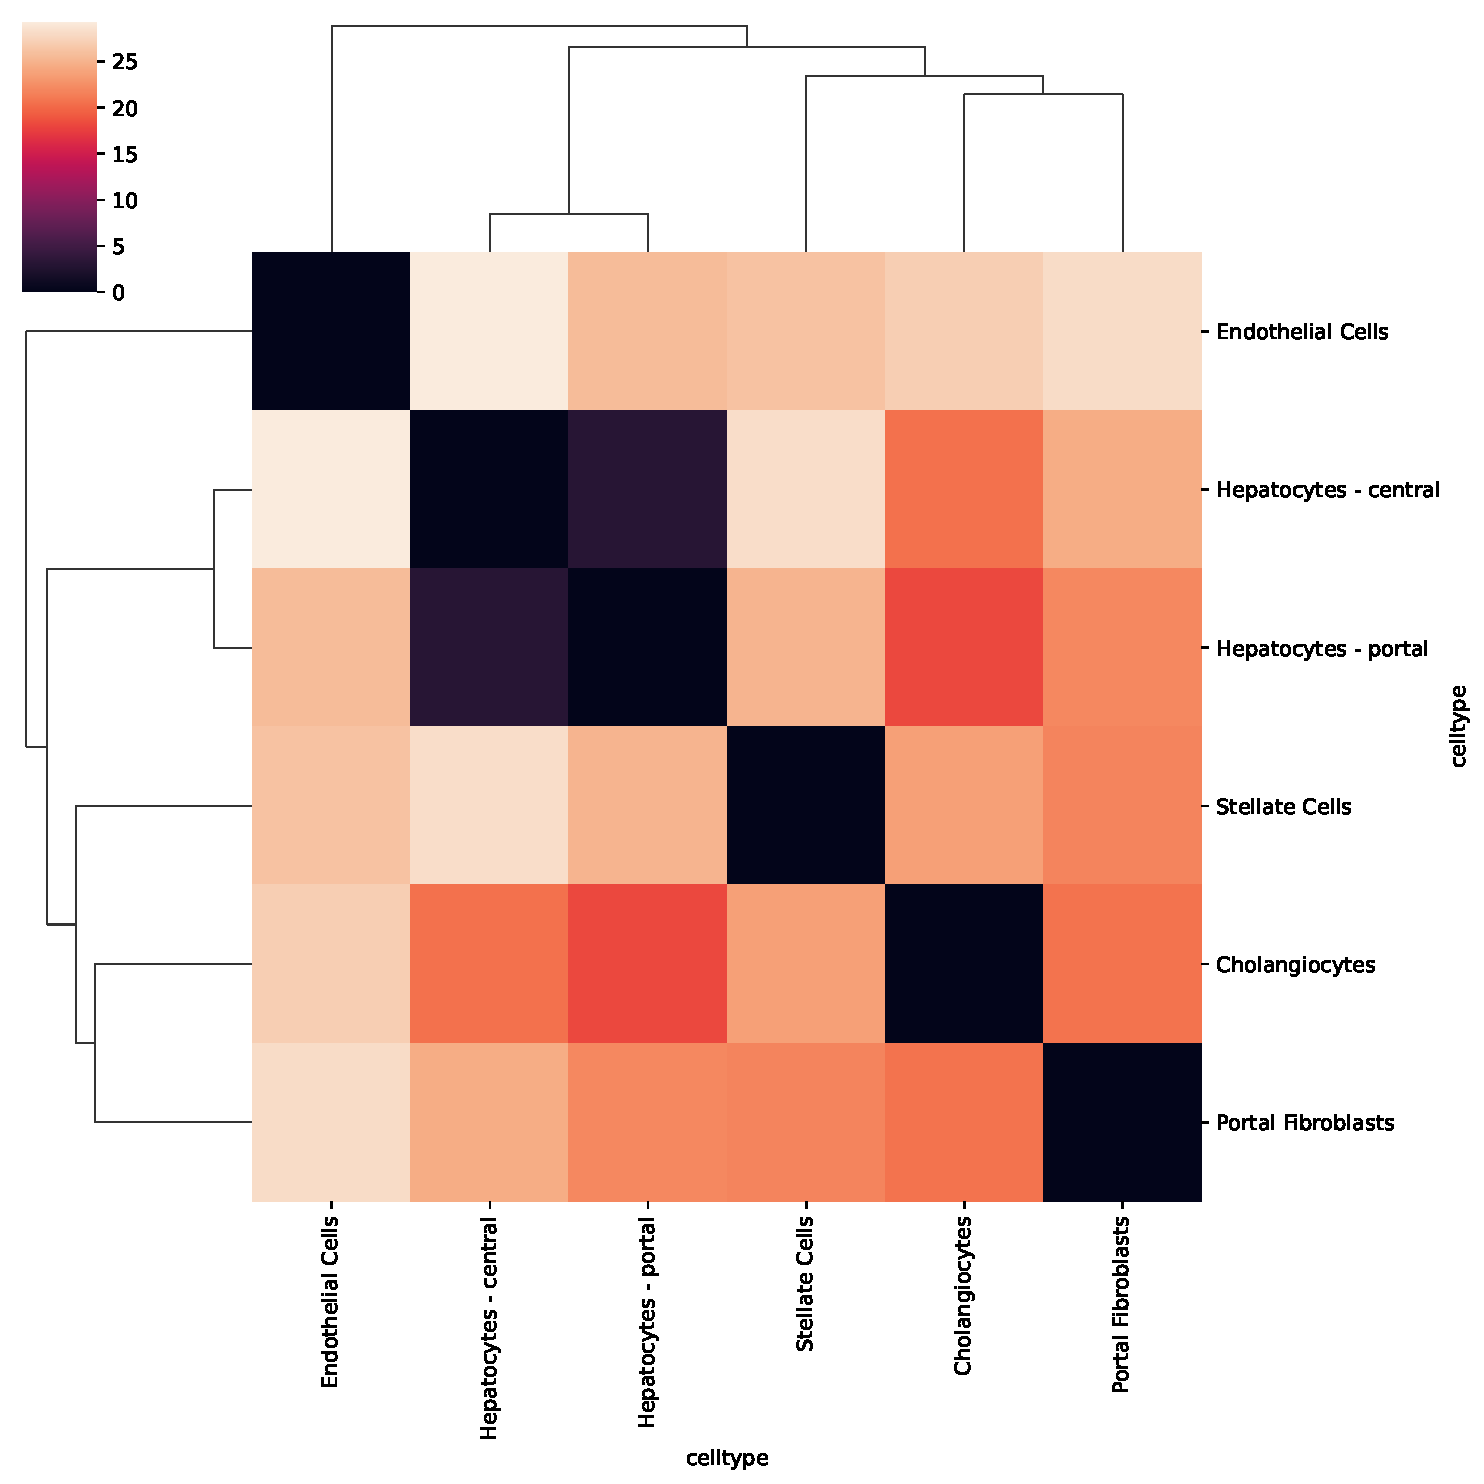
\includegraphics[width=\textwidth]{figures/dose_highest_edistance_clustermap.pdf}
        \caption{E-distance}
    \end{minipage} \hfill
    \begin{minipage}{0.4\textwidth}
        \centering
        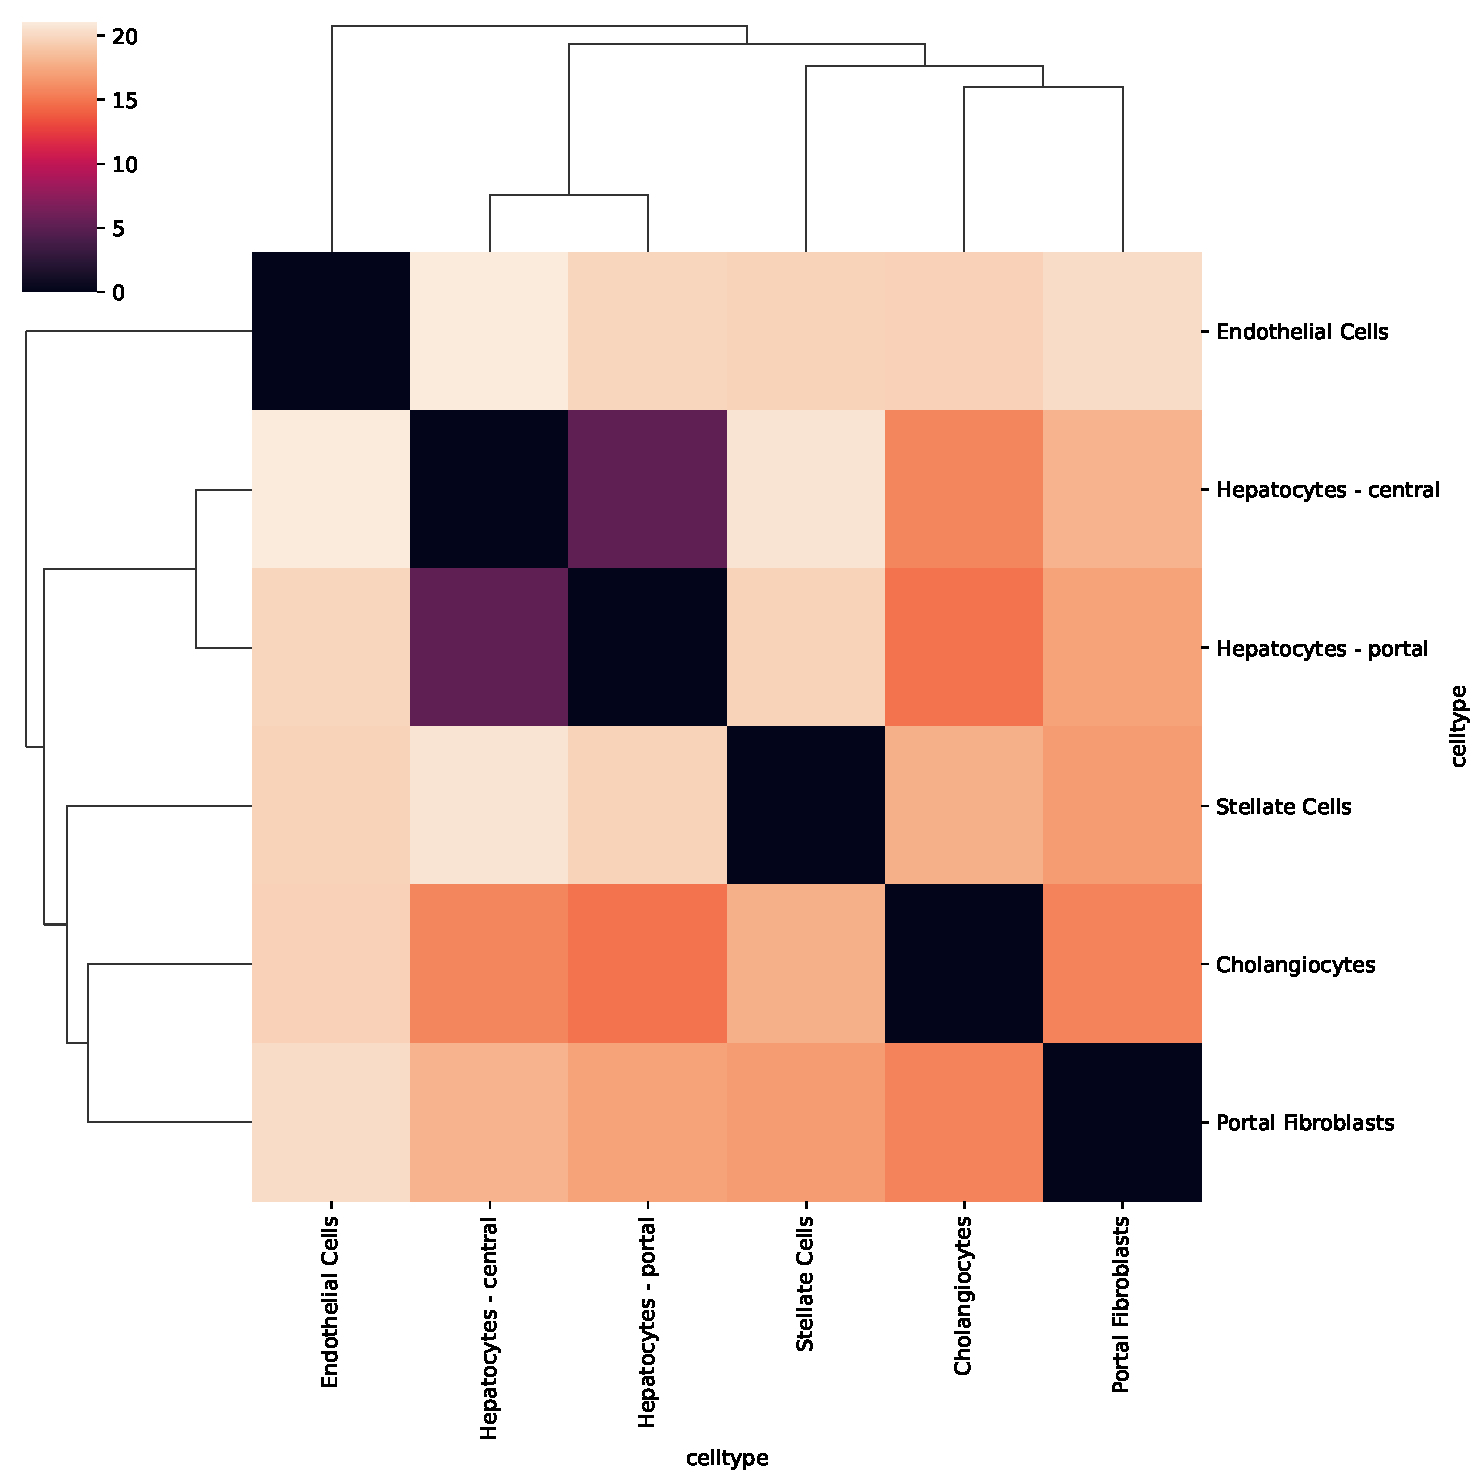
\includegraphics[width=\textwidth]{figures/dose_highest_euclidean_clustermap.pdf}
        \caption{Euclidean}
    \end{minipage}
    \vskip\baselineskip

    \begin{minipage}{0.4\textwidth}
        \centering
        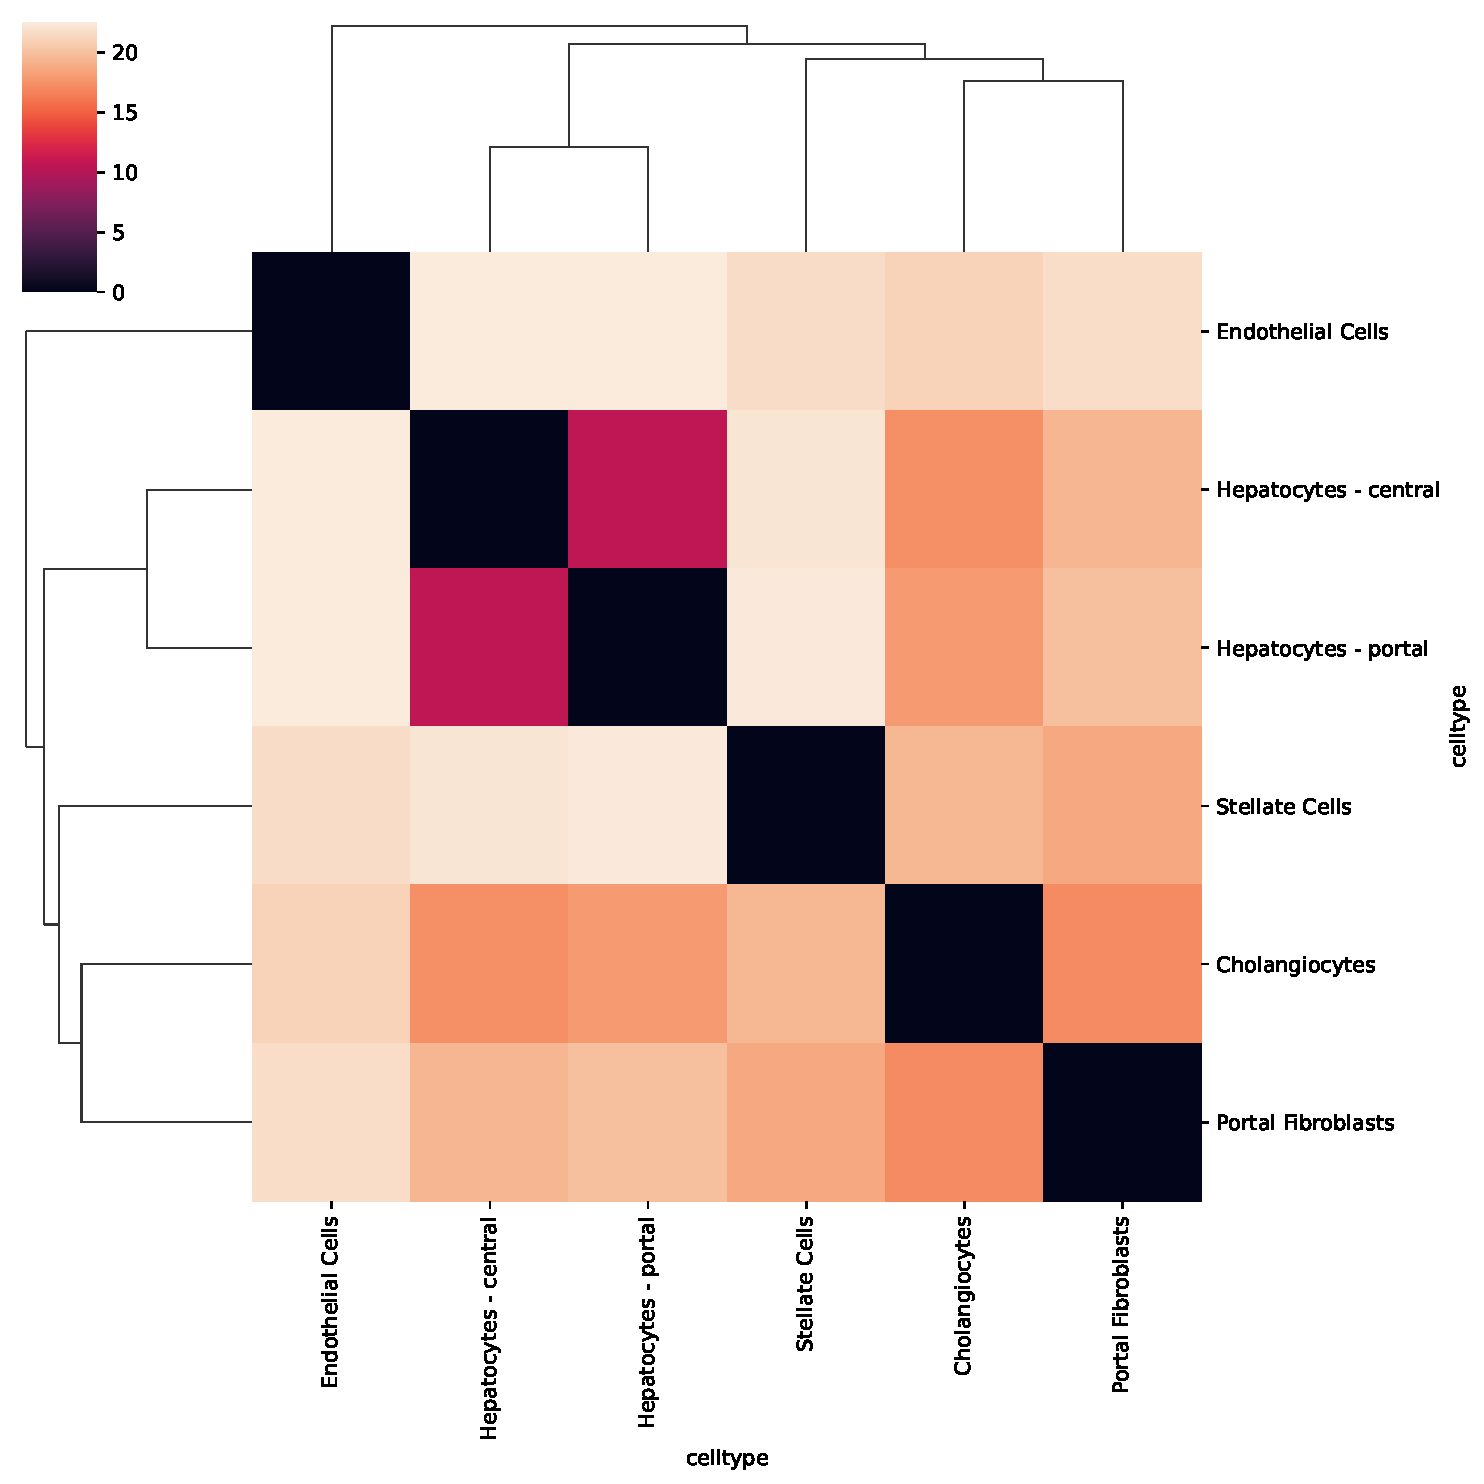
\includegraphics[width=\textwidth]{figures/dose_highest_mean_pairwise_clustermap.pdf}
        \caption{Mean pairwise}
    \end{minipage} \hfill
    \begin{minipage}{0.4\textwidth}
        \centering
        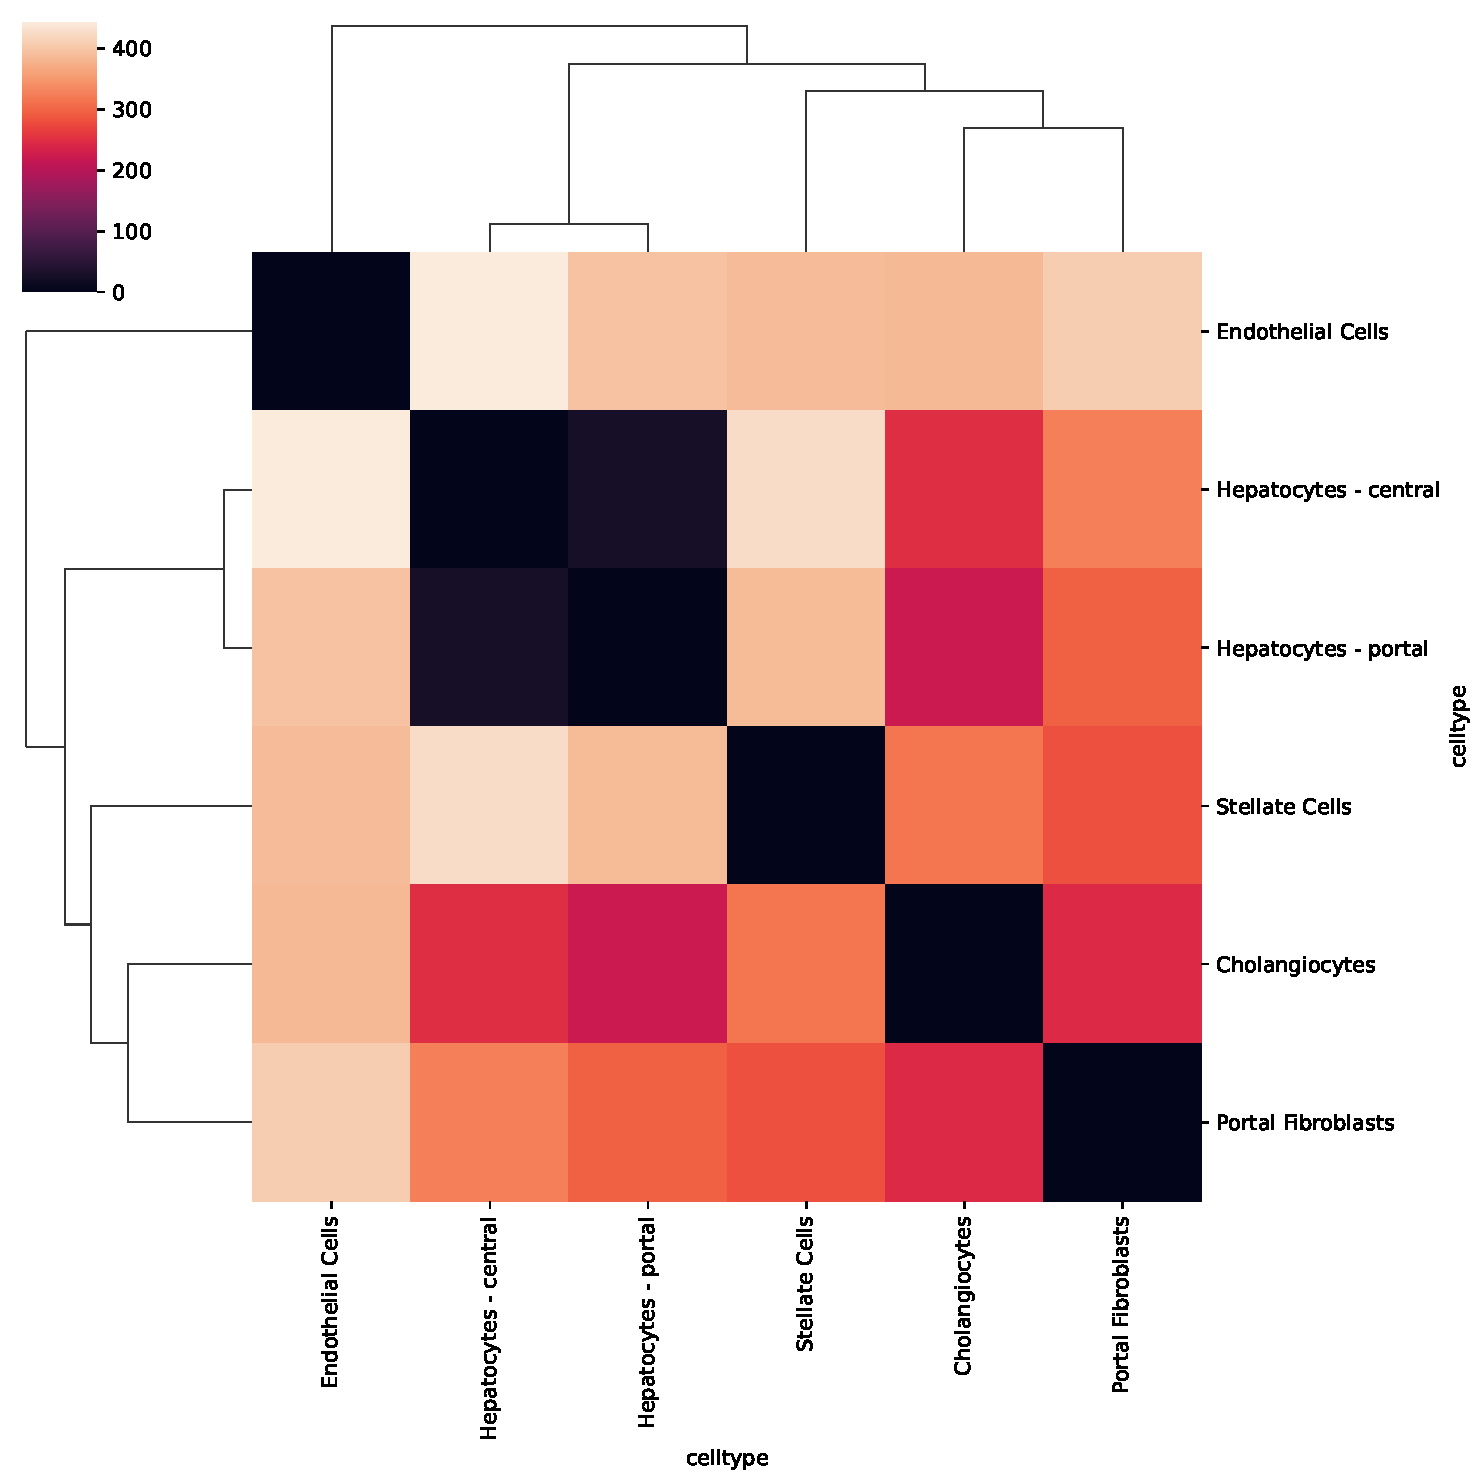
\includegraphics[width=\textwidth]{figures/dose_highest_mmd_clustermap.pdf}
        \caption{MMD}
    \end{minipage}
    \vskip\baselineskip

    \begin{minipage}{0.4\textwidth}
        \centering
        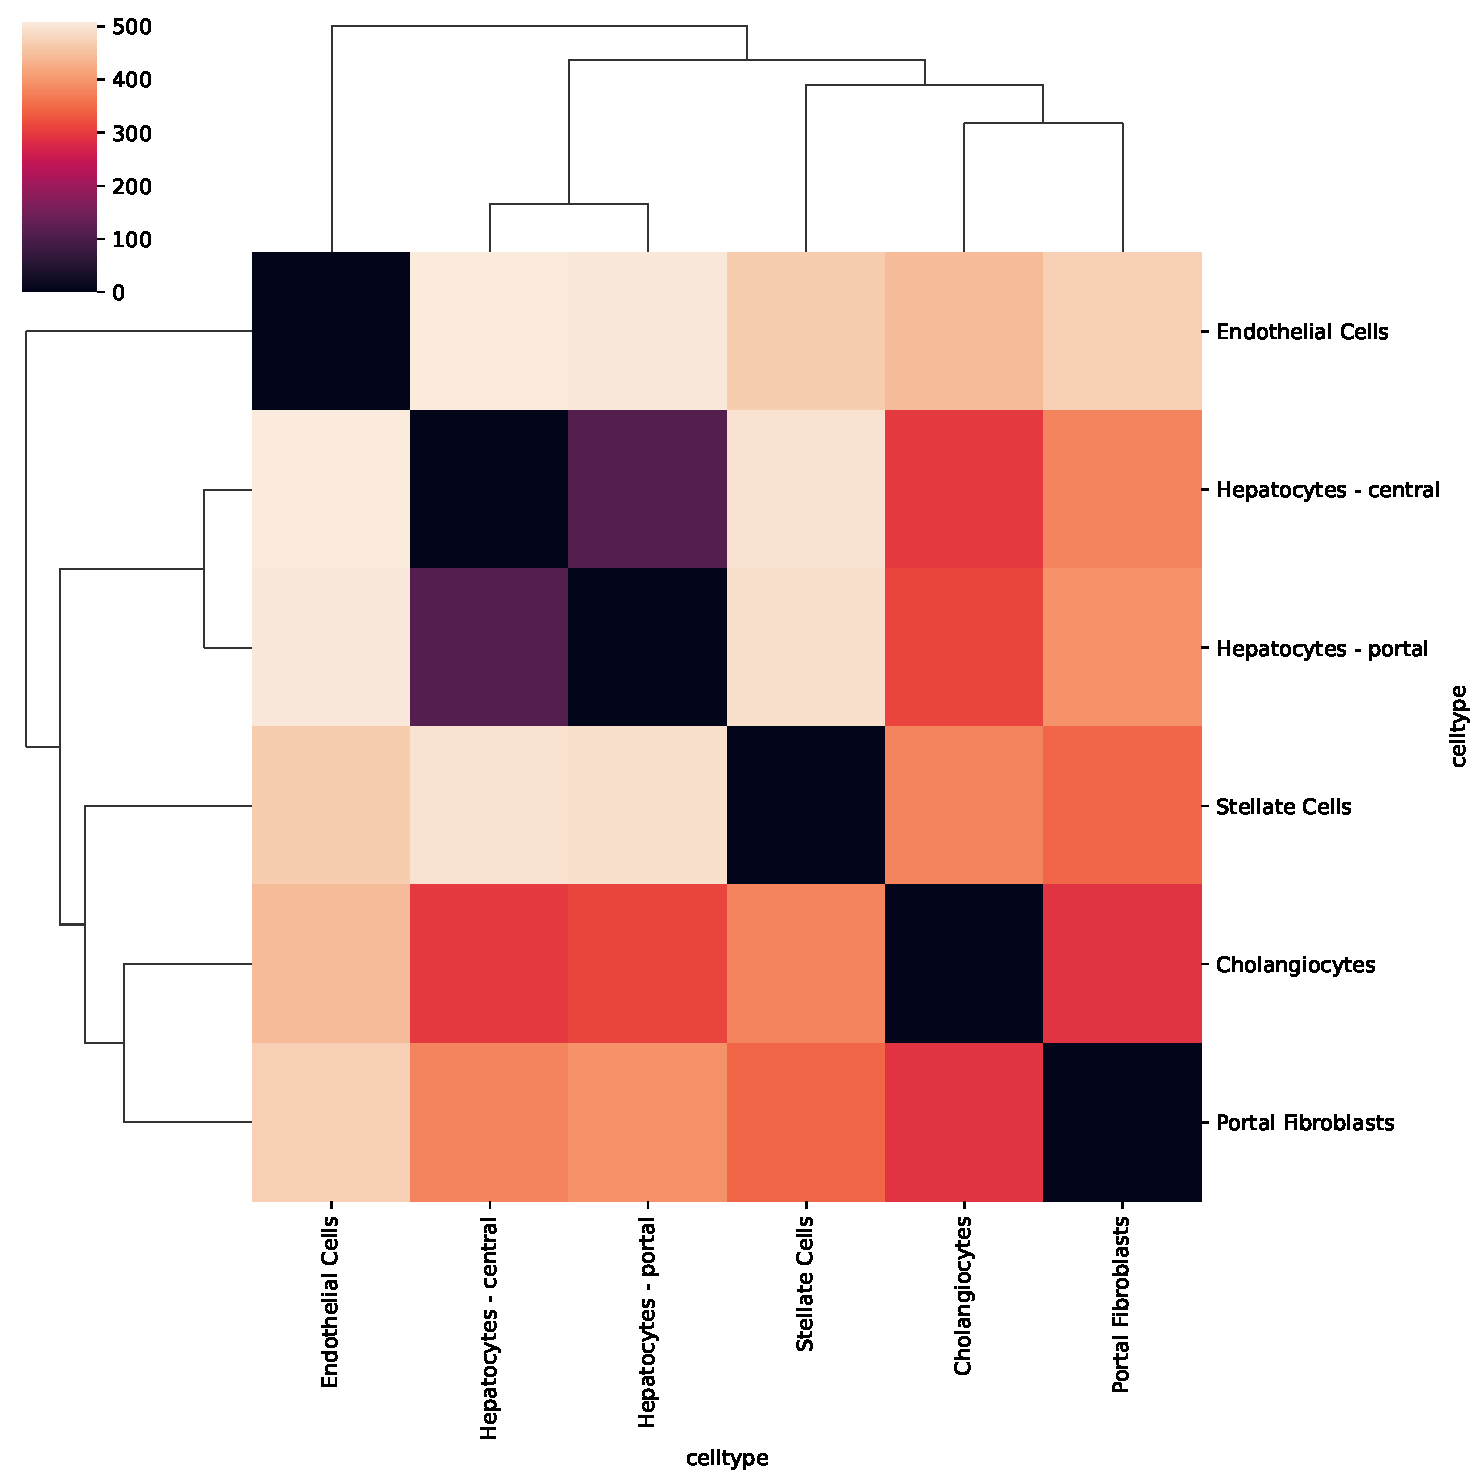
\includegraphics[width=\textwidth]{figures/dose_highest_wasserstein_clustermap.pdf}
        \caption{Wasserstein}
    \end{minipage}
    \caption{Distance metrics for dosage highest 30 $\mu g/kg$ per cell type}
\end{figure}

\begin{figure}
    \centering
    \begin{minipage}{0.4\textwidth}
        \centering
        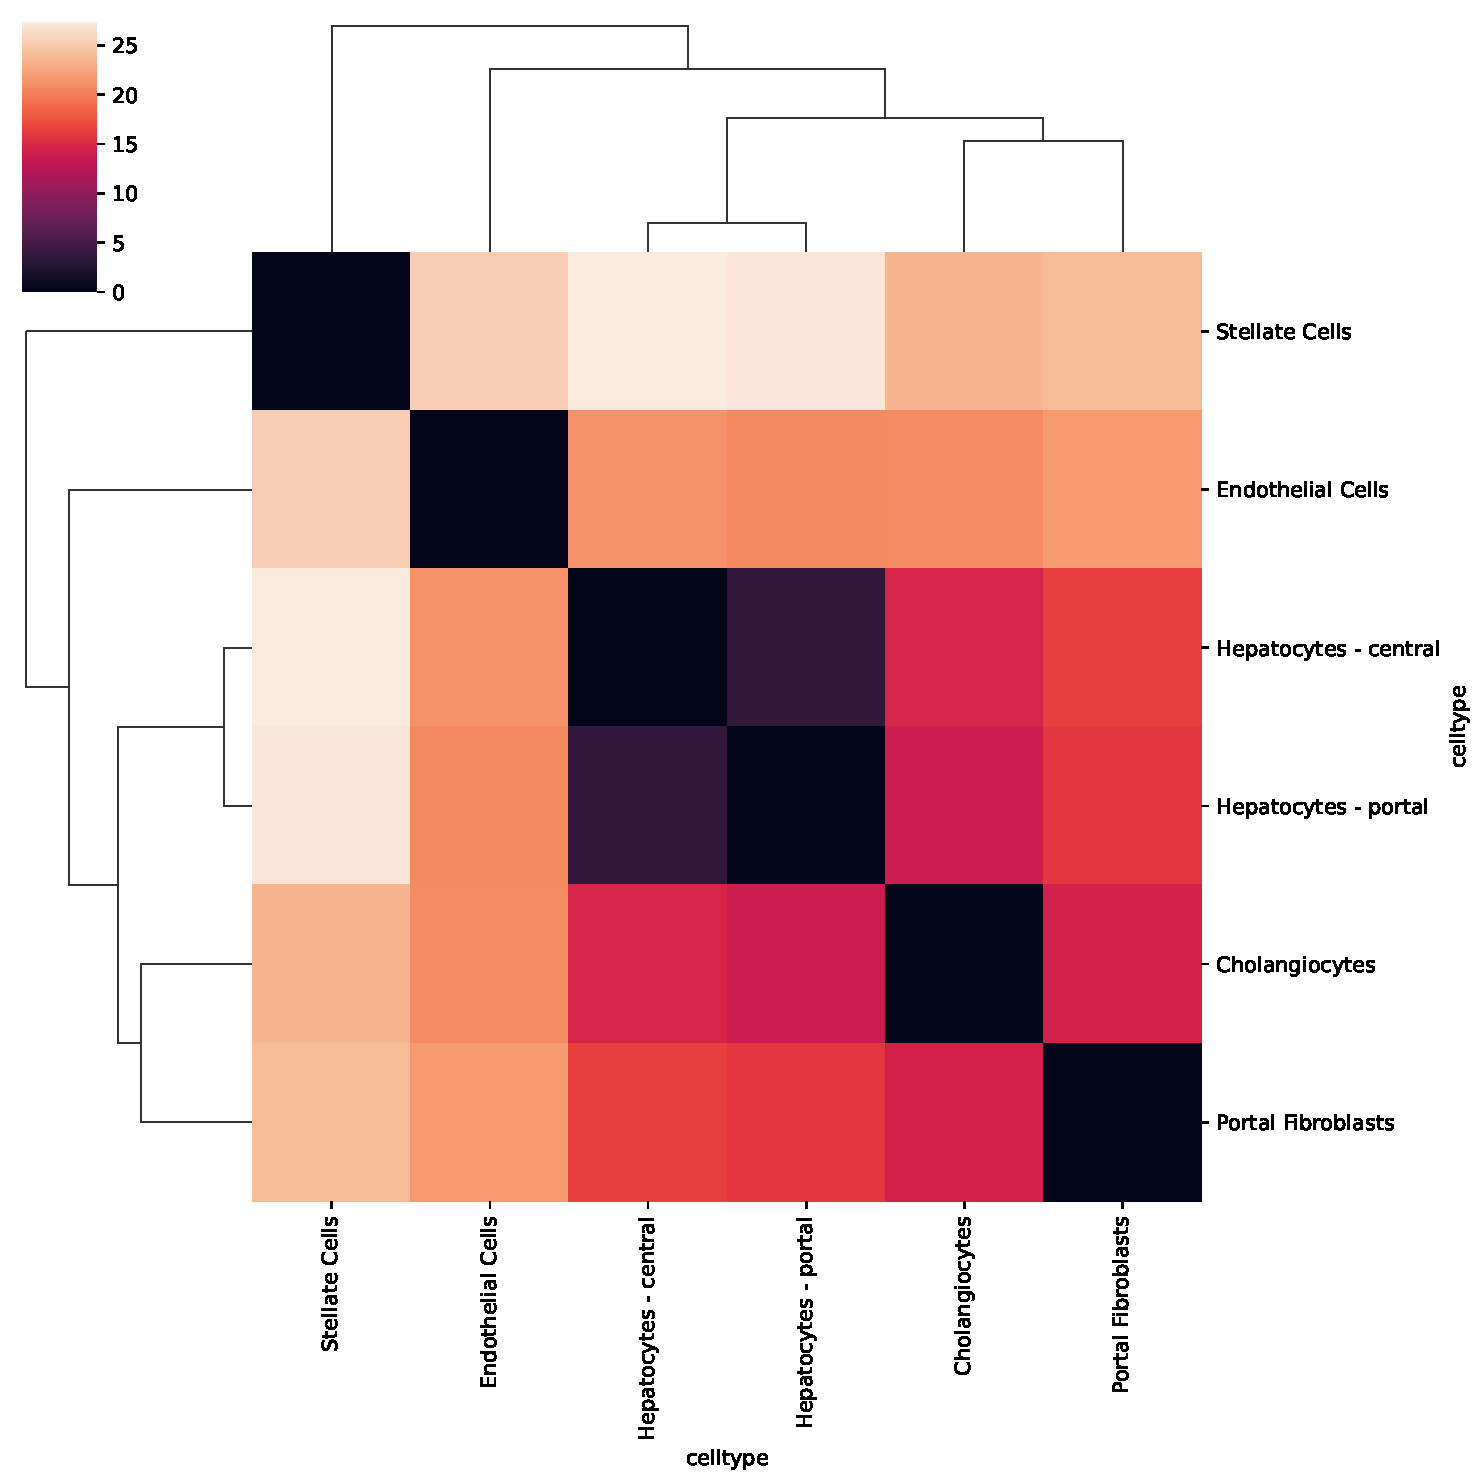
\includegraphics[width=\textwidth]{figures/dose_lowest_edistance_clustermap.pdf}
        \caption{E-distance}
    \end{minipage} \hfill
    \begin{minipage}{0.4\textwidth}
        \centering
        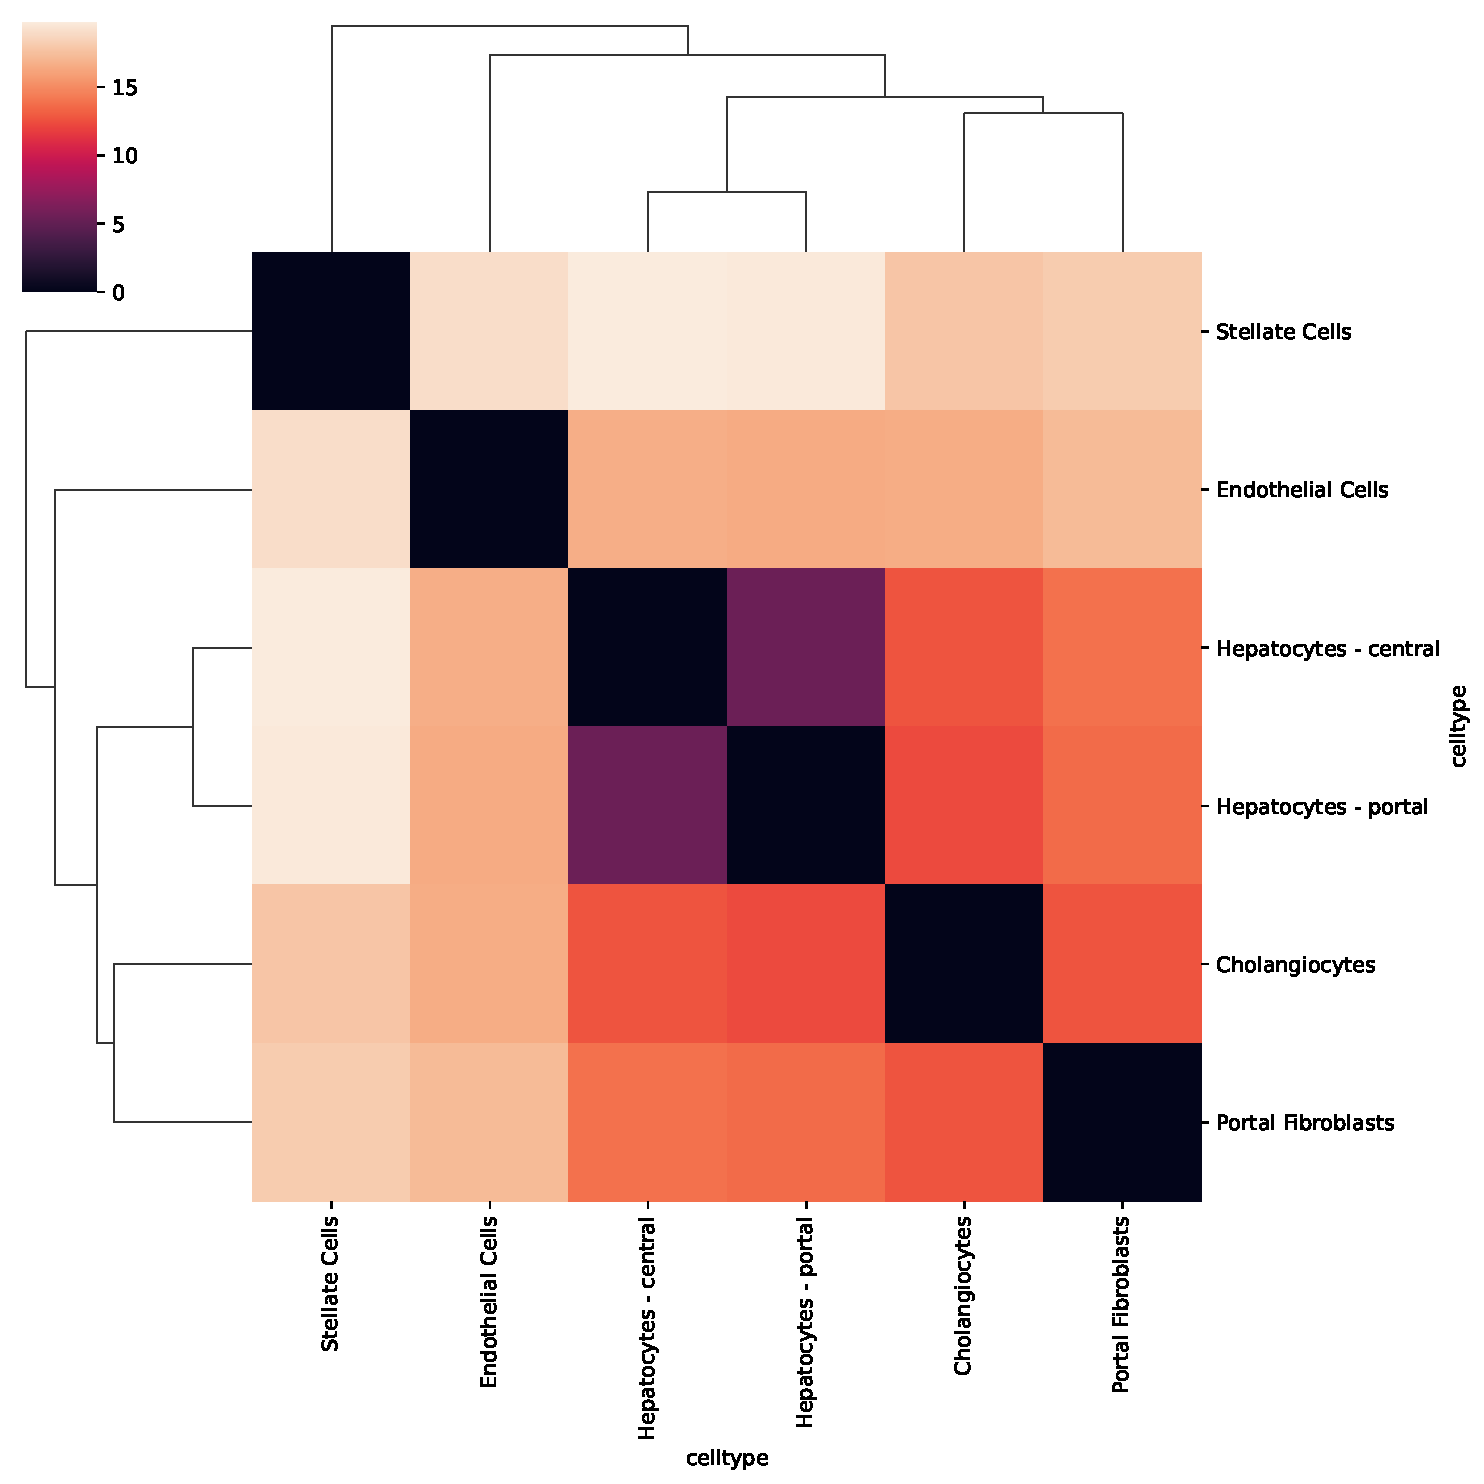
\includegraphics[width=\textwidth]{figures/dose_lowest_euclidean_clustermap.pdf}
        \caption{Euclidean}
    \end{minipage}
    \vskip\baselineskip

    \begin{minipage}{0.4\textwidth}
        \centering
        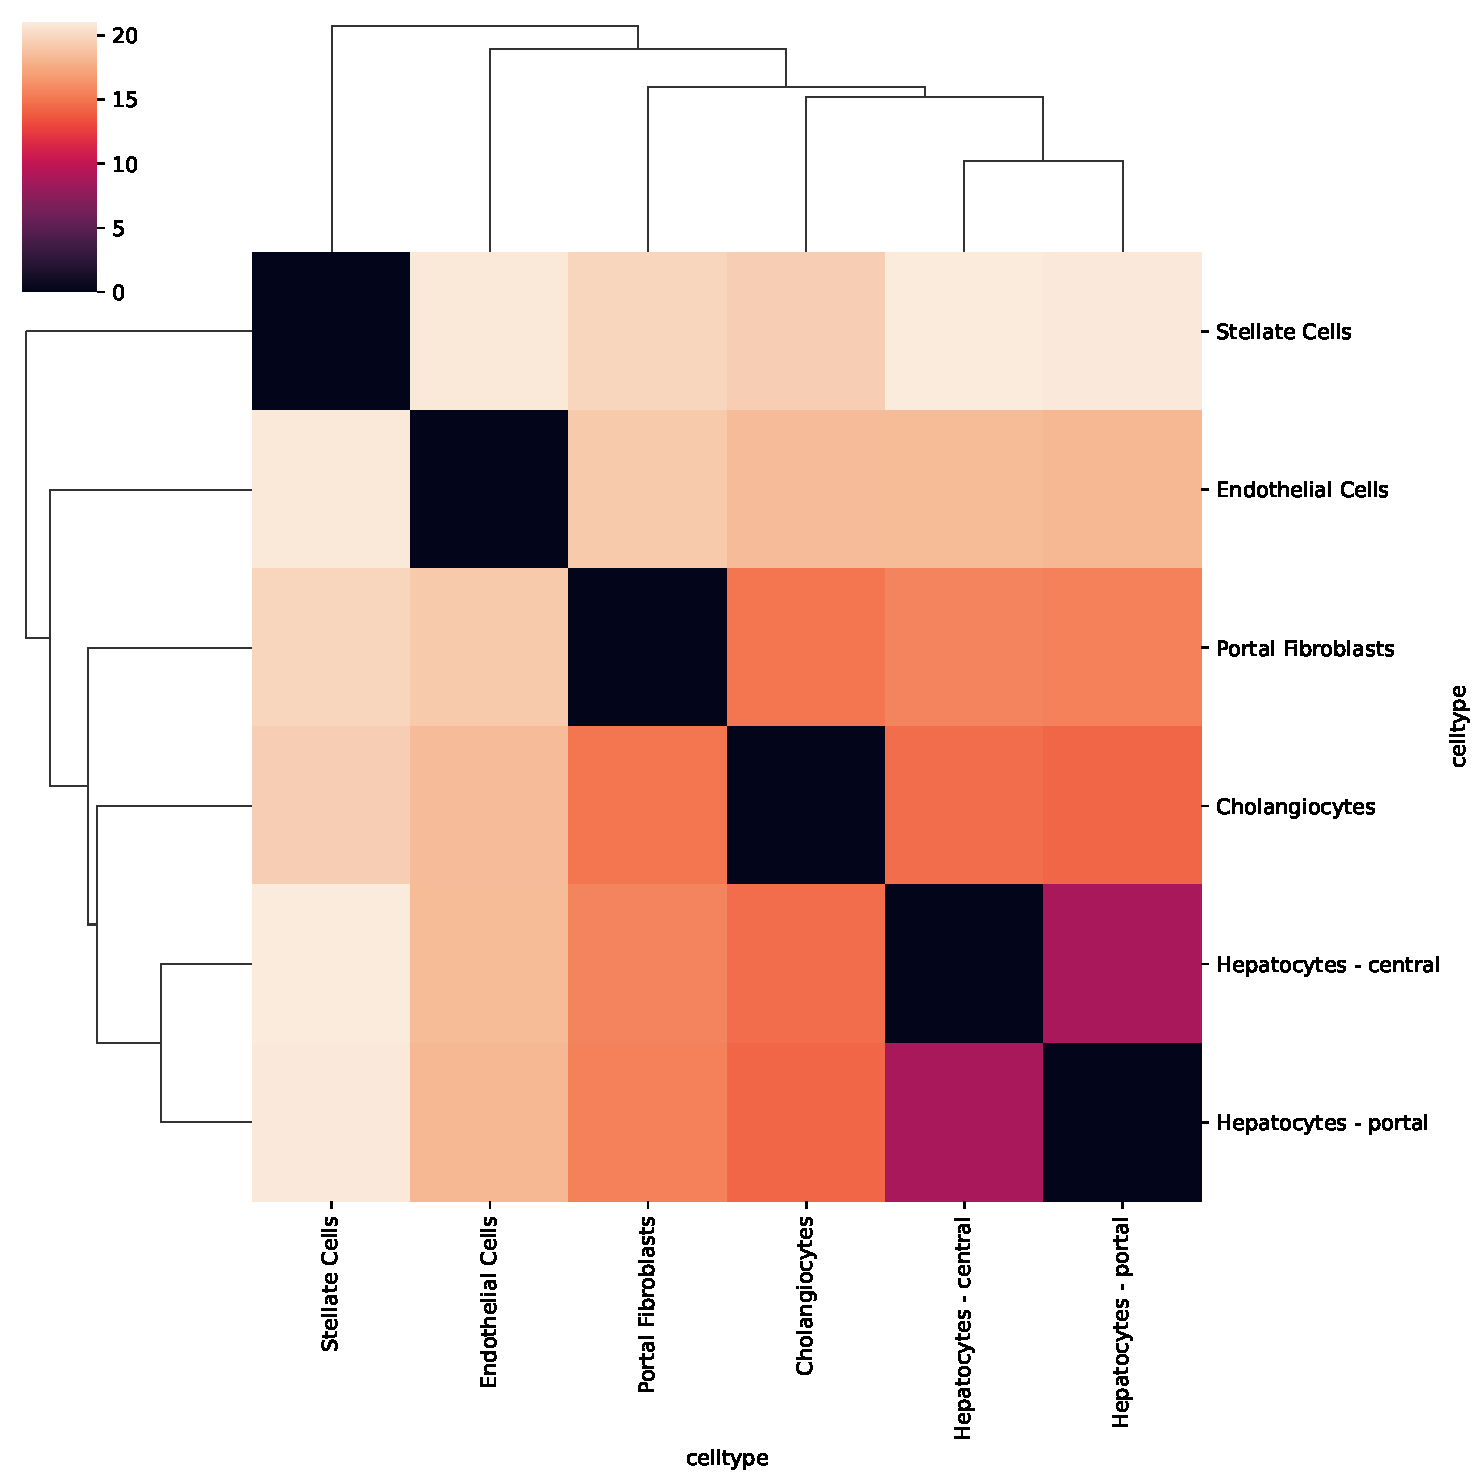
\includegraphics[width=\textwidth]{figures/dose_lowest_mean_pairwise_clustermap.pdf}
        \caption{Mean pairwise}
    \end{minipage} \hfill
    \begin{minipage}{0.4\textwidth}
        \centering
        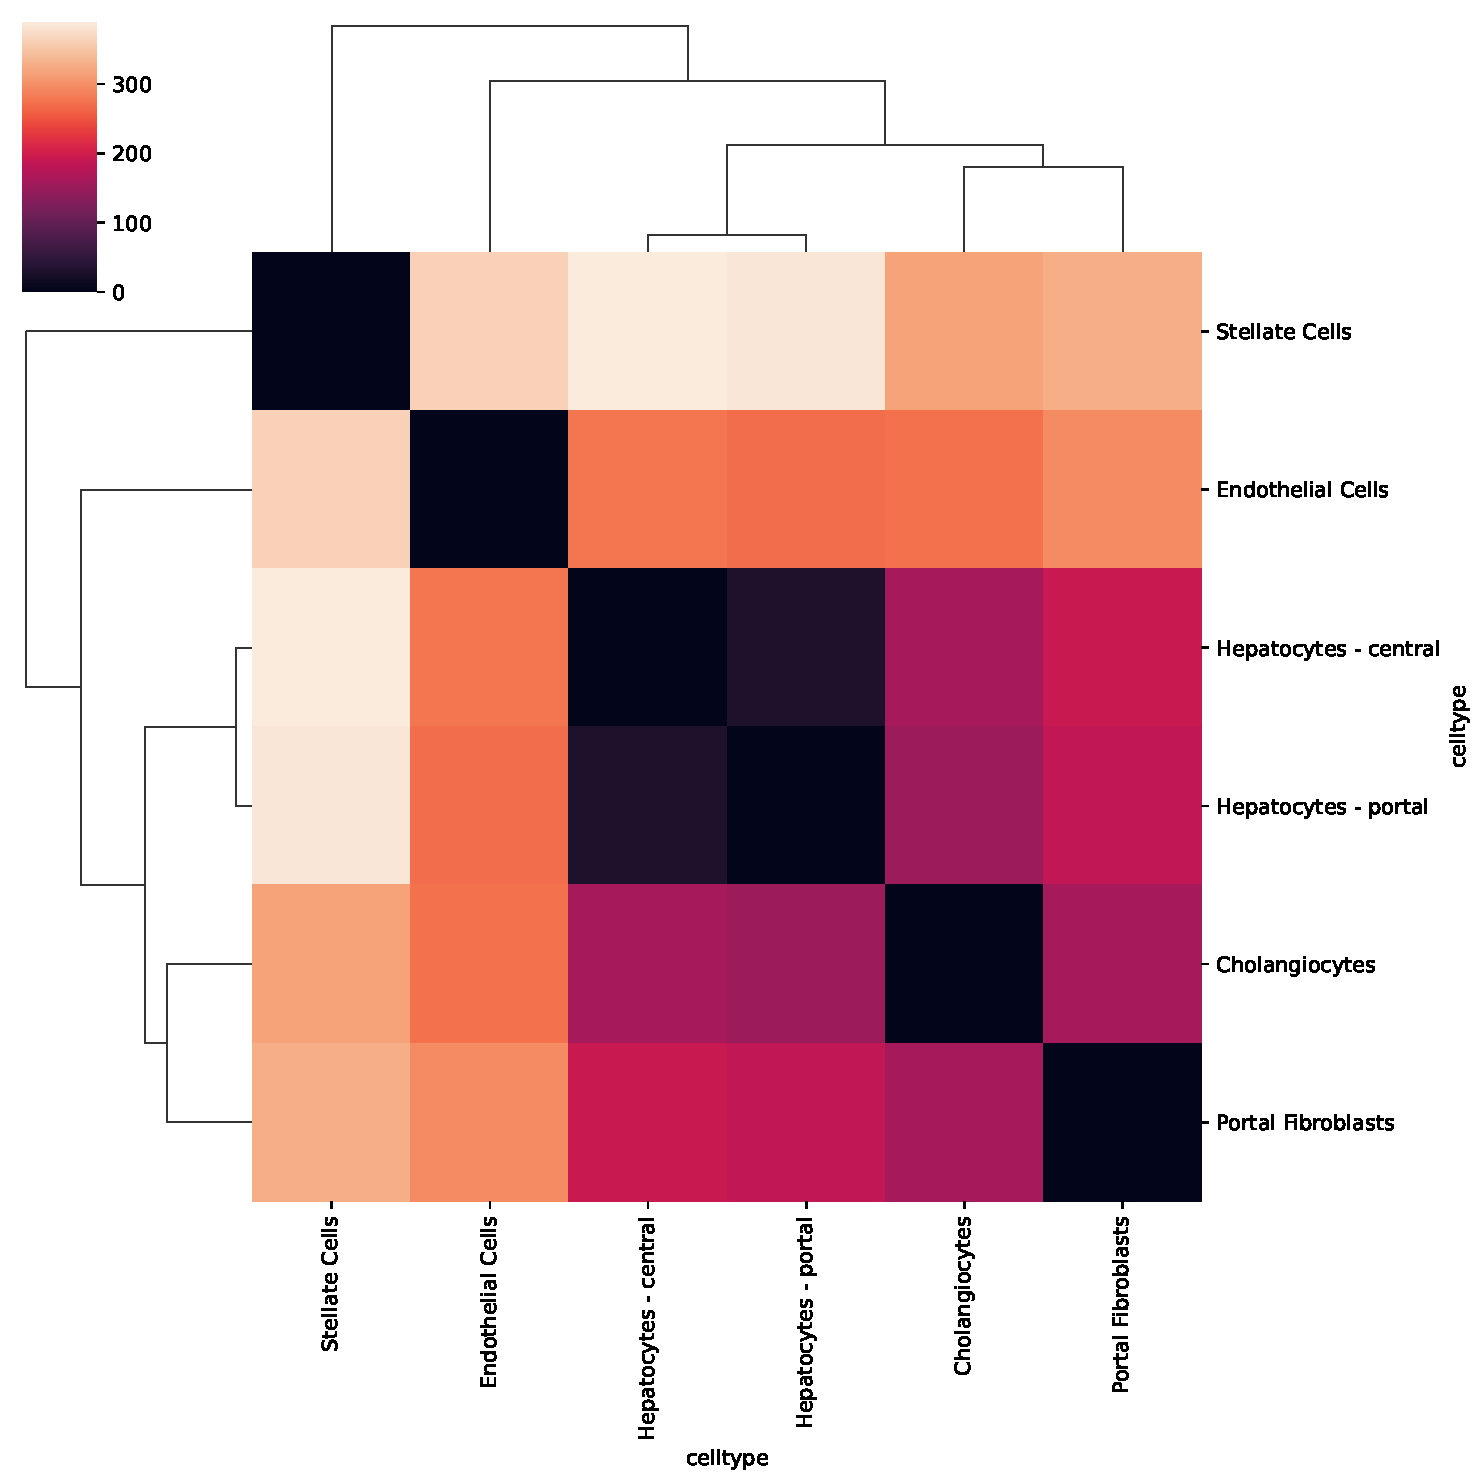
\includegraphics[width=\textwidth]{figures/dose_lowest_mmd_clustermap.pdf}
        \caption{MMD}
    \end{minipage}
    \vskip\baselineskip

    \begin{minipage}{0.4\textwidth}
        \centering
        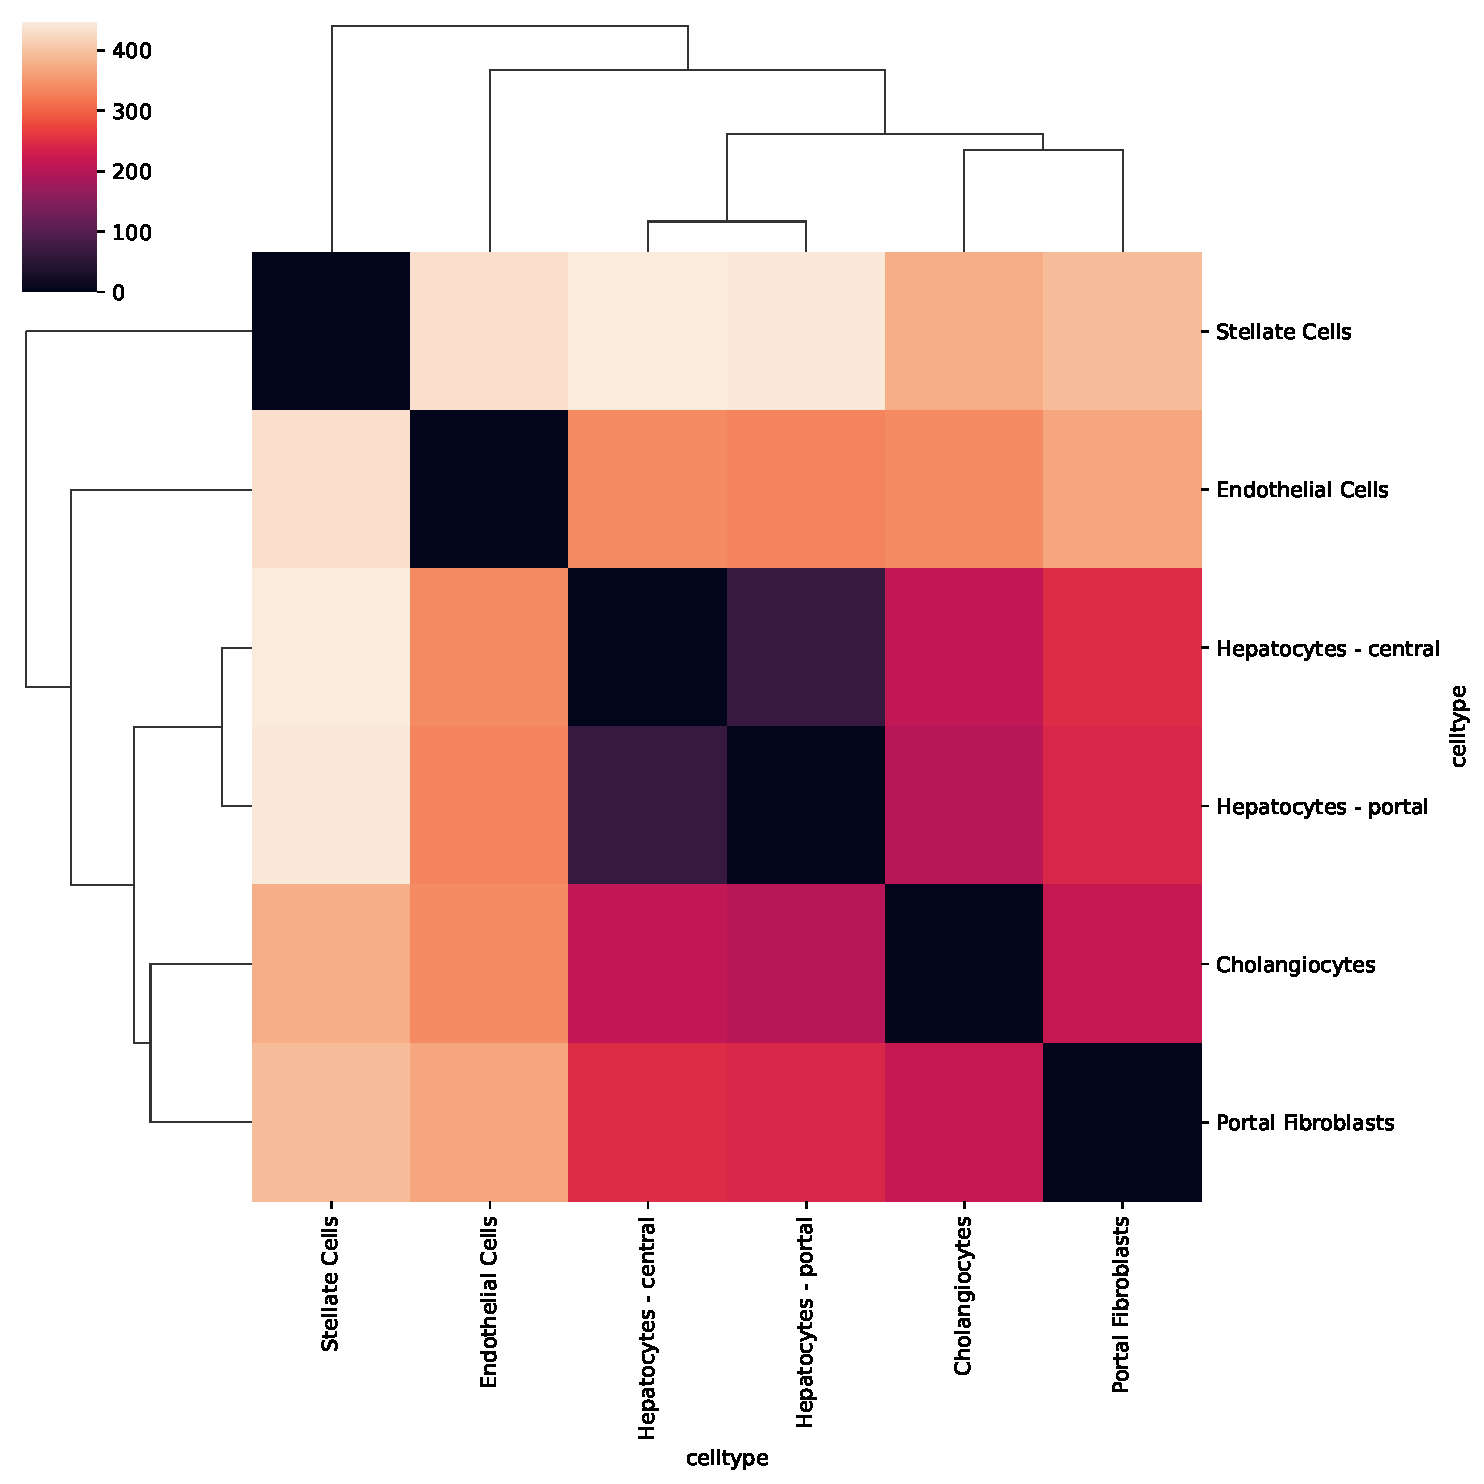
\includegraphics[width=\textwidth]{figures/dose_lowest_wasserstein_clustermap.pdf}
        \caption{Wasserstein}
    \end{minipage}
    \caption{Distance metrics for lowest dosage 0.01 $\mu g/kg$ per cell type}
\end{figure}

\clearpage


\subsection{PBMC dataset}


\begin{figure}[h]
    \centering
    \begin{subfigure}[t]{0.49\textwidth}
        \centering
        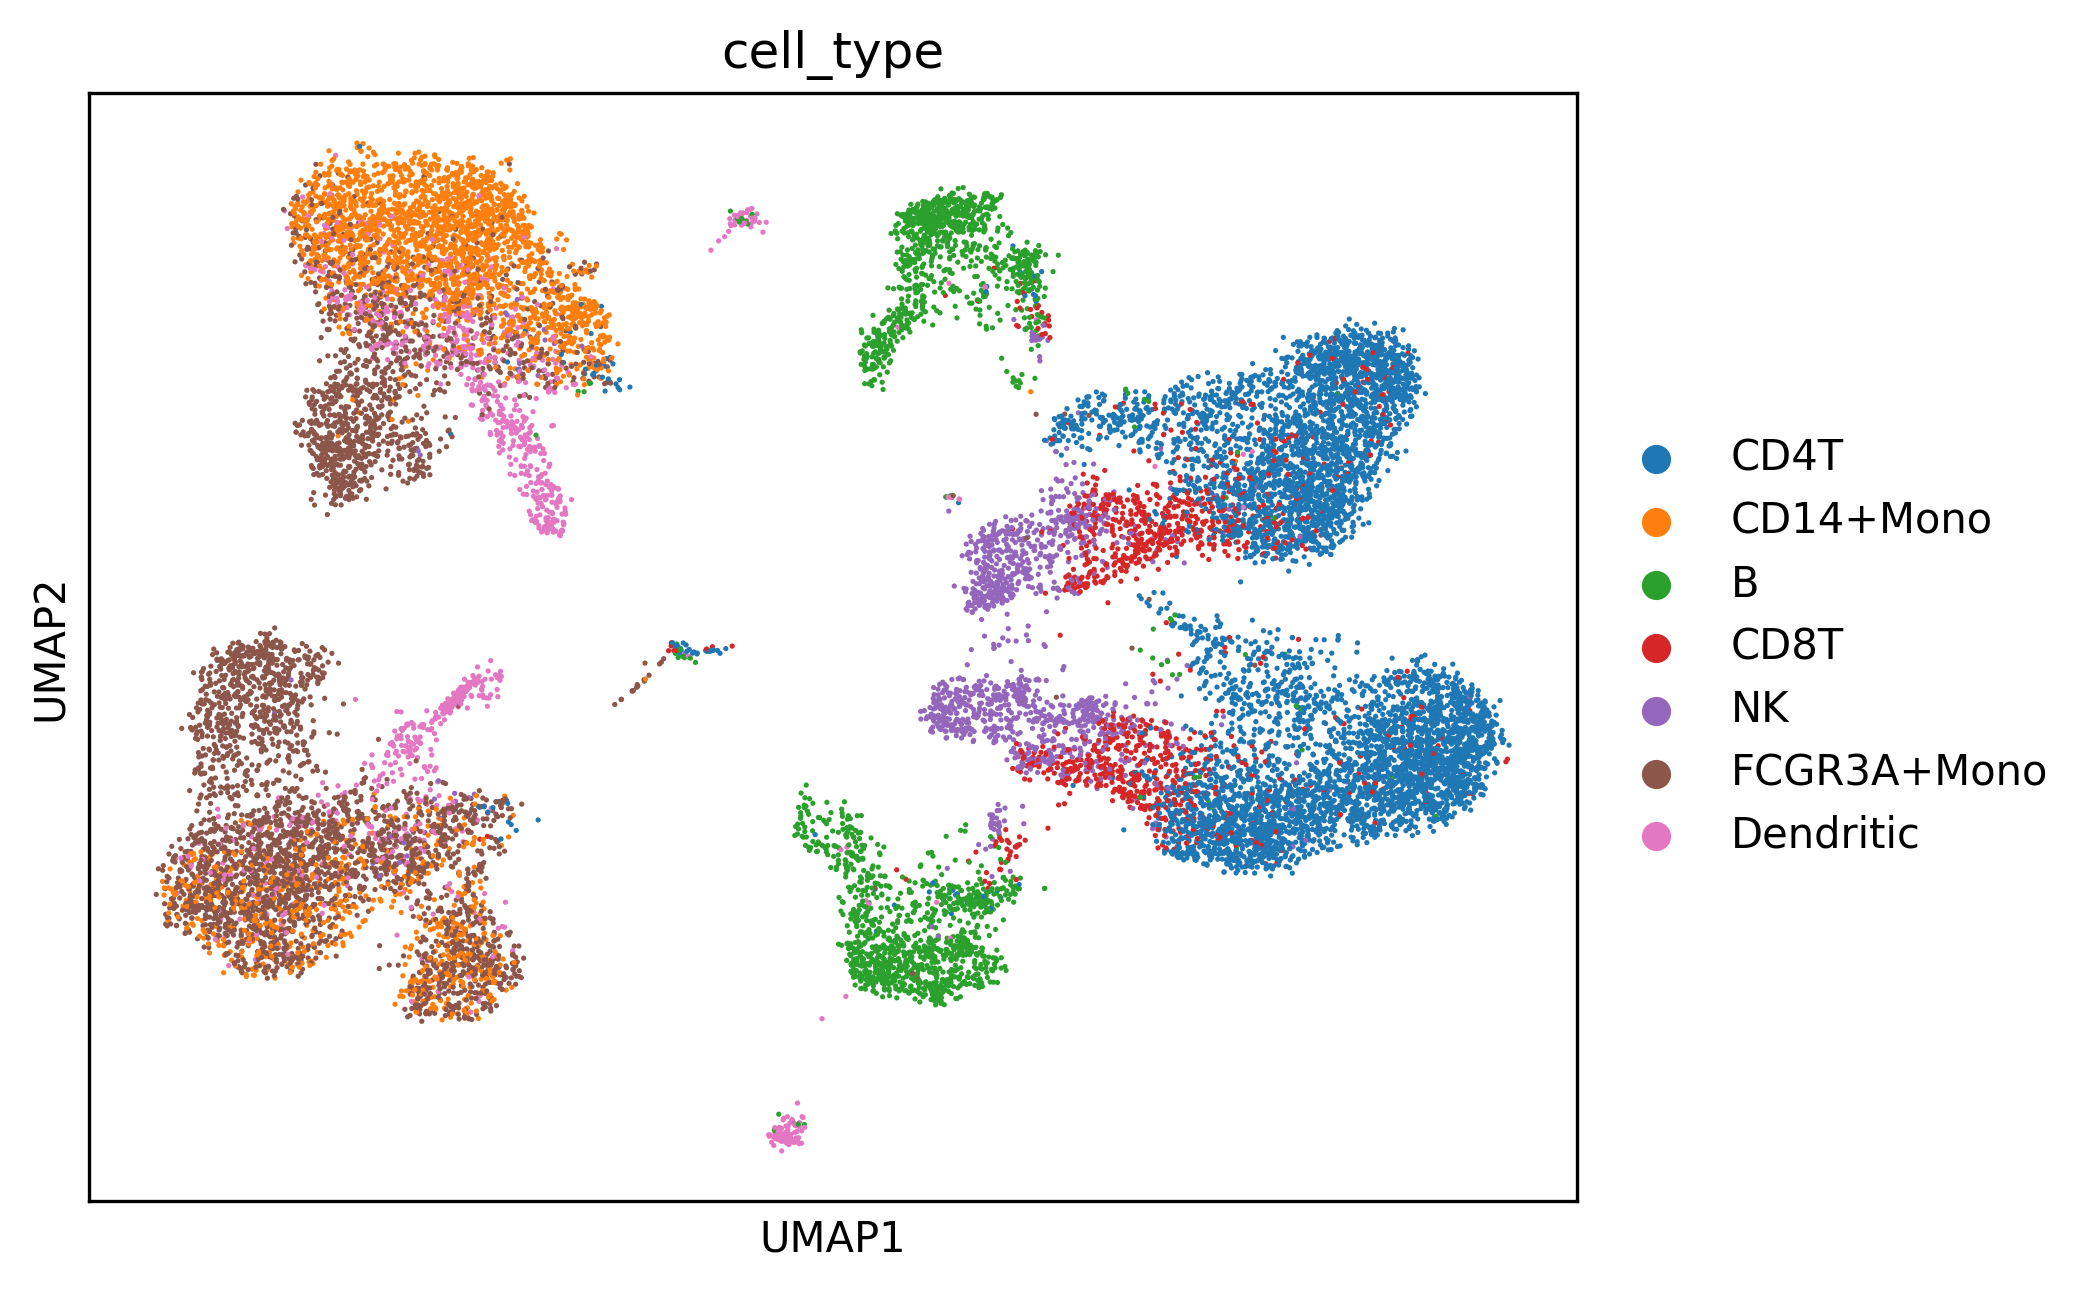
\includegraphics[width=\textwidth]{figures/pbmc_cell_umap.png}
        \caption{}
        \label{fig:figure1}
    \end{subfigure}
    \hfill
    \begin{subfigure}[t]{0.49\textwidth}
        \centering
        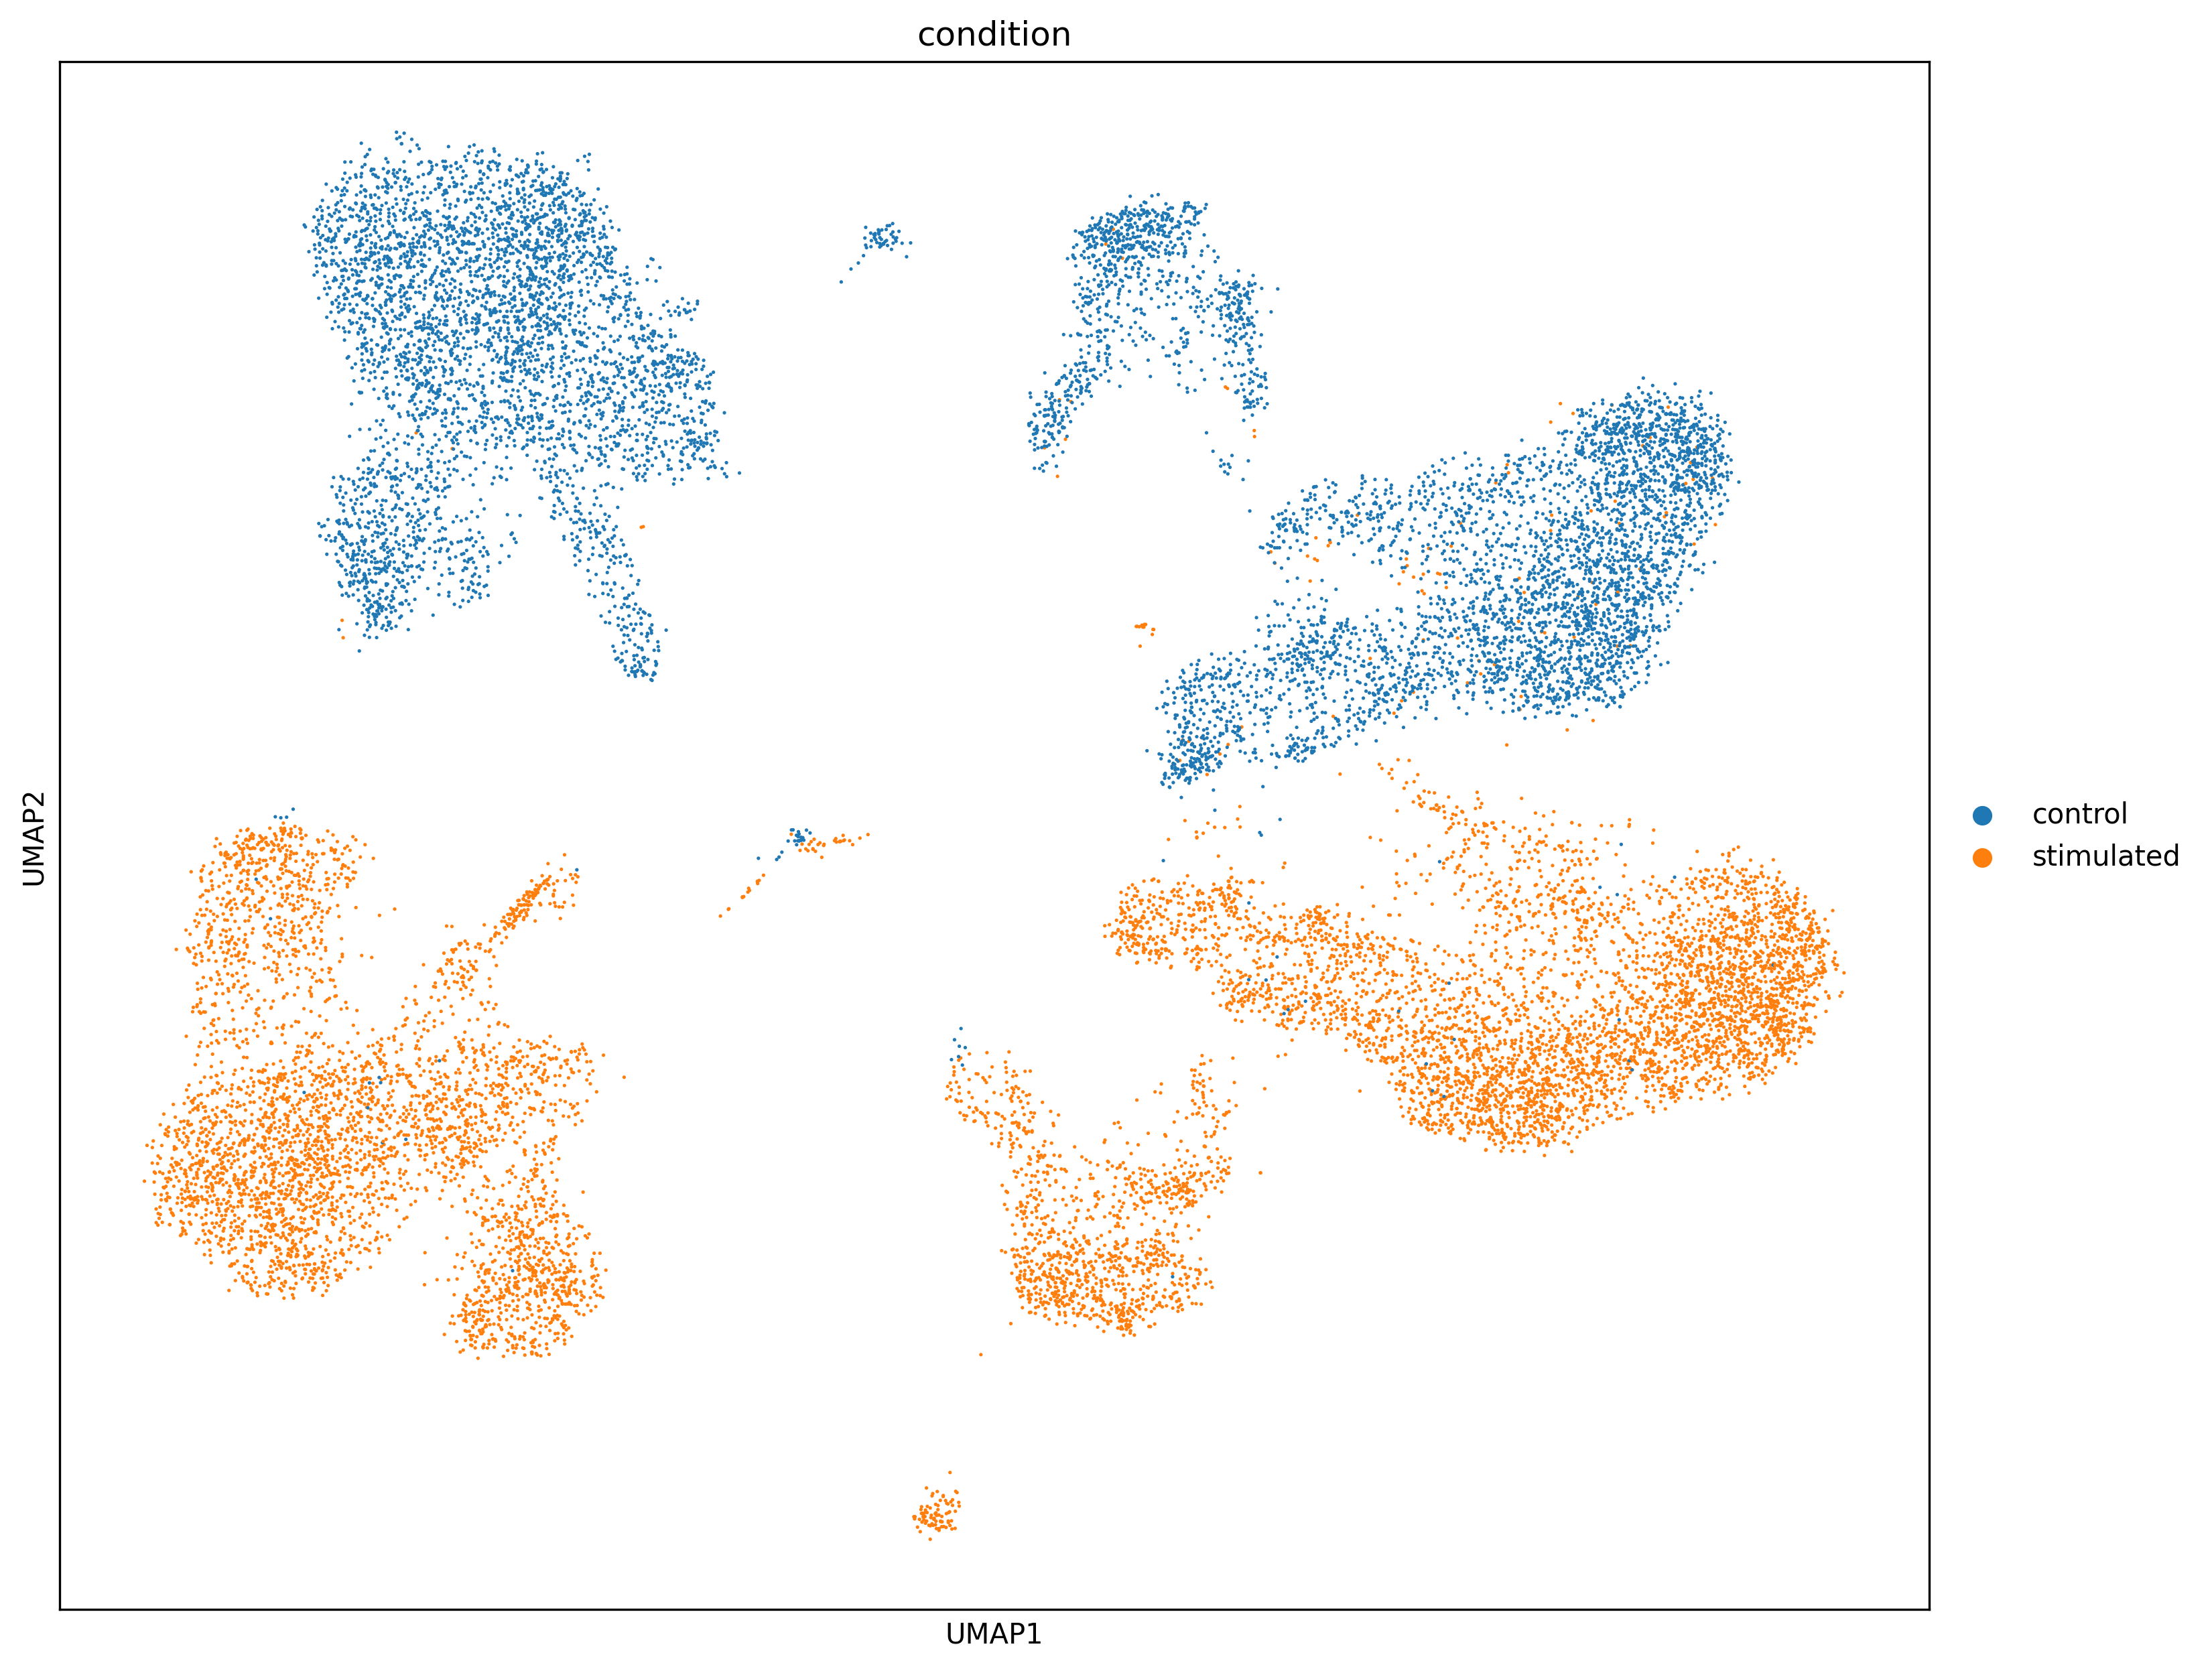
\includegraphics[width=.95\textwidth]{figures/pbmc_condtion_umap.png}
        \caption{}
        \label{fig:figure2}
    \end{subfigure}
    \hfill
    \begin{subfigure}[b]{\textwidth}
        \centering
        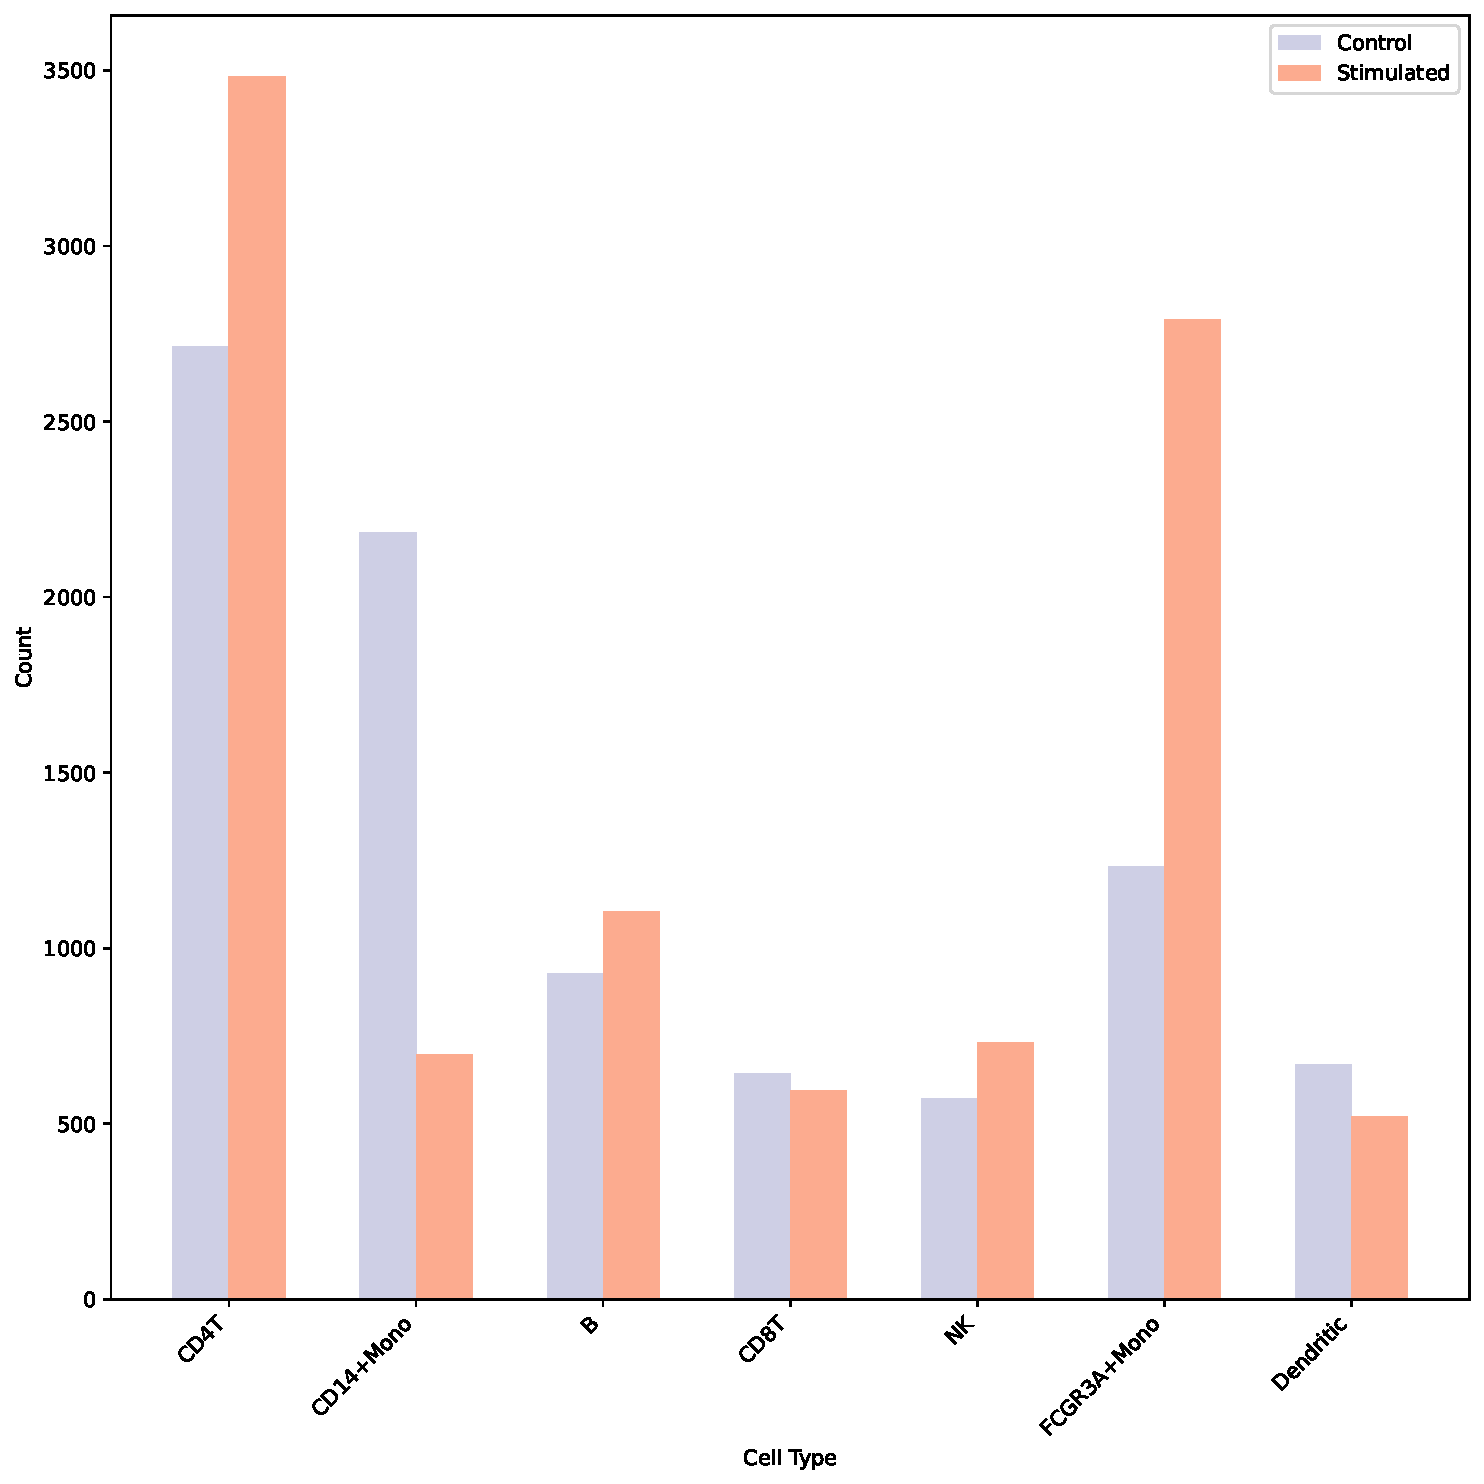
\includegraphics[width=.9\textwidth]{figures/pbmc_counts.pdf}
        \caption{}
        \label{fig:figure3}
    \end{subfigure}
    \caption{PBMC overview}
    \label{fig:combined}
\end{figure}

\clearpage

\begin{figure}
    \centering
    \begin{minipage}{0.4\textwidth}
        \centering
        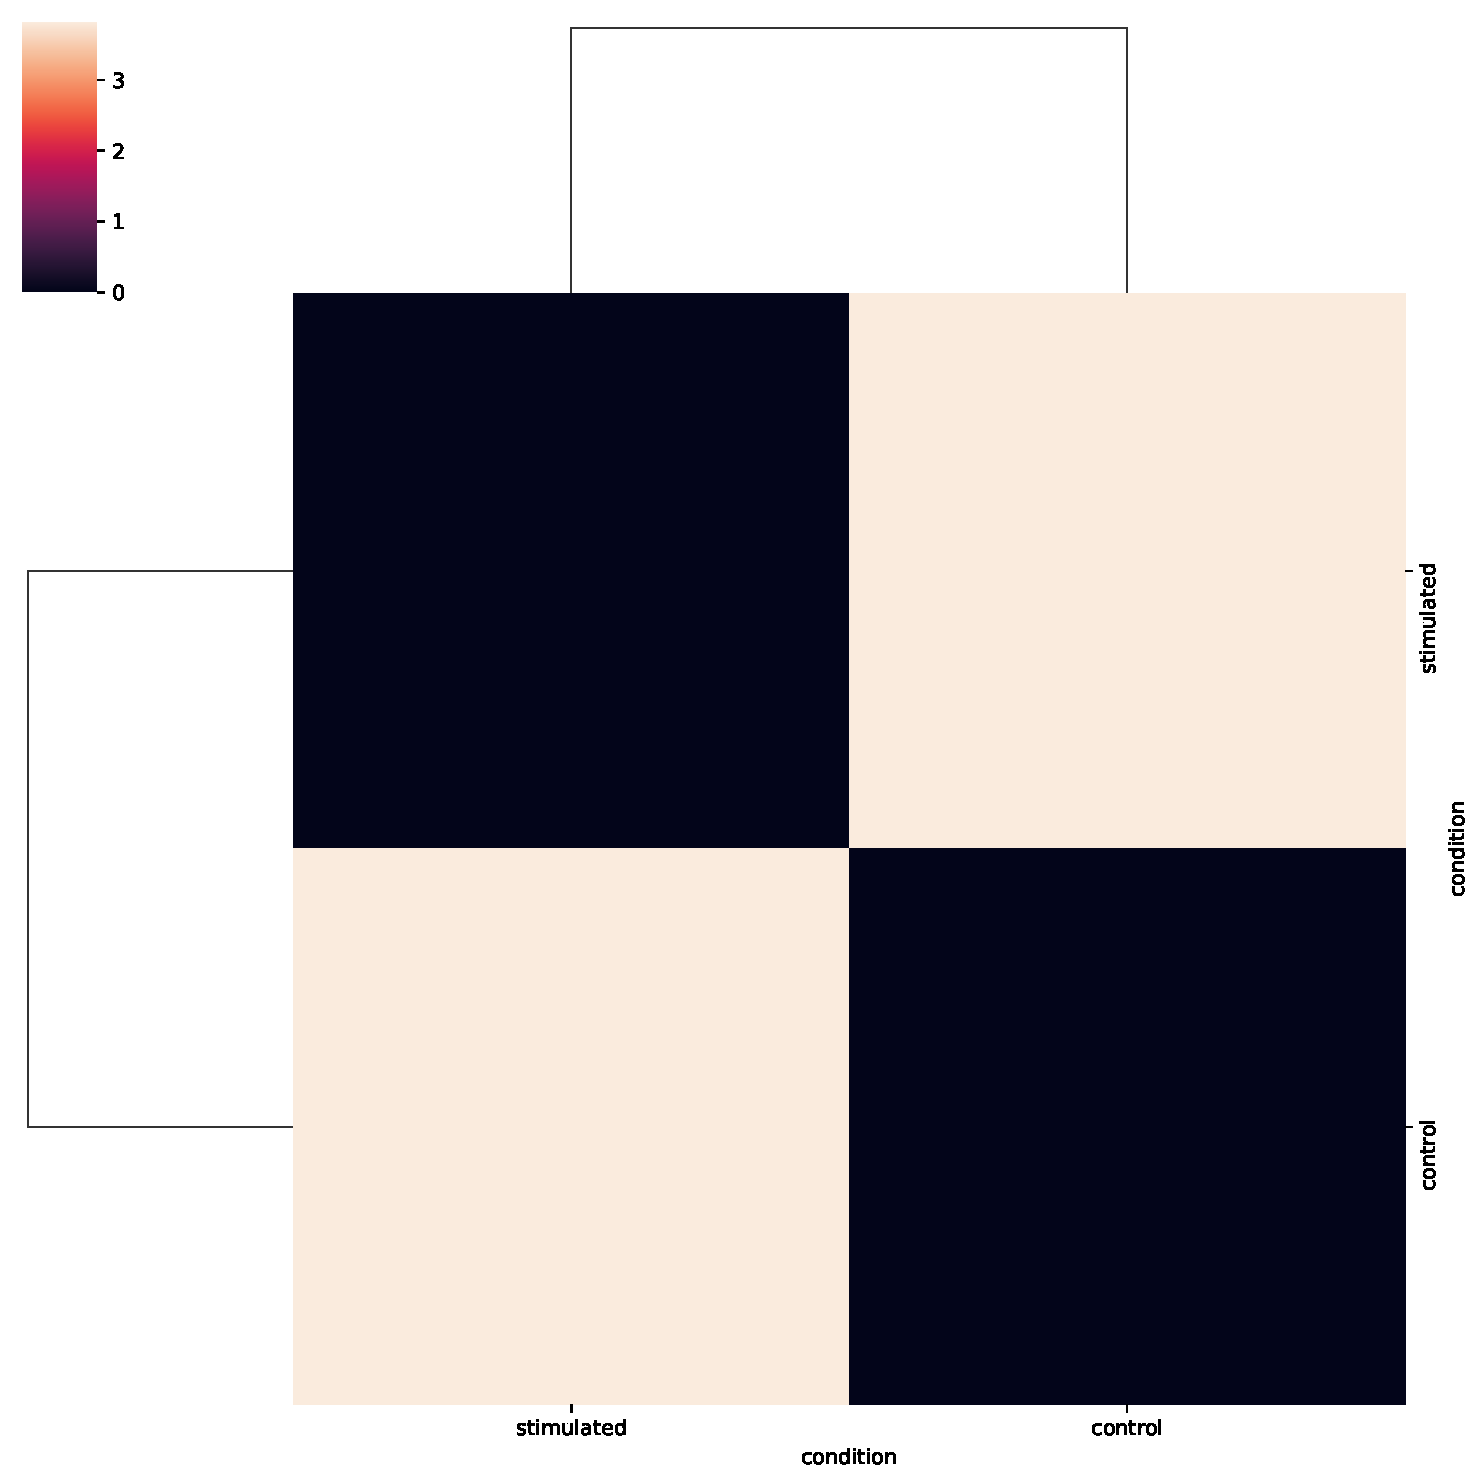
\includegraphics[width=\textwidth]{figures/pbmc_condition_edistance_clustermap.pdf}
        \caption{E-distance}
    \end{minipage} \hfill
    \begin{minipage}{0.4\textwidth}
        \centering
        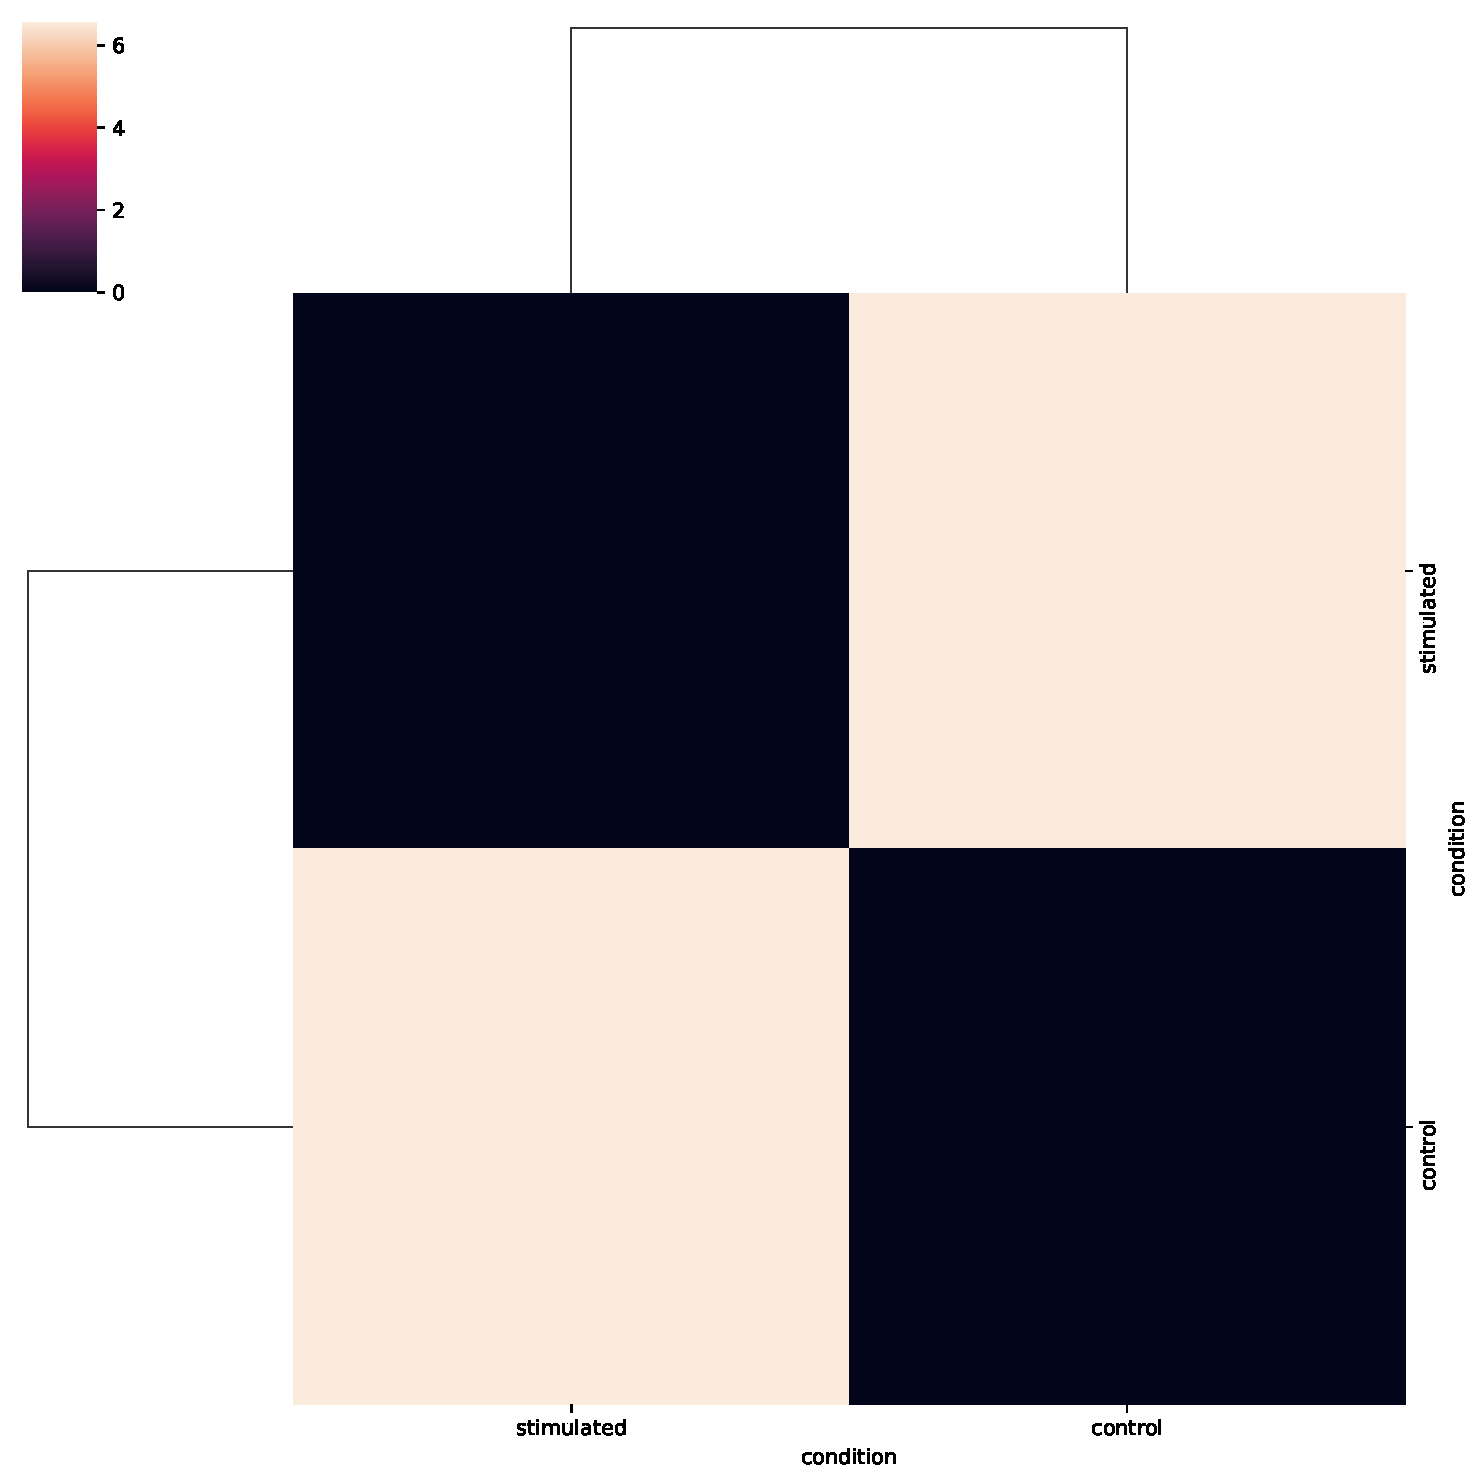
\includegraphics[width=\textwidth]{figures/pbmc_condition_euclidean_clustermap.pdf}
        \caption{Euclidean}
    \end{minipage}
    \vskip\baselineskip

    \begin{minipage}{0.4\textwidth}
        \centering
        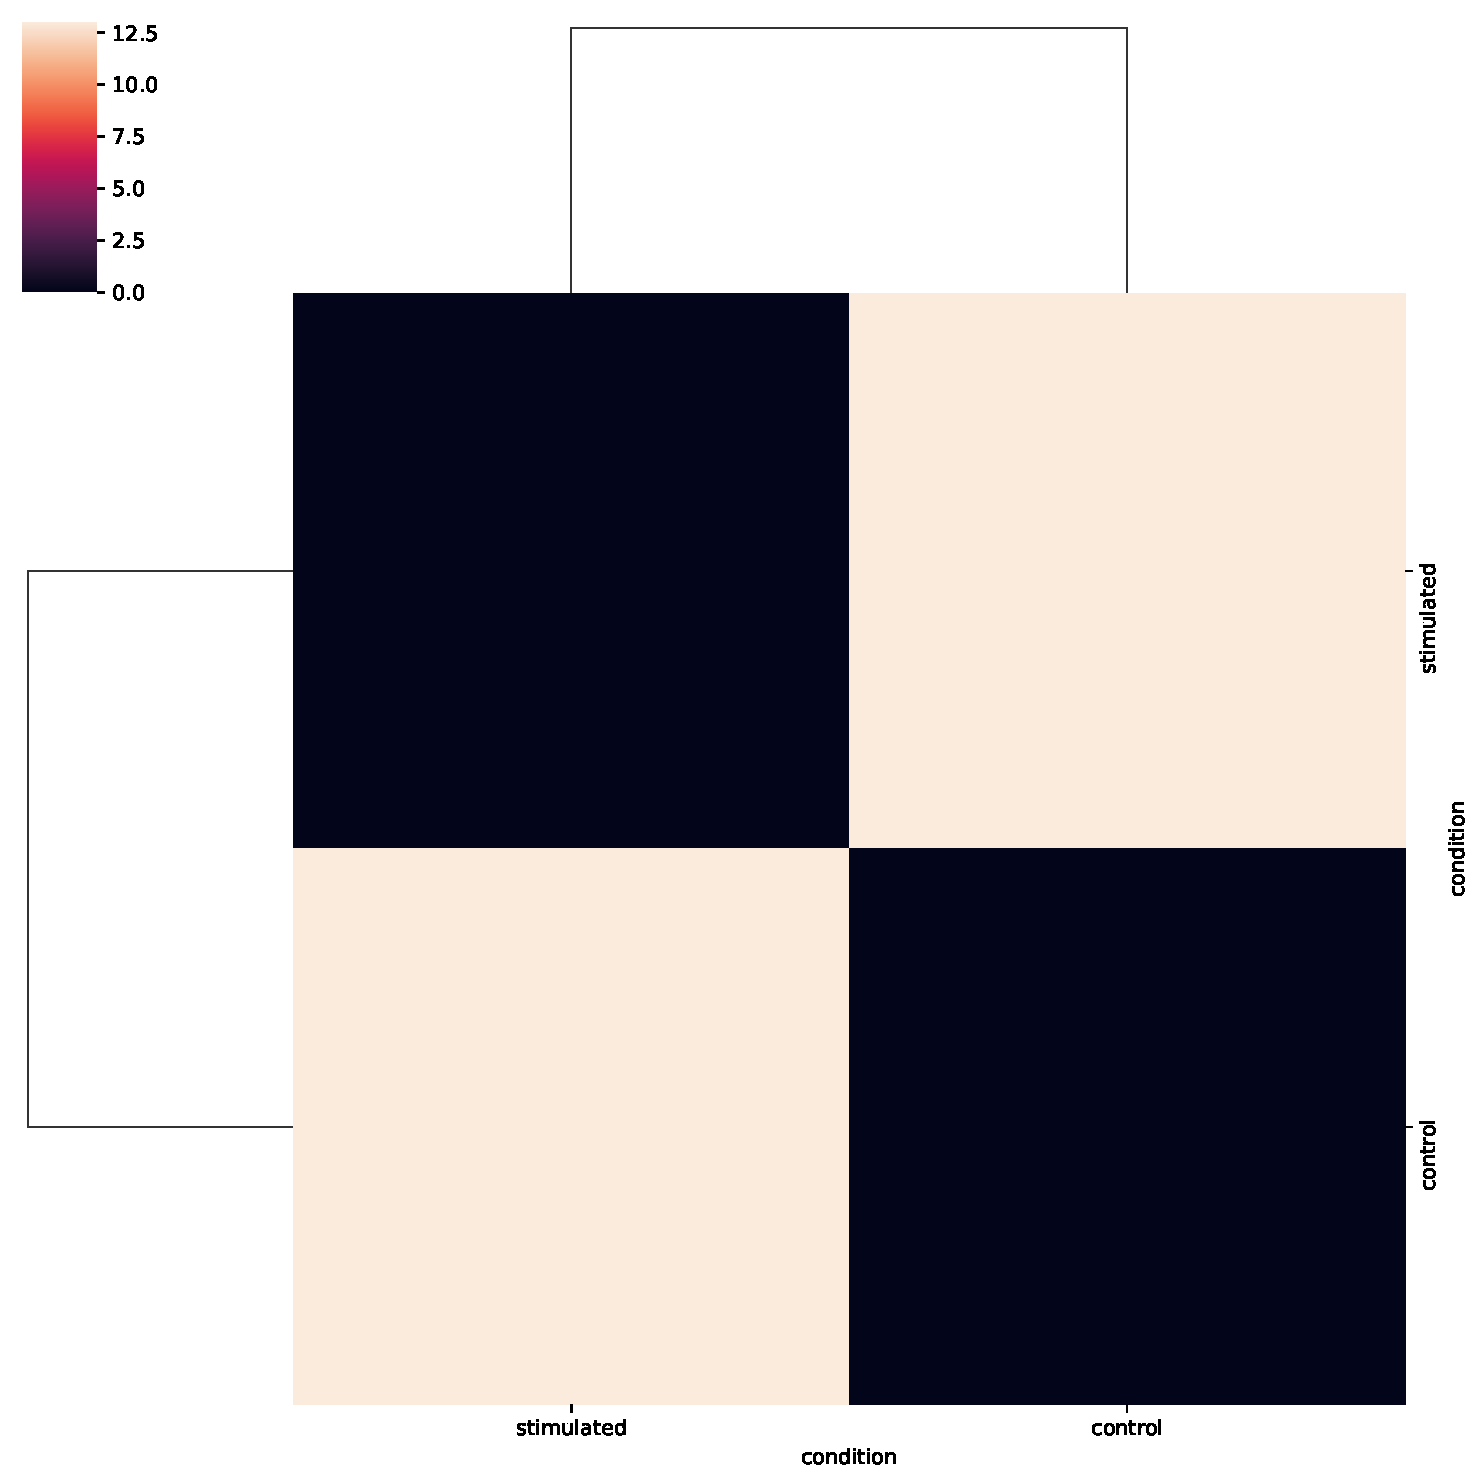
\includegraphics[width=\textwidth]{figures/pbmc_condition_mean_pairwise_clustermap.pdf}
        \caption{Mean pairwise}
    \end{minipage} \hfill
    \begin{minipage}{0.4\textwidth}
        \centering
        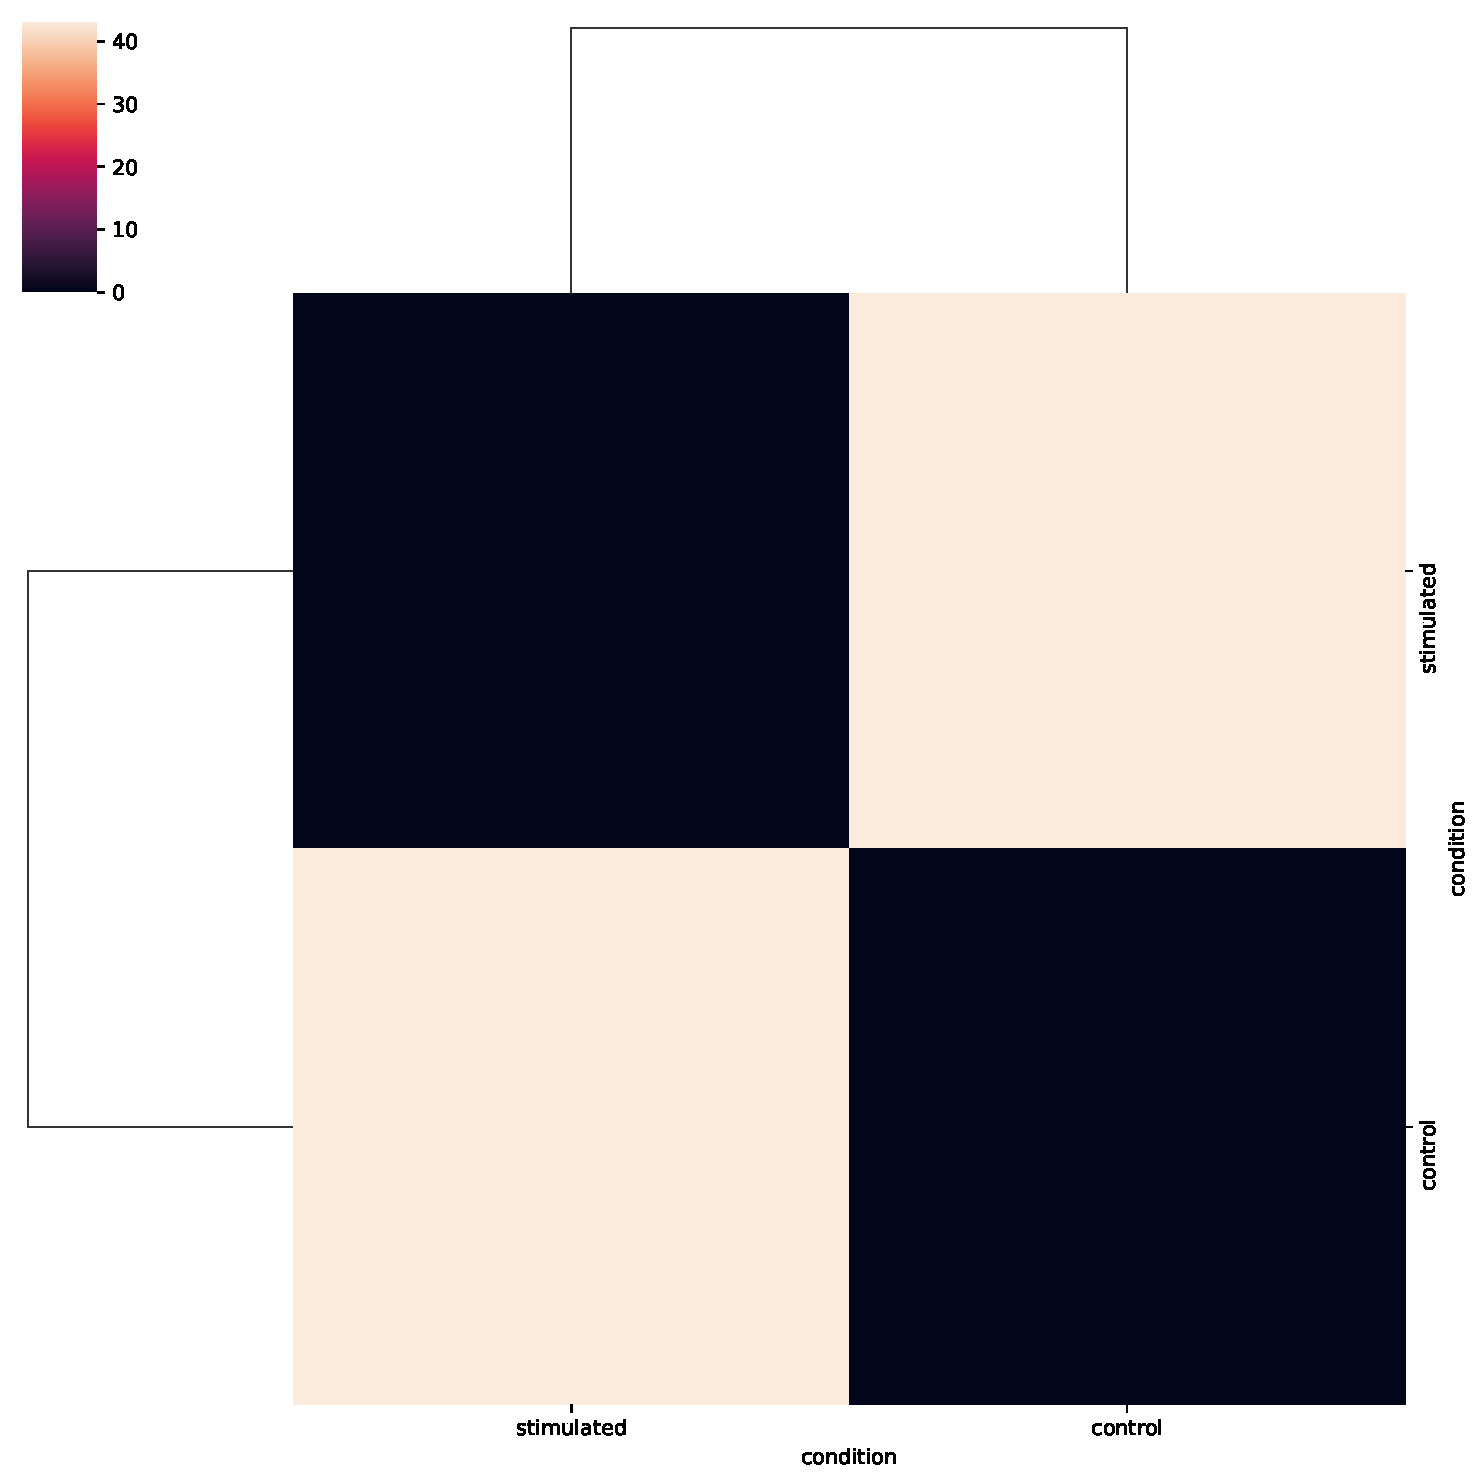
\includegraphics[width=\textwidth]{figures/pbmc_condition_mmd_clustermap.pdf}
        \caption{MMD}
    \end{minipage}
    \vskip\baselineskip

    \begin{minipage}{0.4\textwidth}
        \centering
        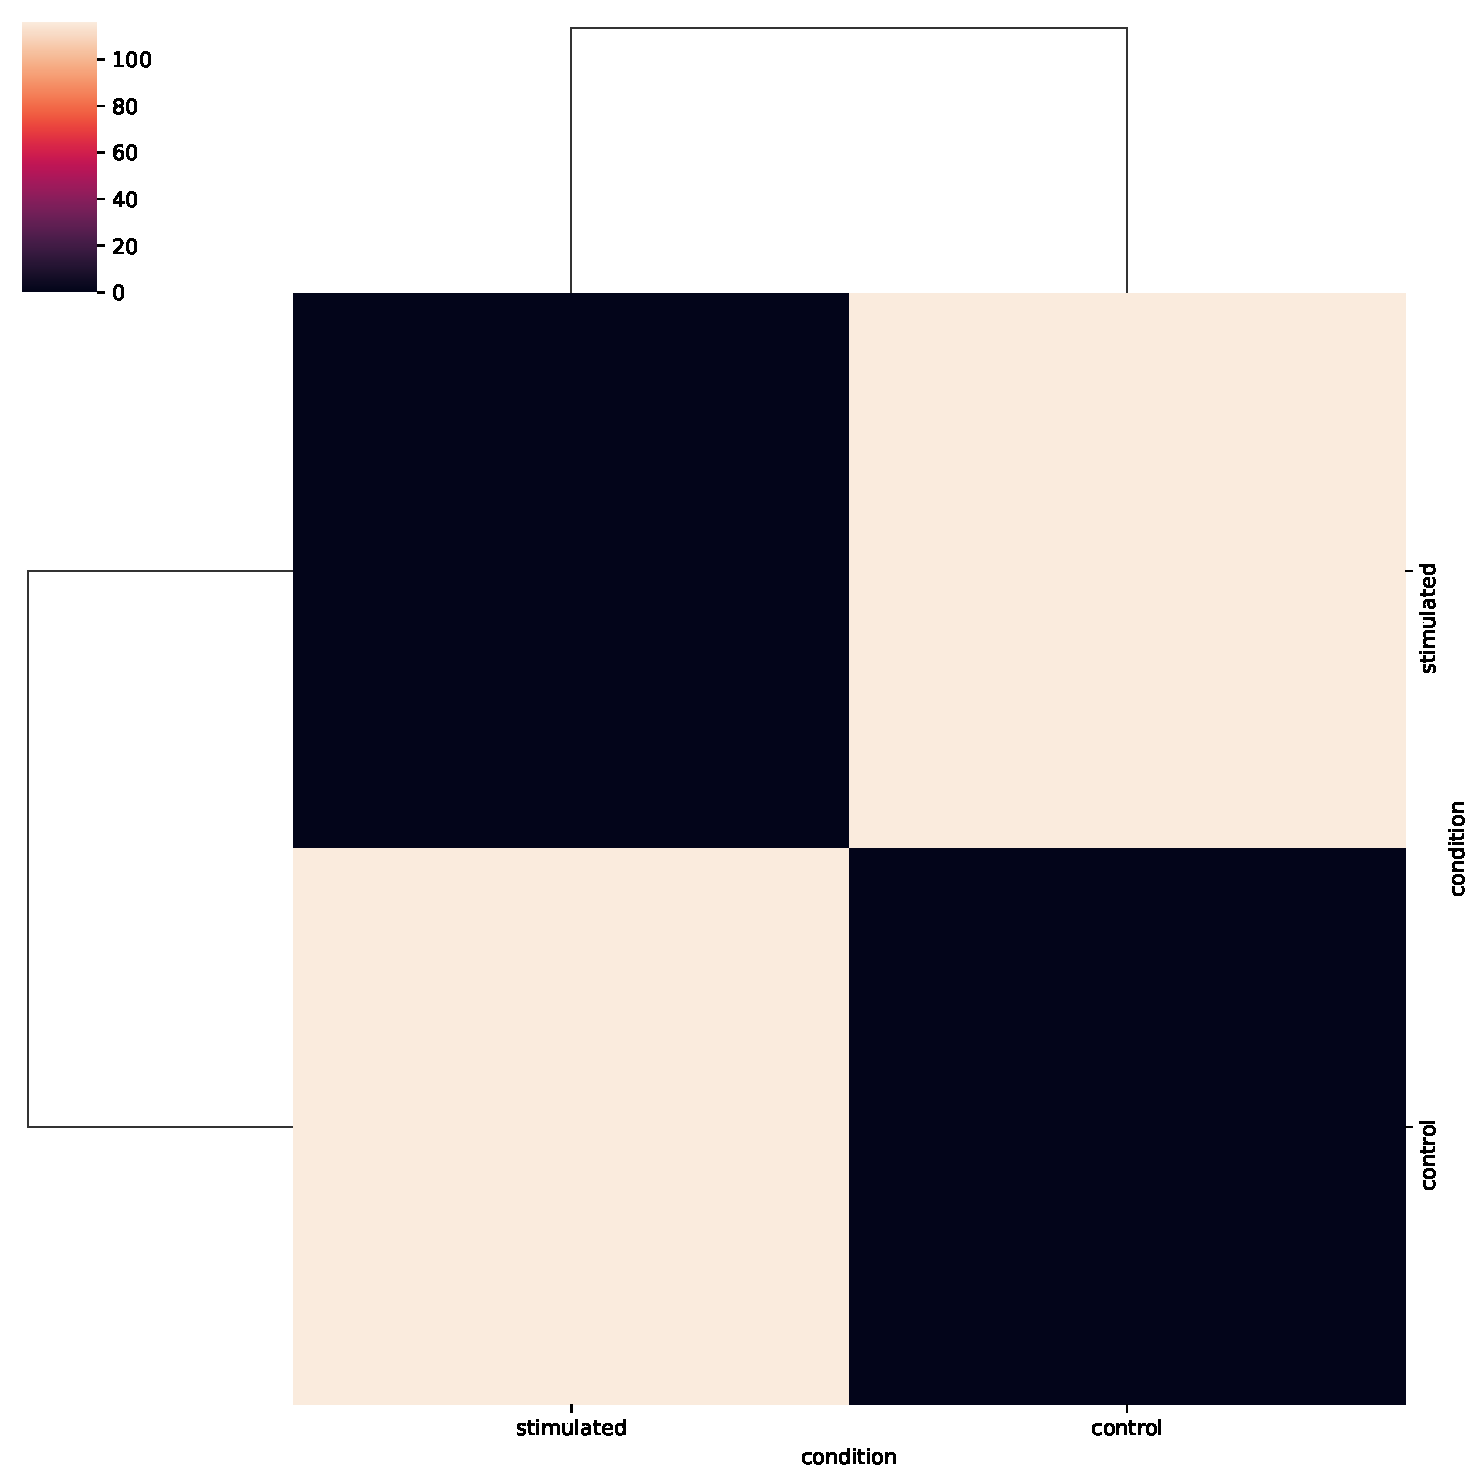
\includegraphics[width=\textwidth]{figures/pbmc_condition_wasserstein_clustermap.pdf}
        \caption{Wasserstein}
    \end{minipage}
    \caption{Distance metrics per condition}
\end{figure}

\clearpage


\begin{figure}
    \centering
    \begin{minipage}{0.4\textwidth}
        \centering
        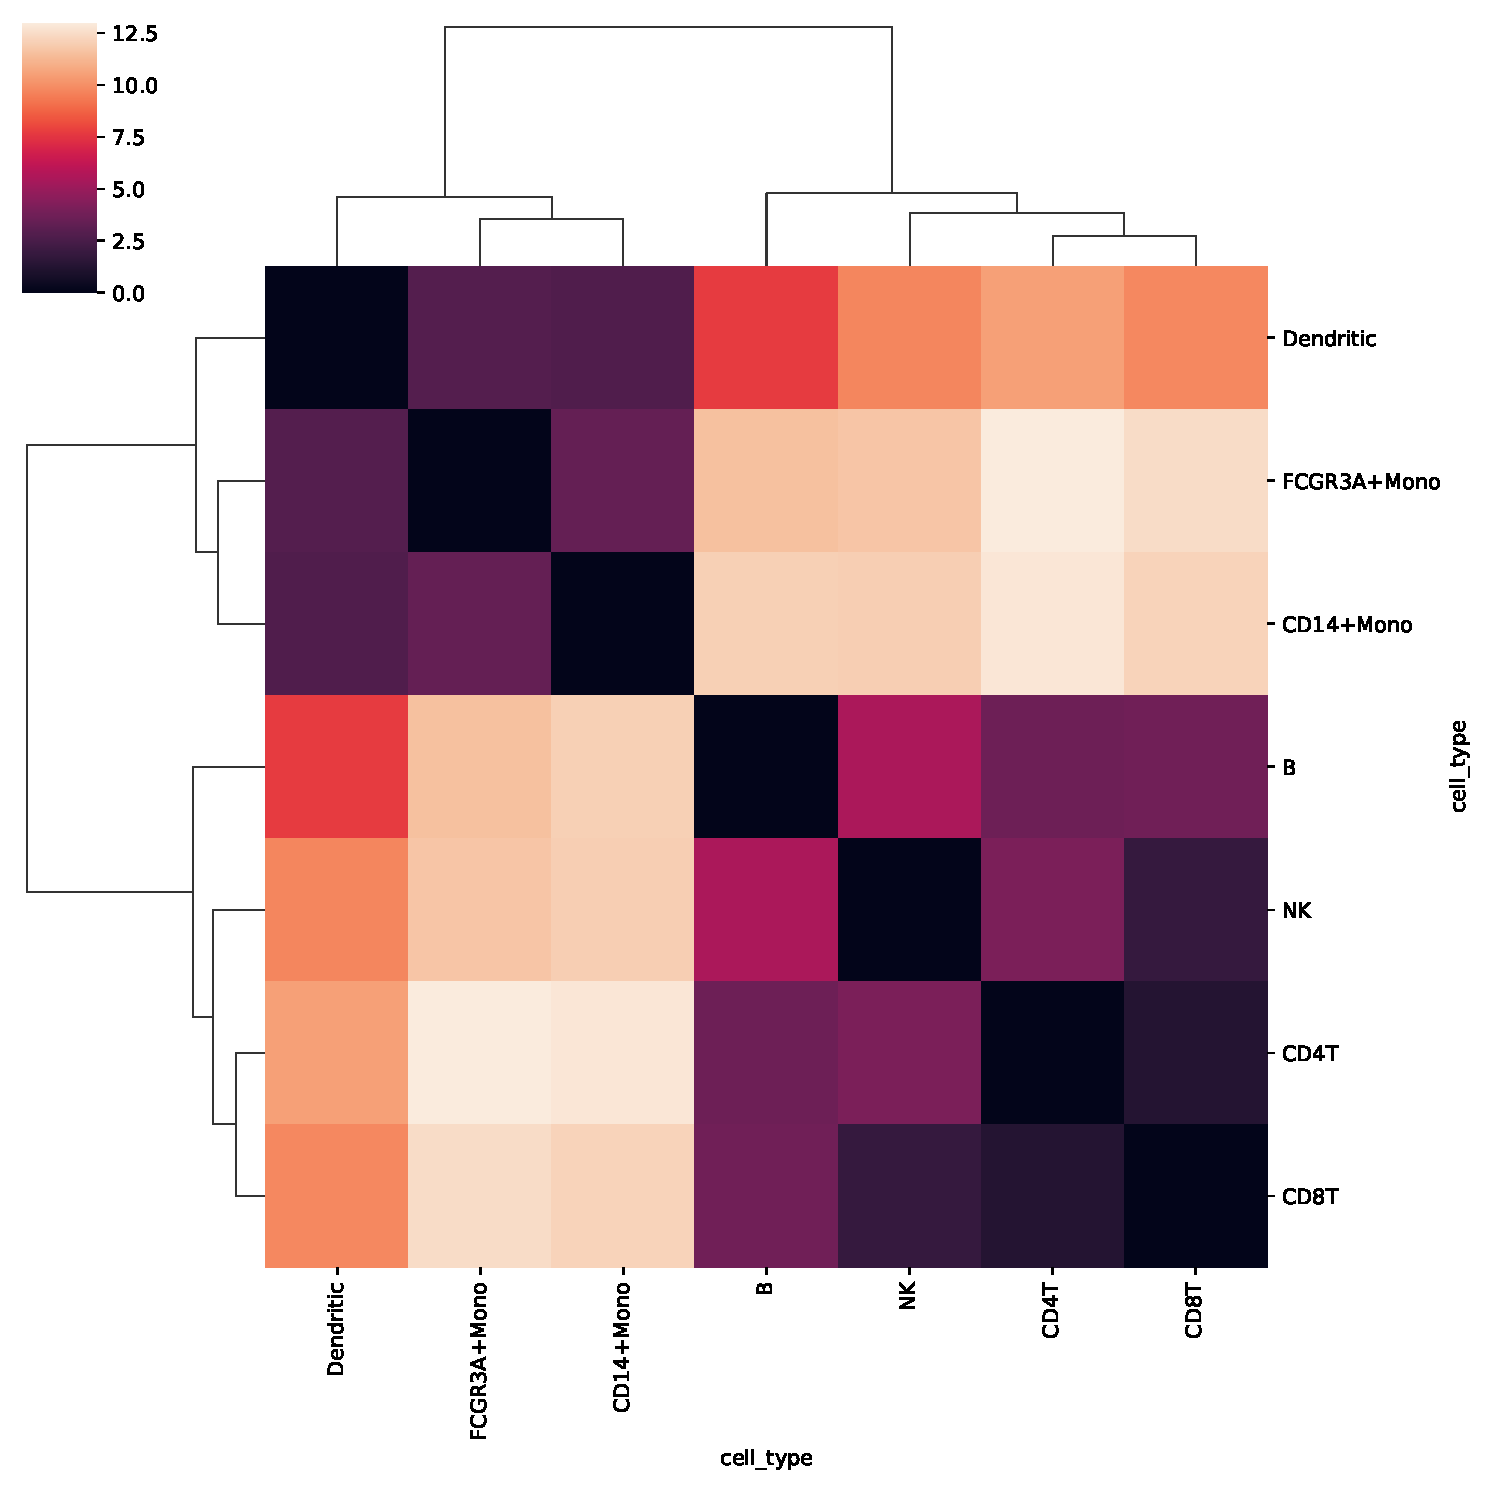
\includegraphics[width=\textwidth]{figures/pbmc_cell_type_edistance_clustermap.pdf}
        \caption{E-distance}
    \end{minipage} \hfill
    \begin{minipage}{0.4\textwidth}
        \centering
        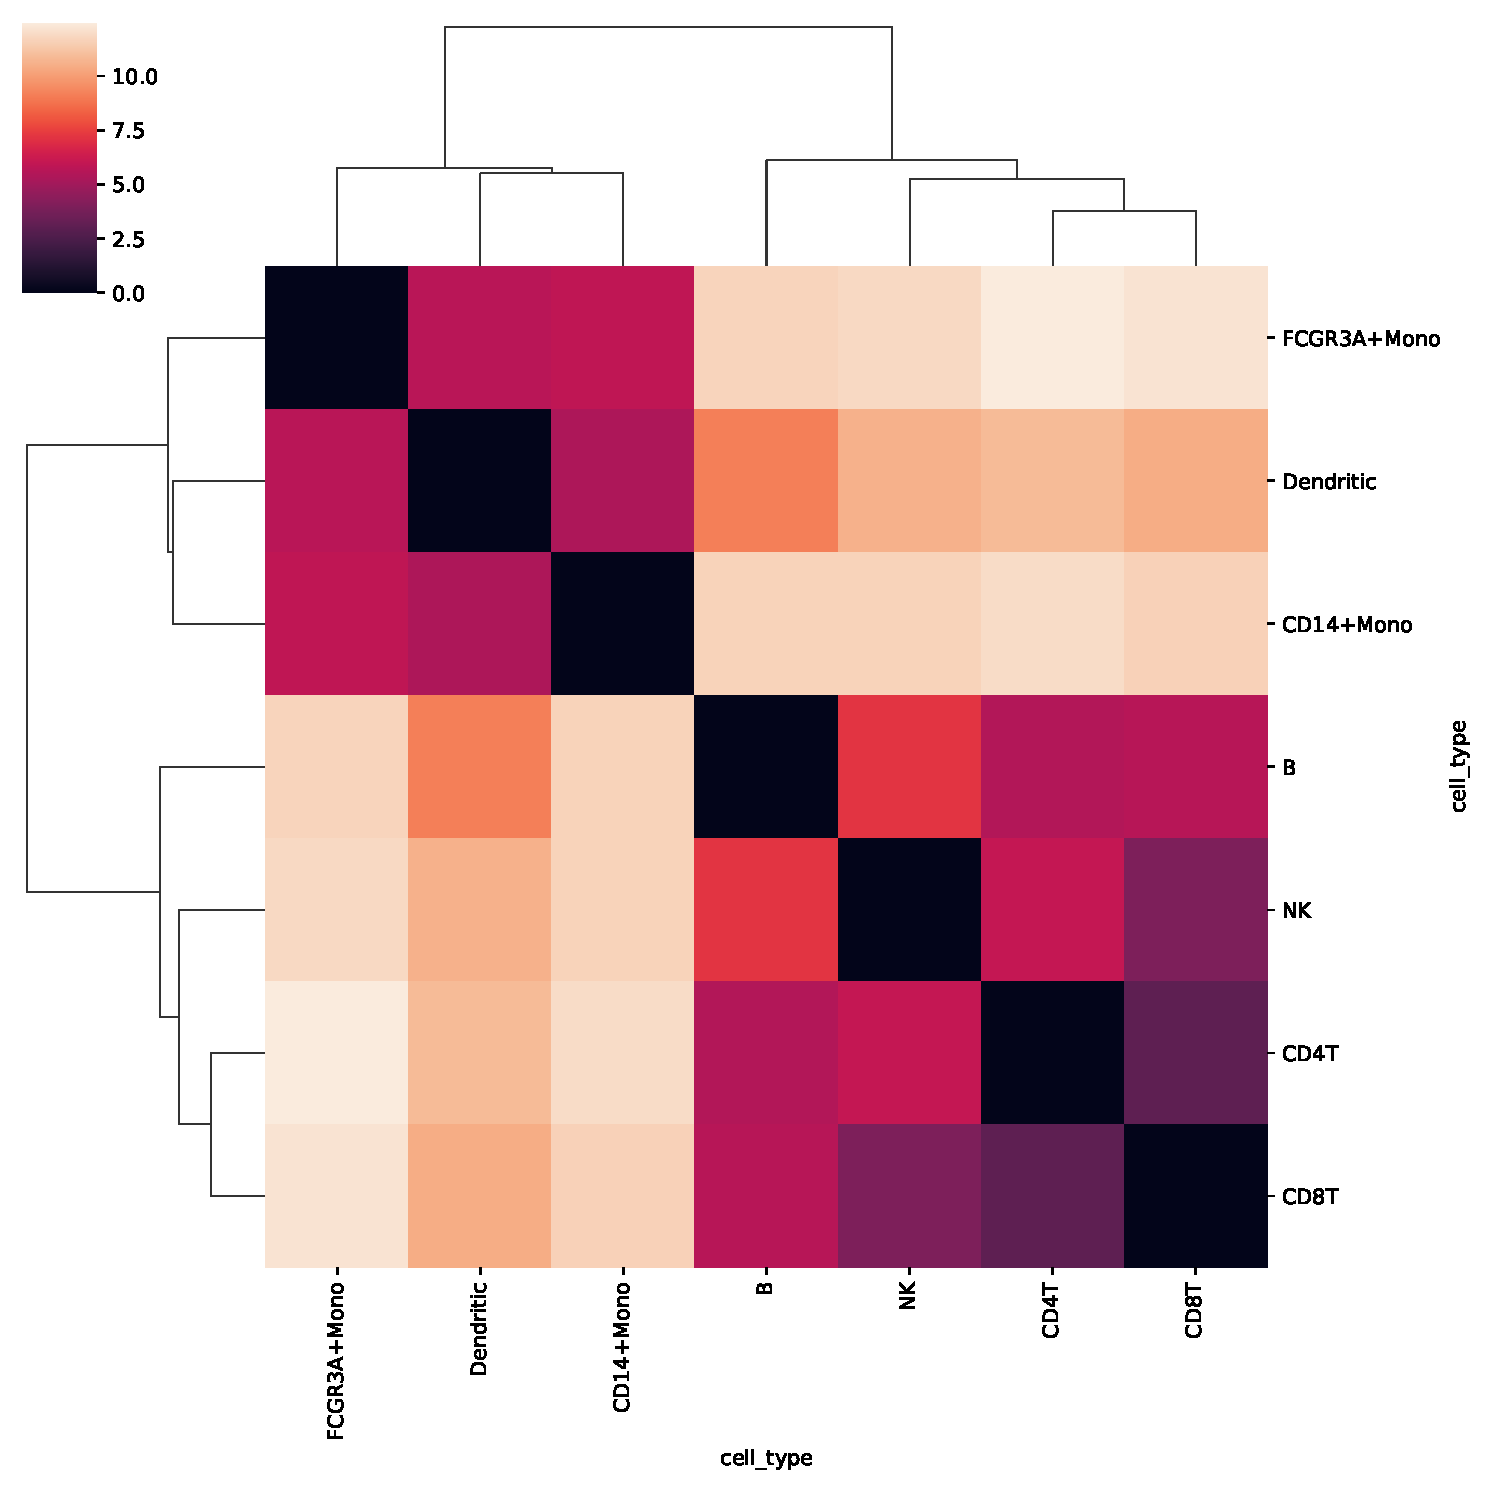
\includegraphics[width=\textwidth]{figures/pbmc_cell_type_euclidean_clustermap.pdf}
        \caption{Euclidean}
    \end{minipage}
    \vskip\baselineskip

    \begin{minipage}{0.4\textwidth}
        \centering
        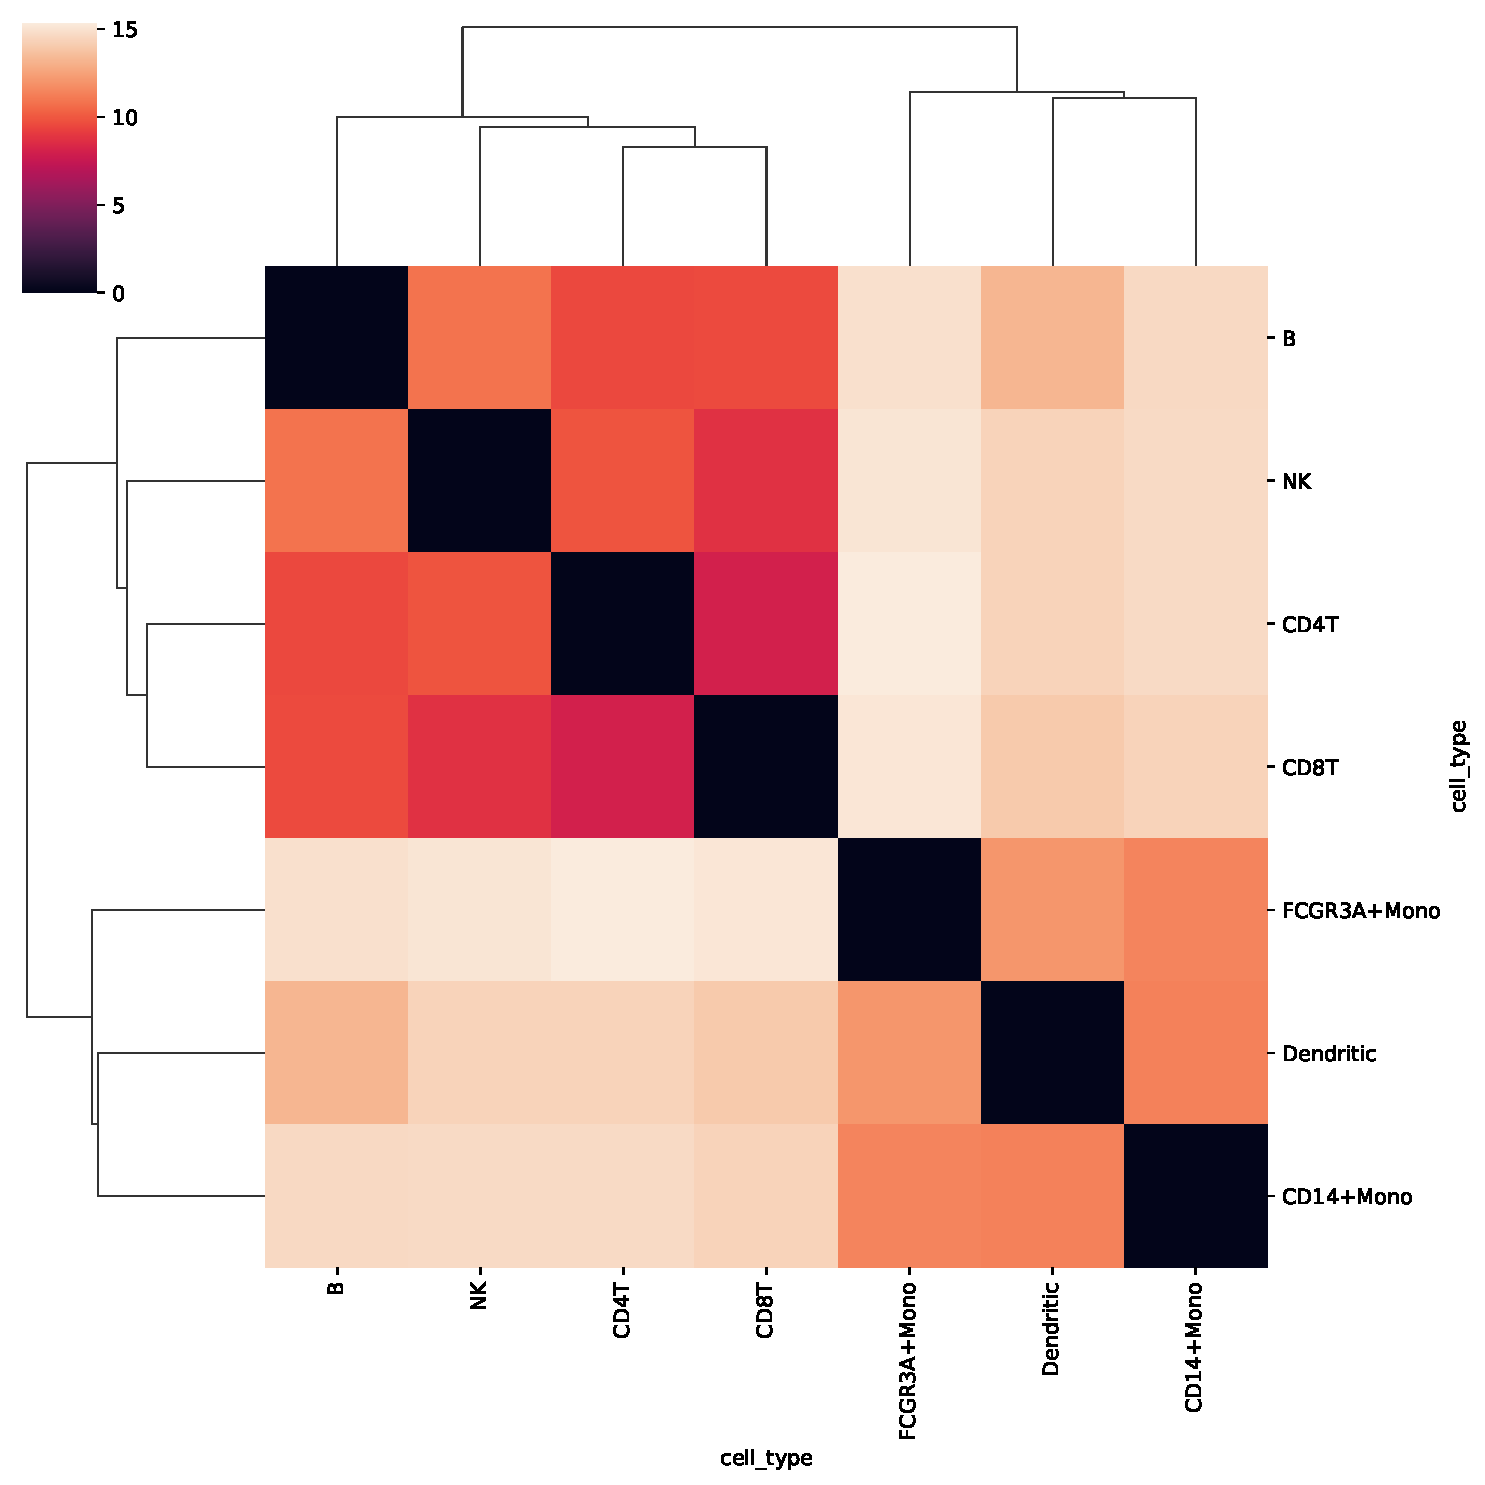
\includegraphics[width=\textwidth]{figures/pbmc_cell_type_mean_pairwise_clustermap.pdf}
        \caption{Mean pairwise}
    \end{minipage} \hfill
    \begin{minipage}{0.4\textwidth}
        \centering
        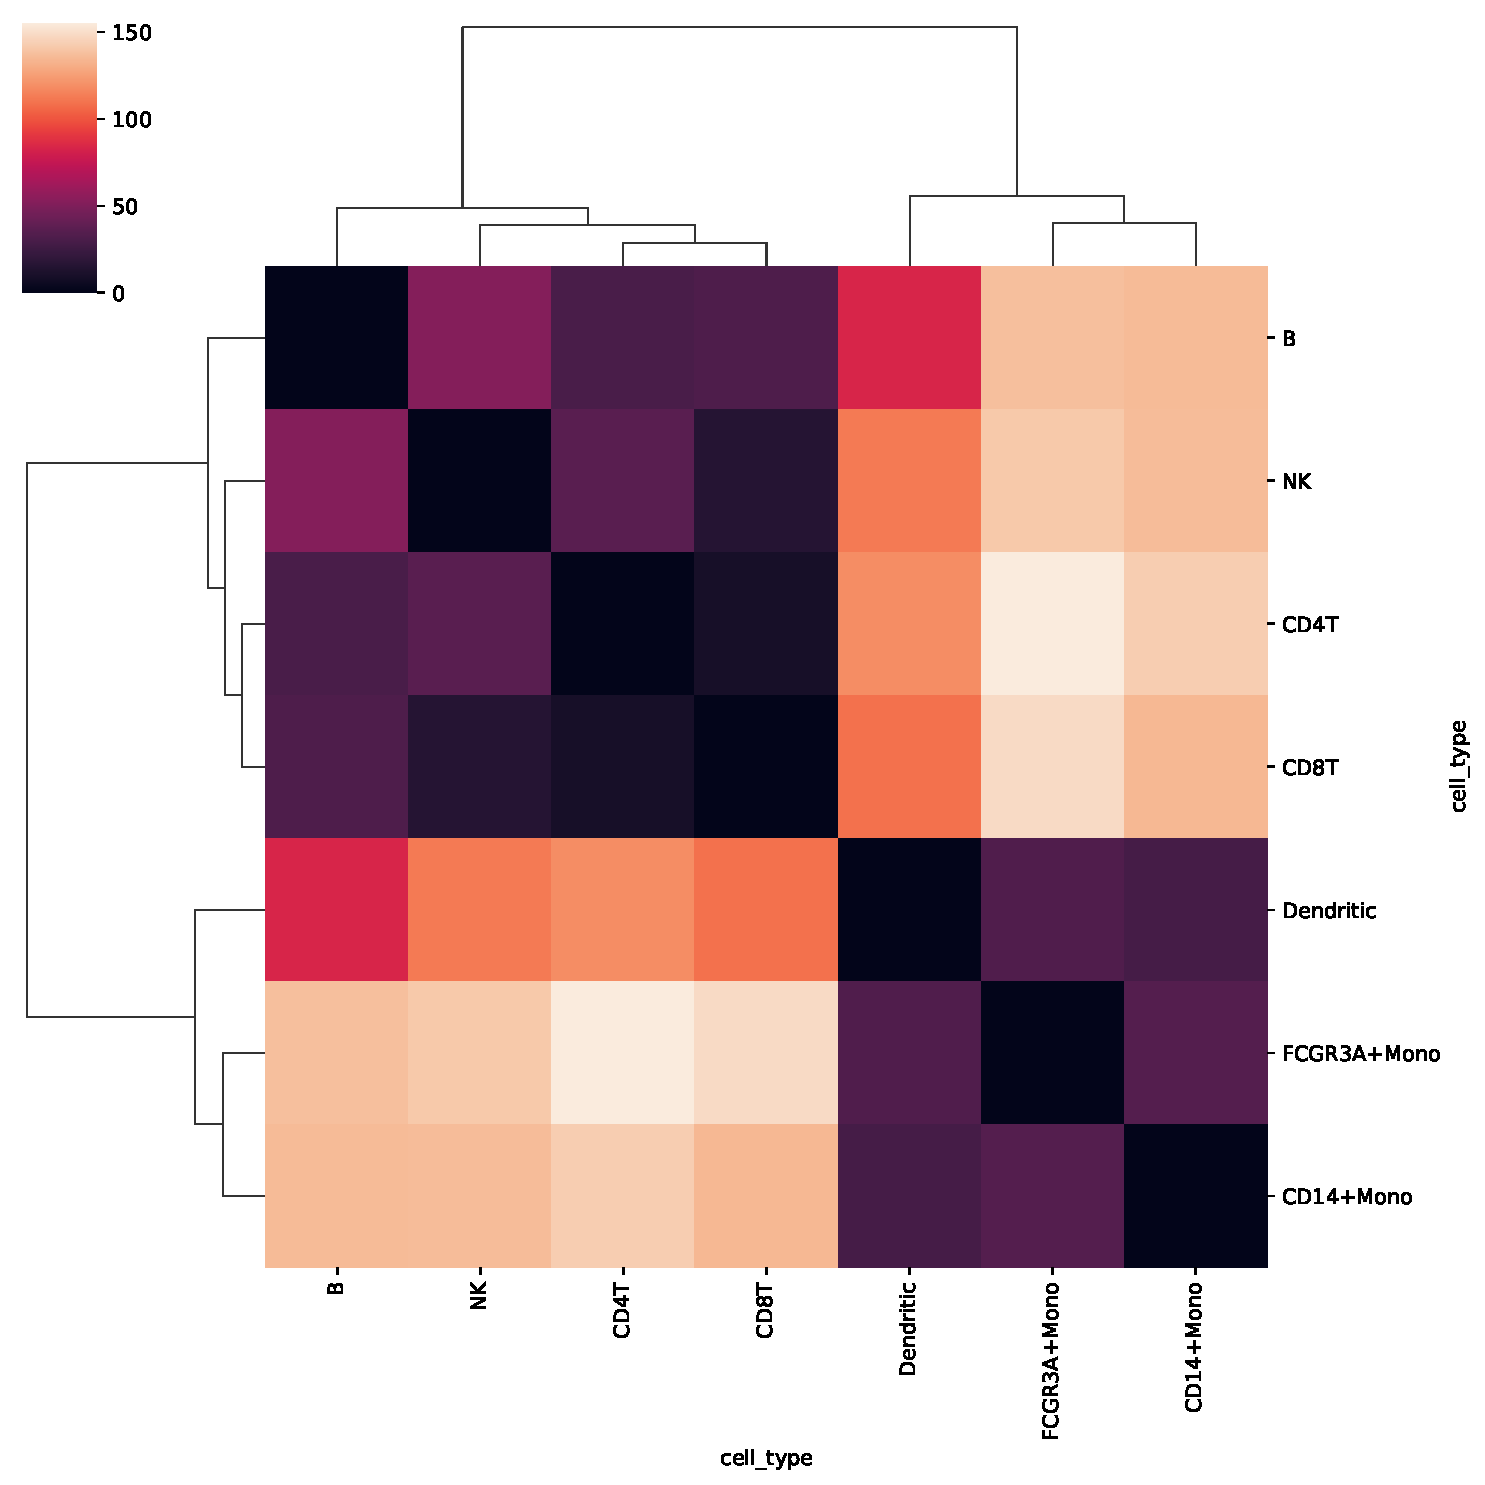
\includegraphics[width=\textwidth]{figures/pbmc_cell_type_mmd_clustermap.pdf}
        \caption{MMD}
    \end{minipage}
    \vskip\baselineskip

    \begin{minipage}{0.4\textwidth}
        \centering
        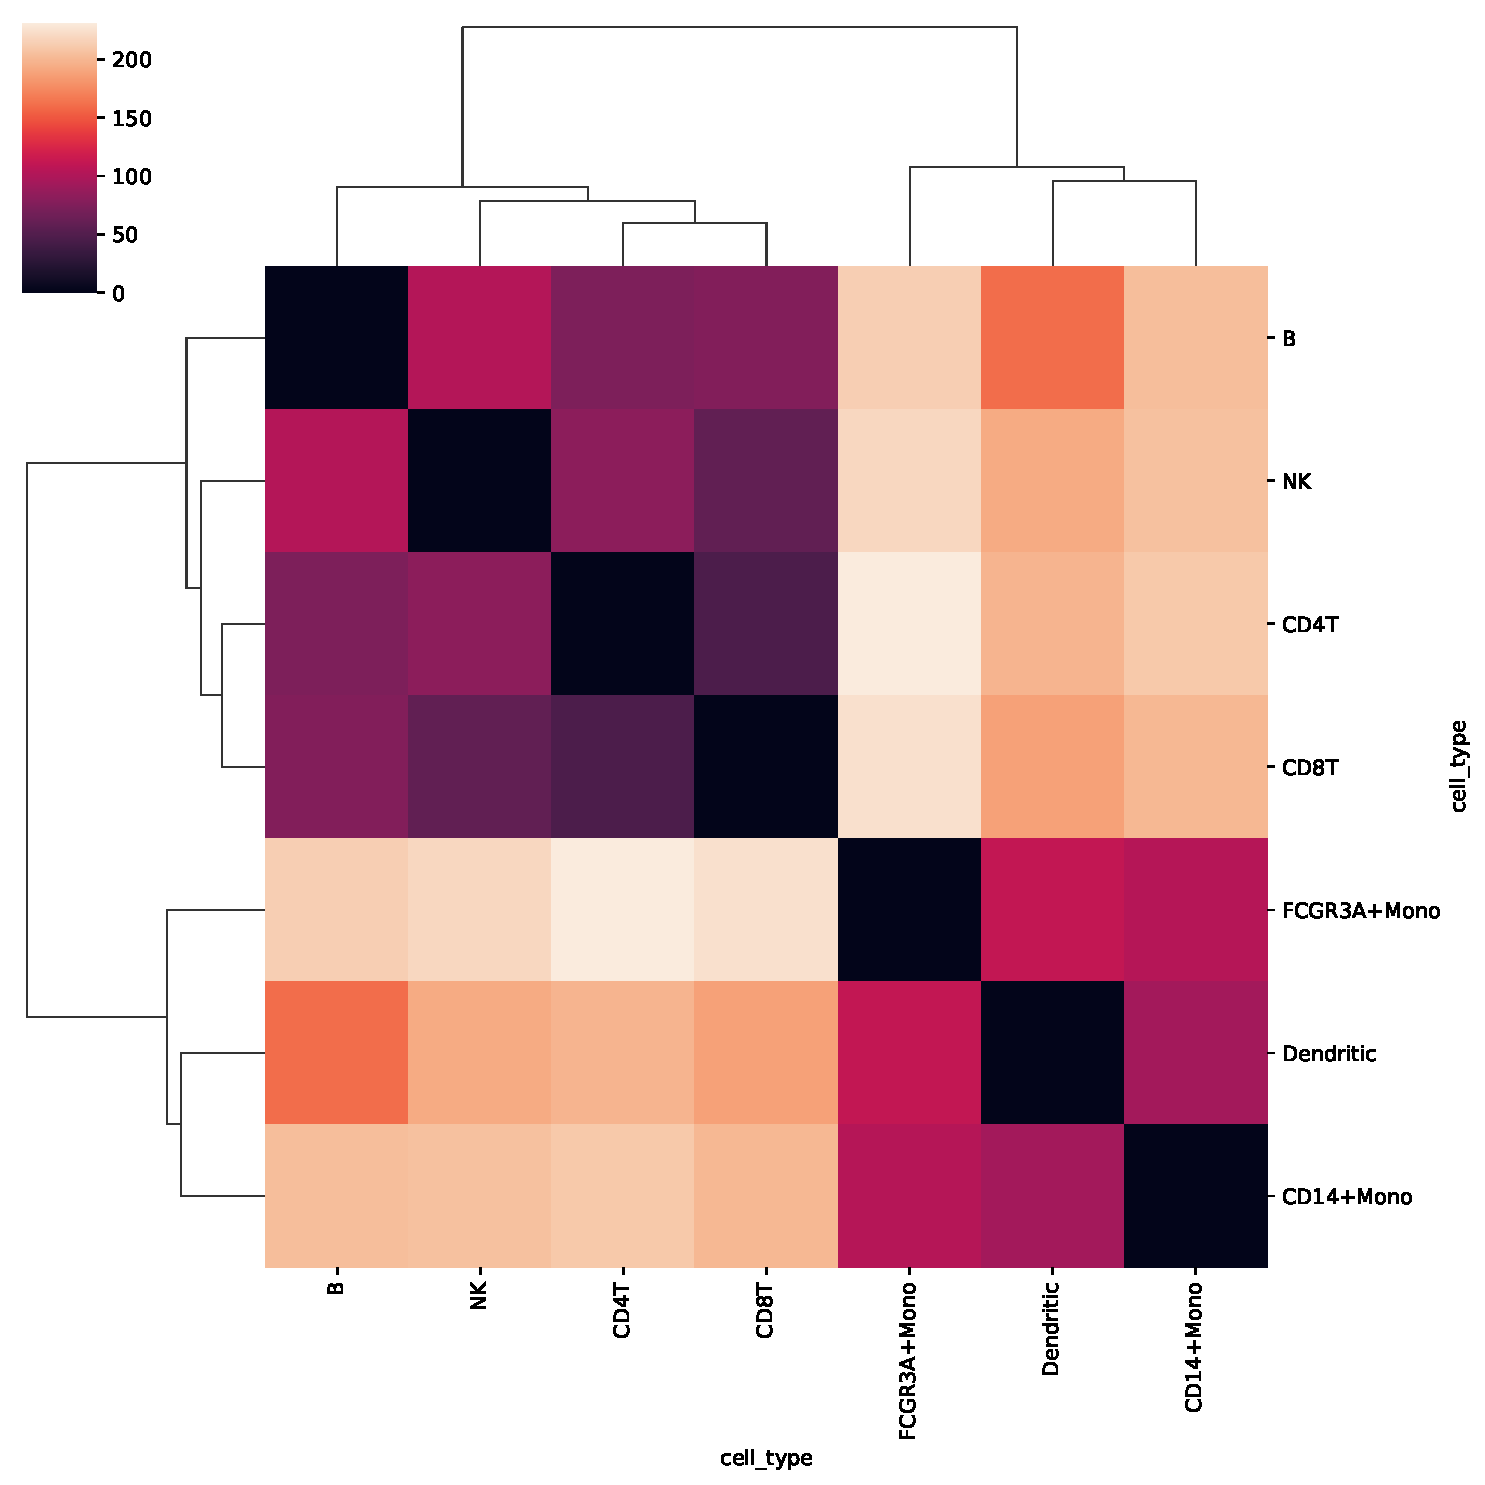
\includegraphics[width=\textwidth]{figures/pbmc_cell_type_wasserstein_clustermap.pdf}
        \caption{Wasserstein}
    \end{minipage}
    \caption{Distance metrics per cell type}
\end{figure}

\clearpage


\section{Nault all cell types evaluation}

\subsection{Multiple doses}

\begin{figure}[h!]
    \centering
    \includegraphics[width=.8\textwidth]{figures/nault_umap_split_multiple.png}
\end{figure}

\begin{figure}[h!]
    \centering
    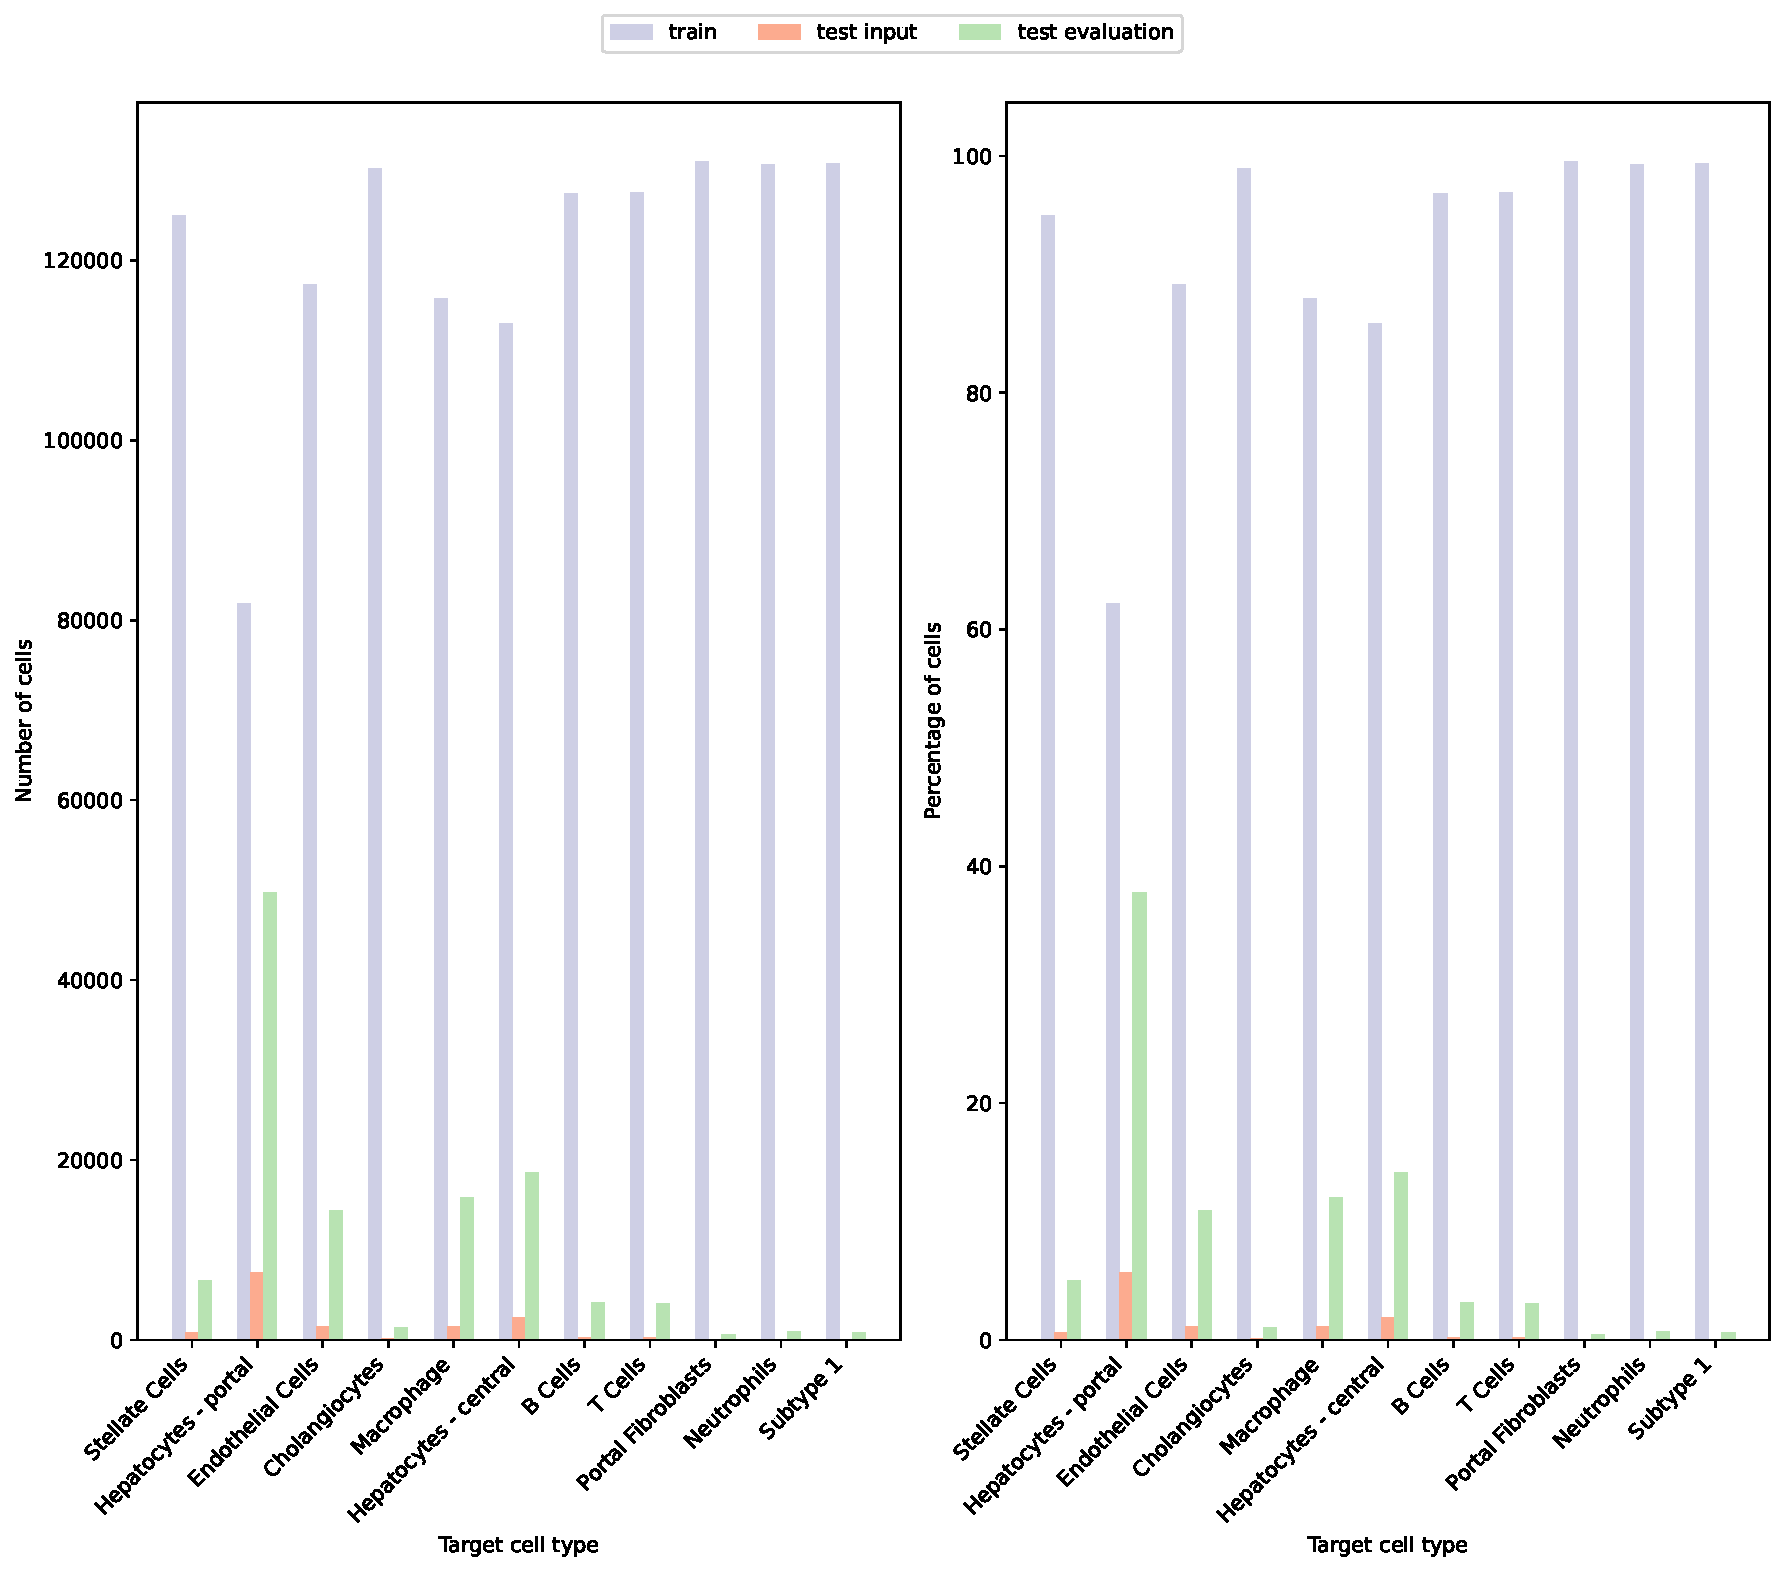
\includegraphics[width=.8\textwidth]{figures/nault_bars_split_multiple.pdf}
\end{figure}


\subsection{Single dose}


\begin{figure}[h!]
    \centering
    \includegraphics[width=.7\textwidth]{figures/nault_umap_split_30.png}
    \caption{Example of $30 \mu g/kg$}
\end{figure}

\begin{figure}[h!]
    \centering
    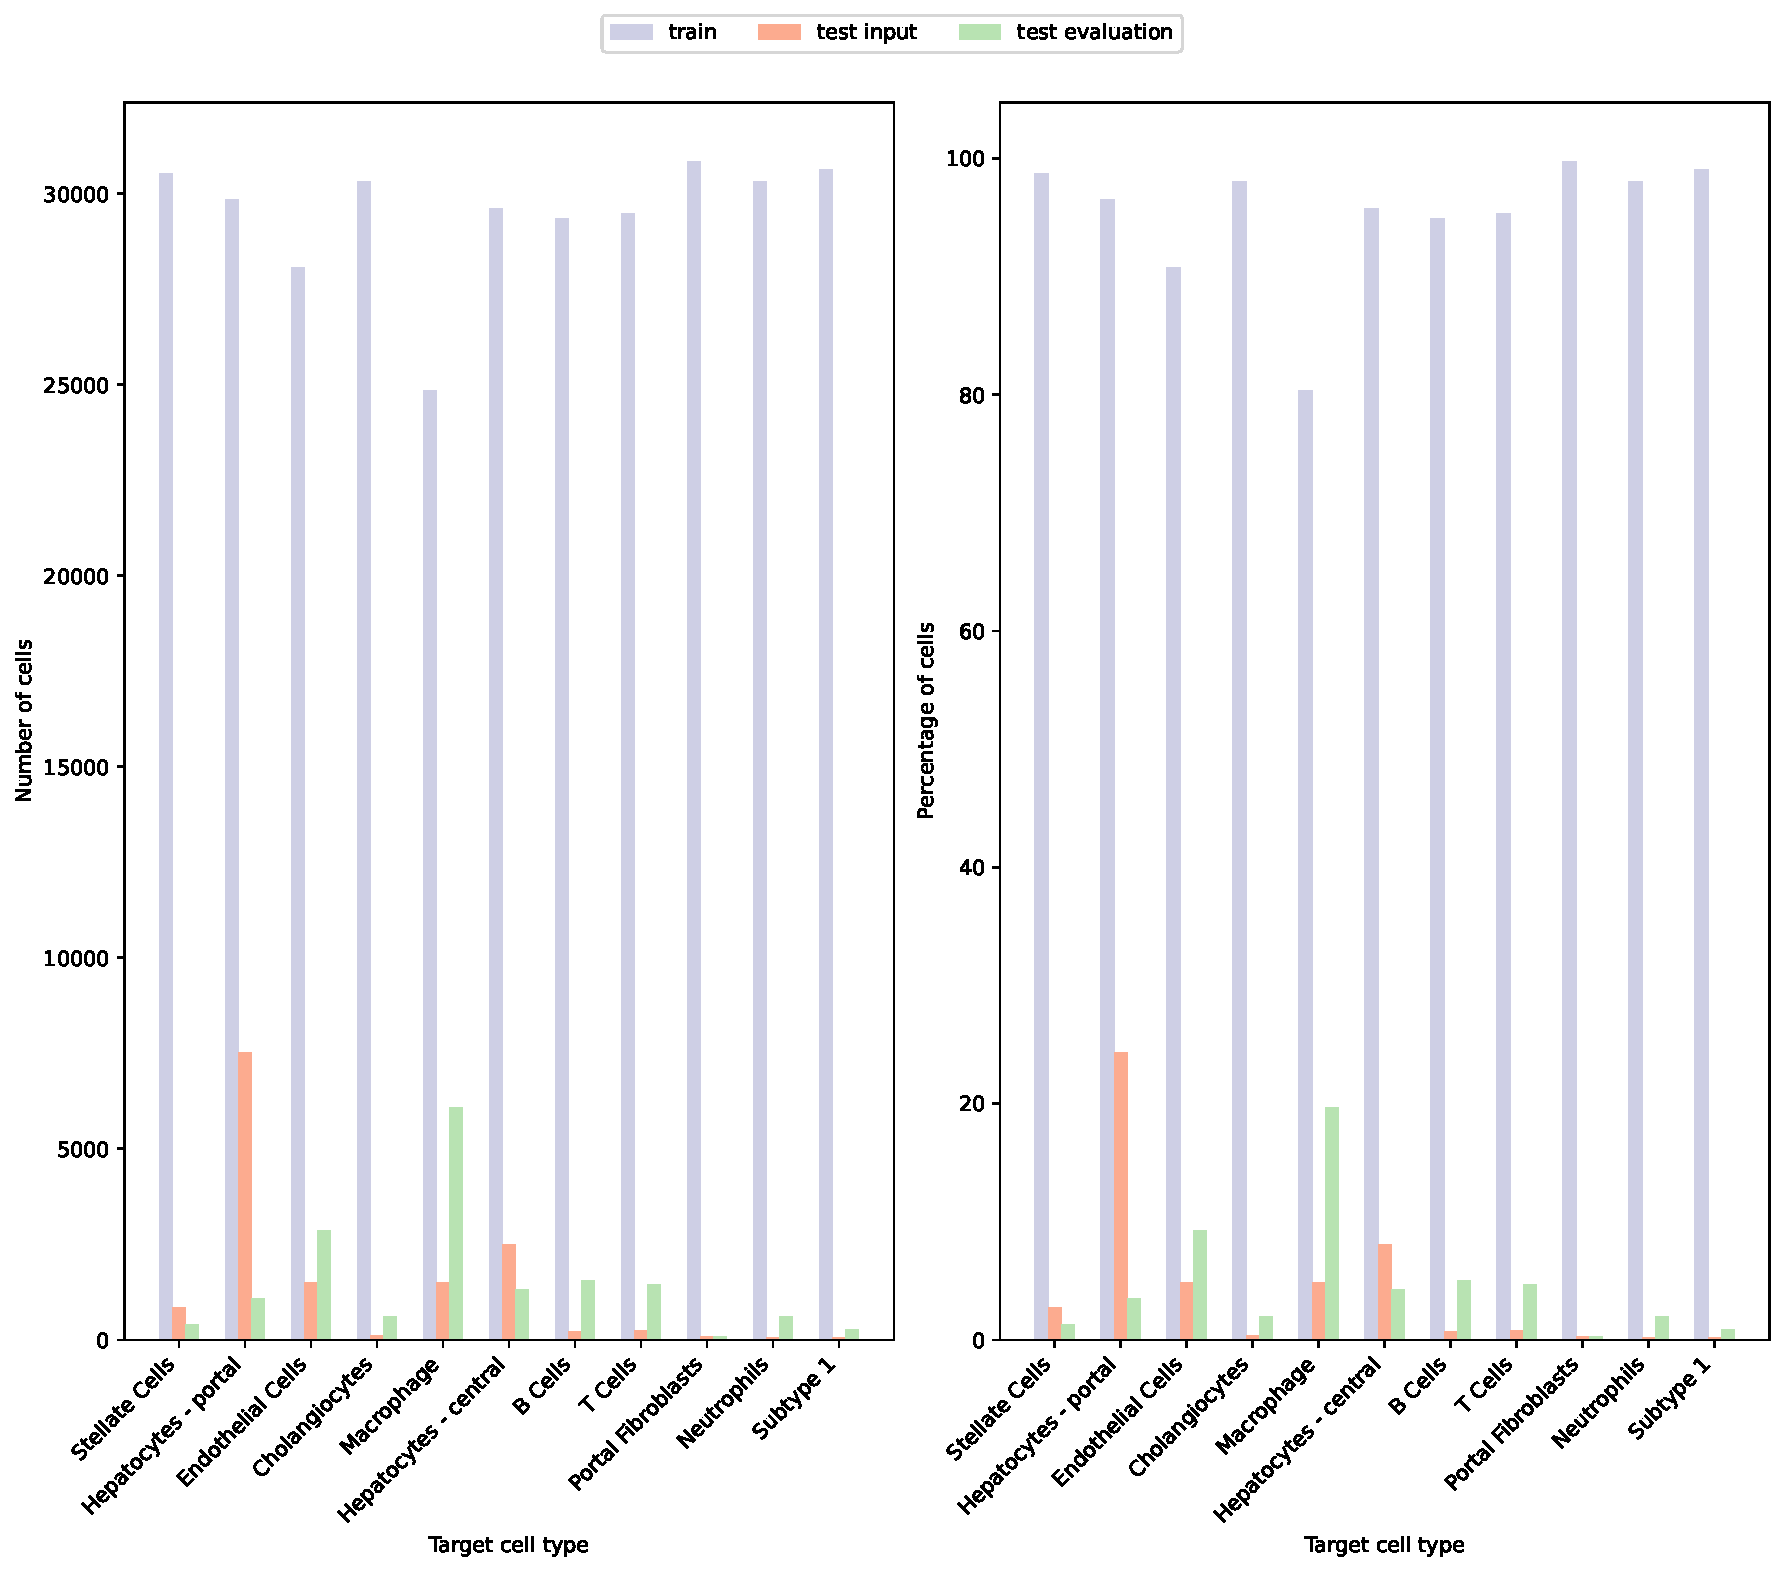
\includegraphics[width=.7\textwidth]{figures/nault_bars_split_30.pdf}
    \caption{Number of cells per cell type for $30 \mu g/kg$}
\end{figure}

\clearpage


\subsection{Comparison}


\begin{figure}[h!]
    \centering
    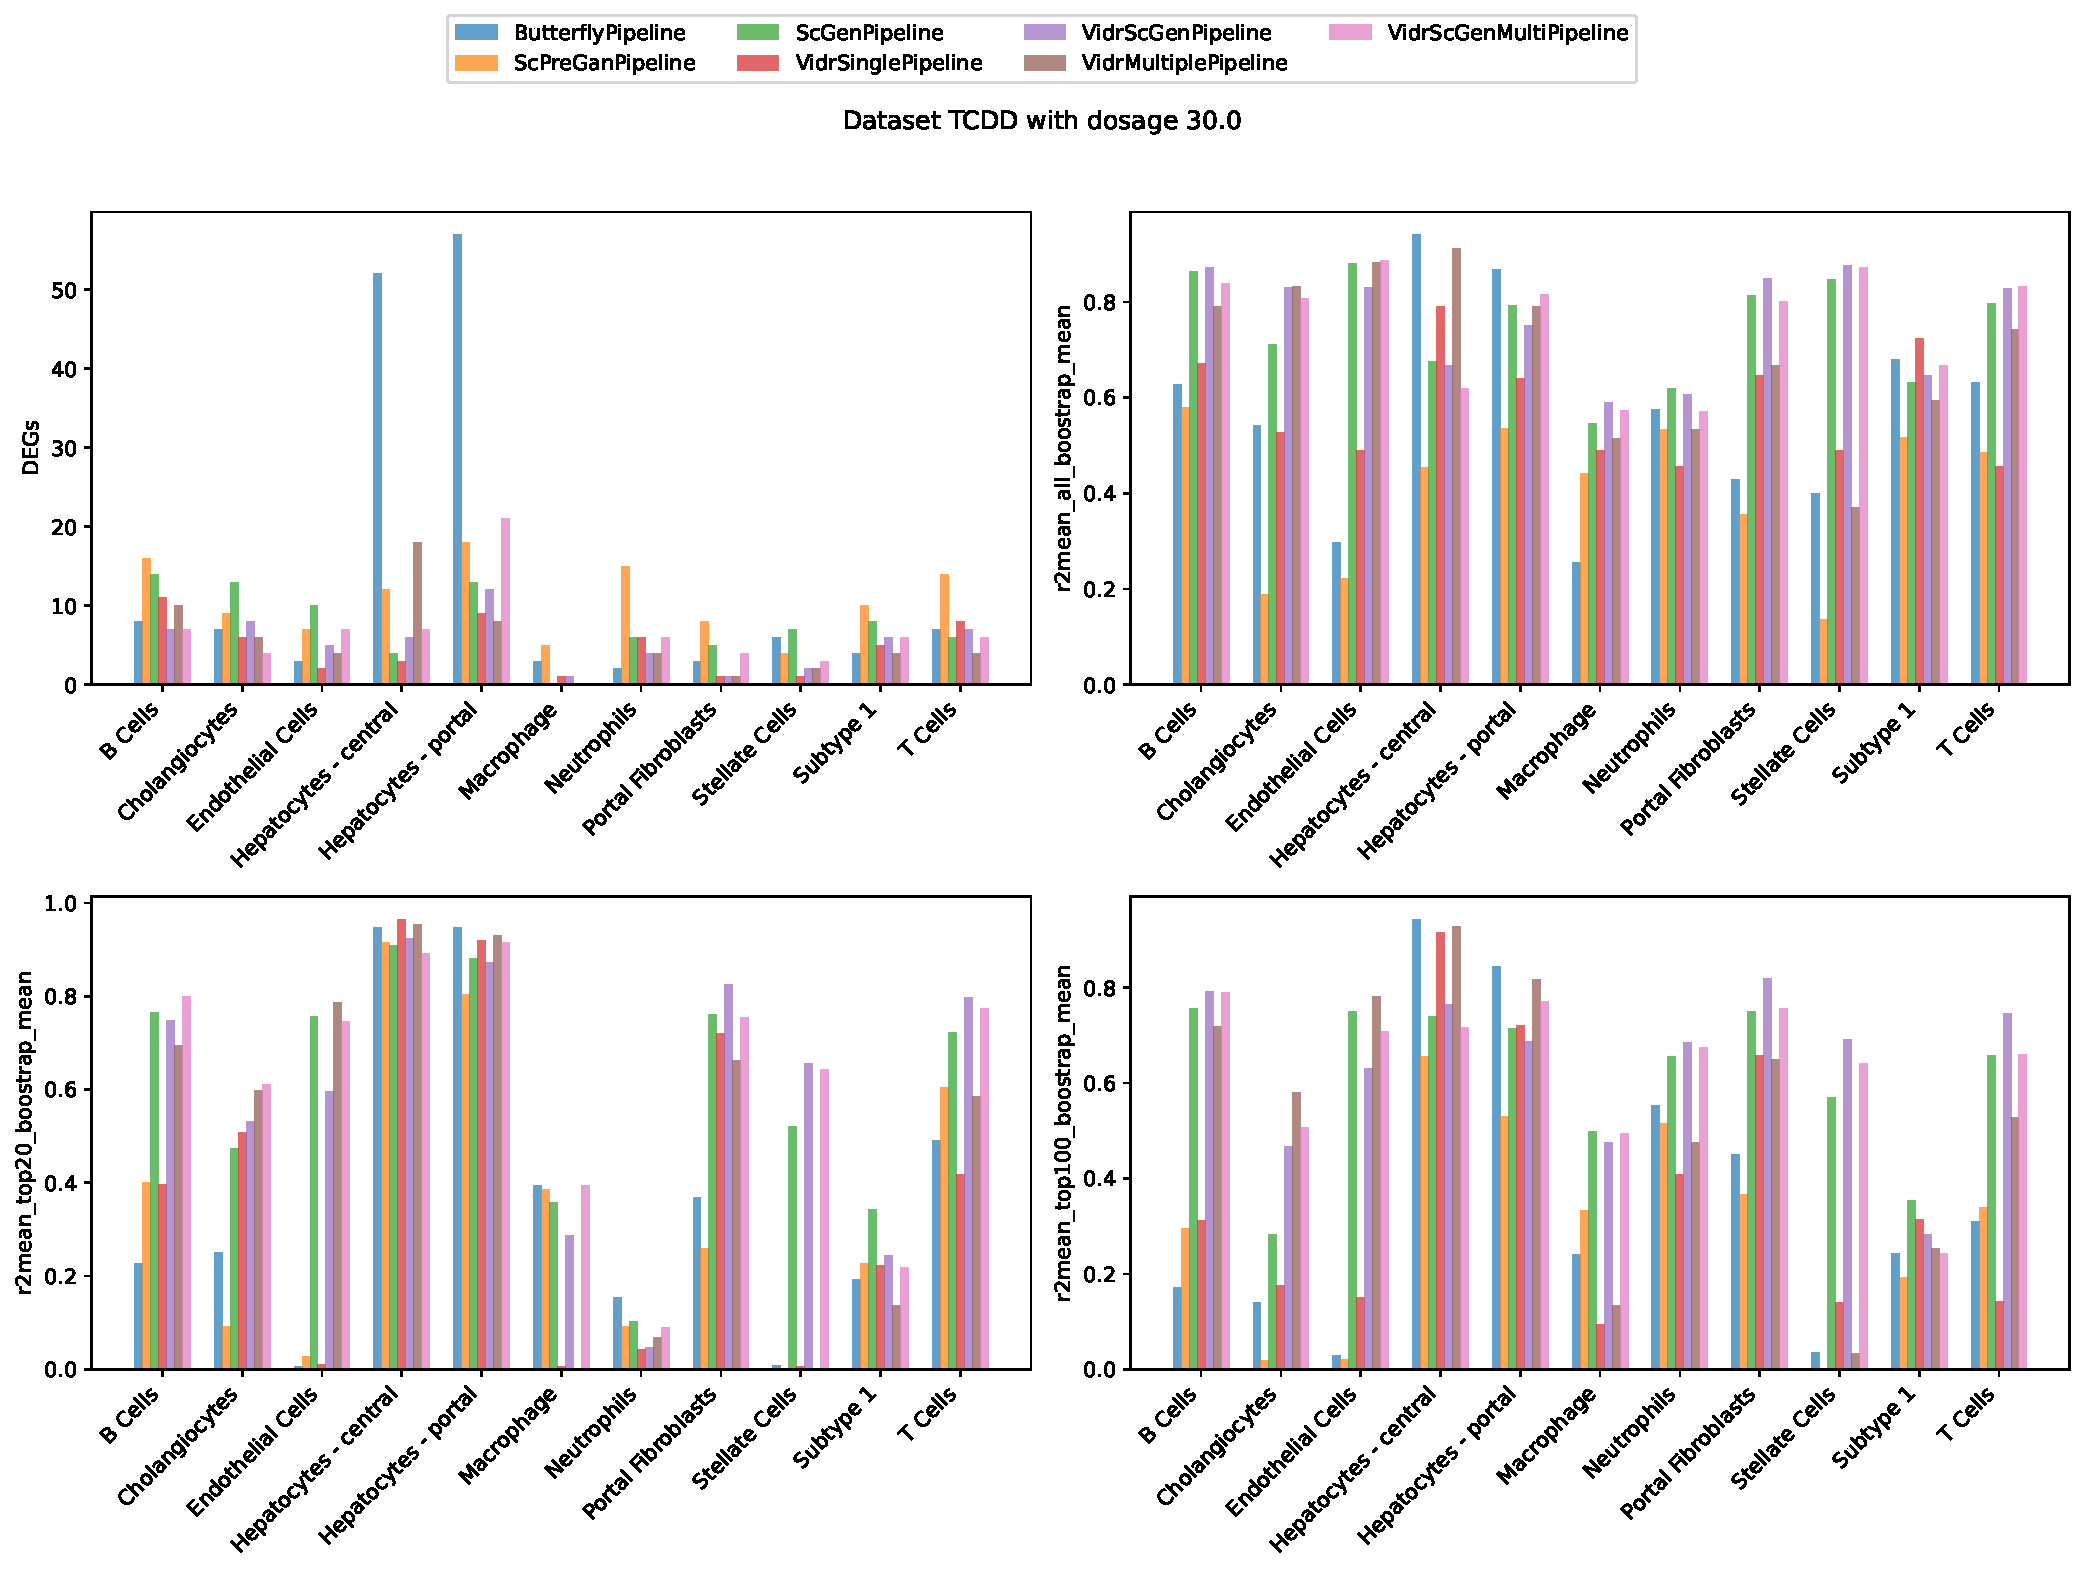
\includegraphics[width=.8\textwidth]{figures/nault_30_baseline_metrics_bars.pdf}
    \caption{Baseline metrics for highest dosage $30 \mu g/kg$ across cell types}
\end{figure}

\begin{figure}[h!]
    \centering
    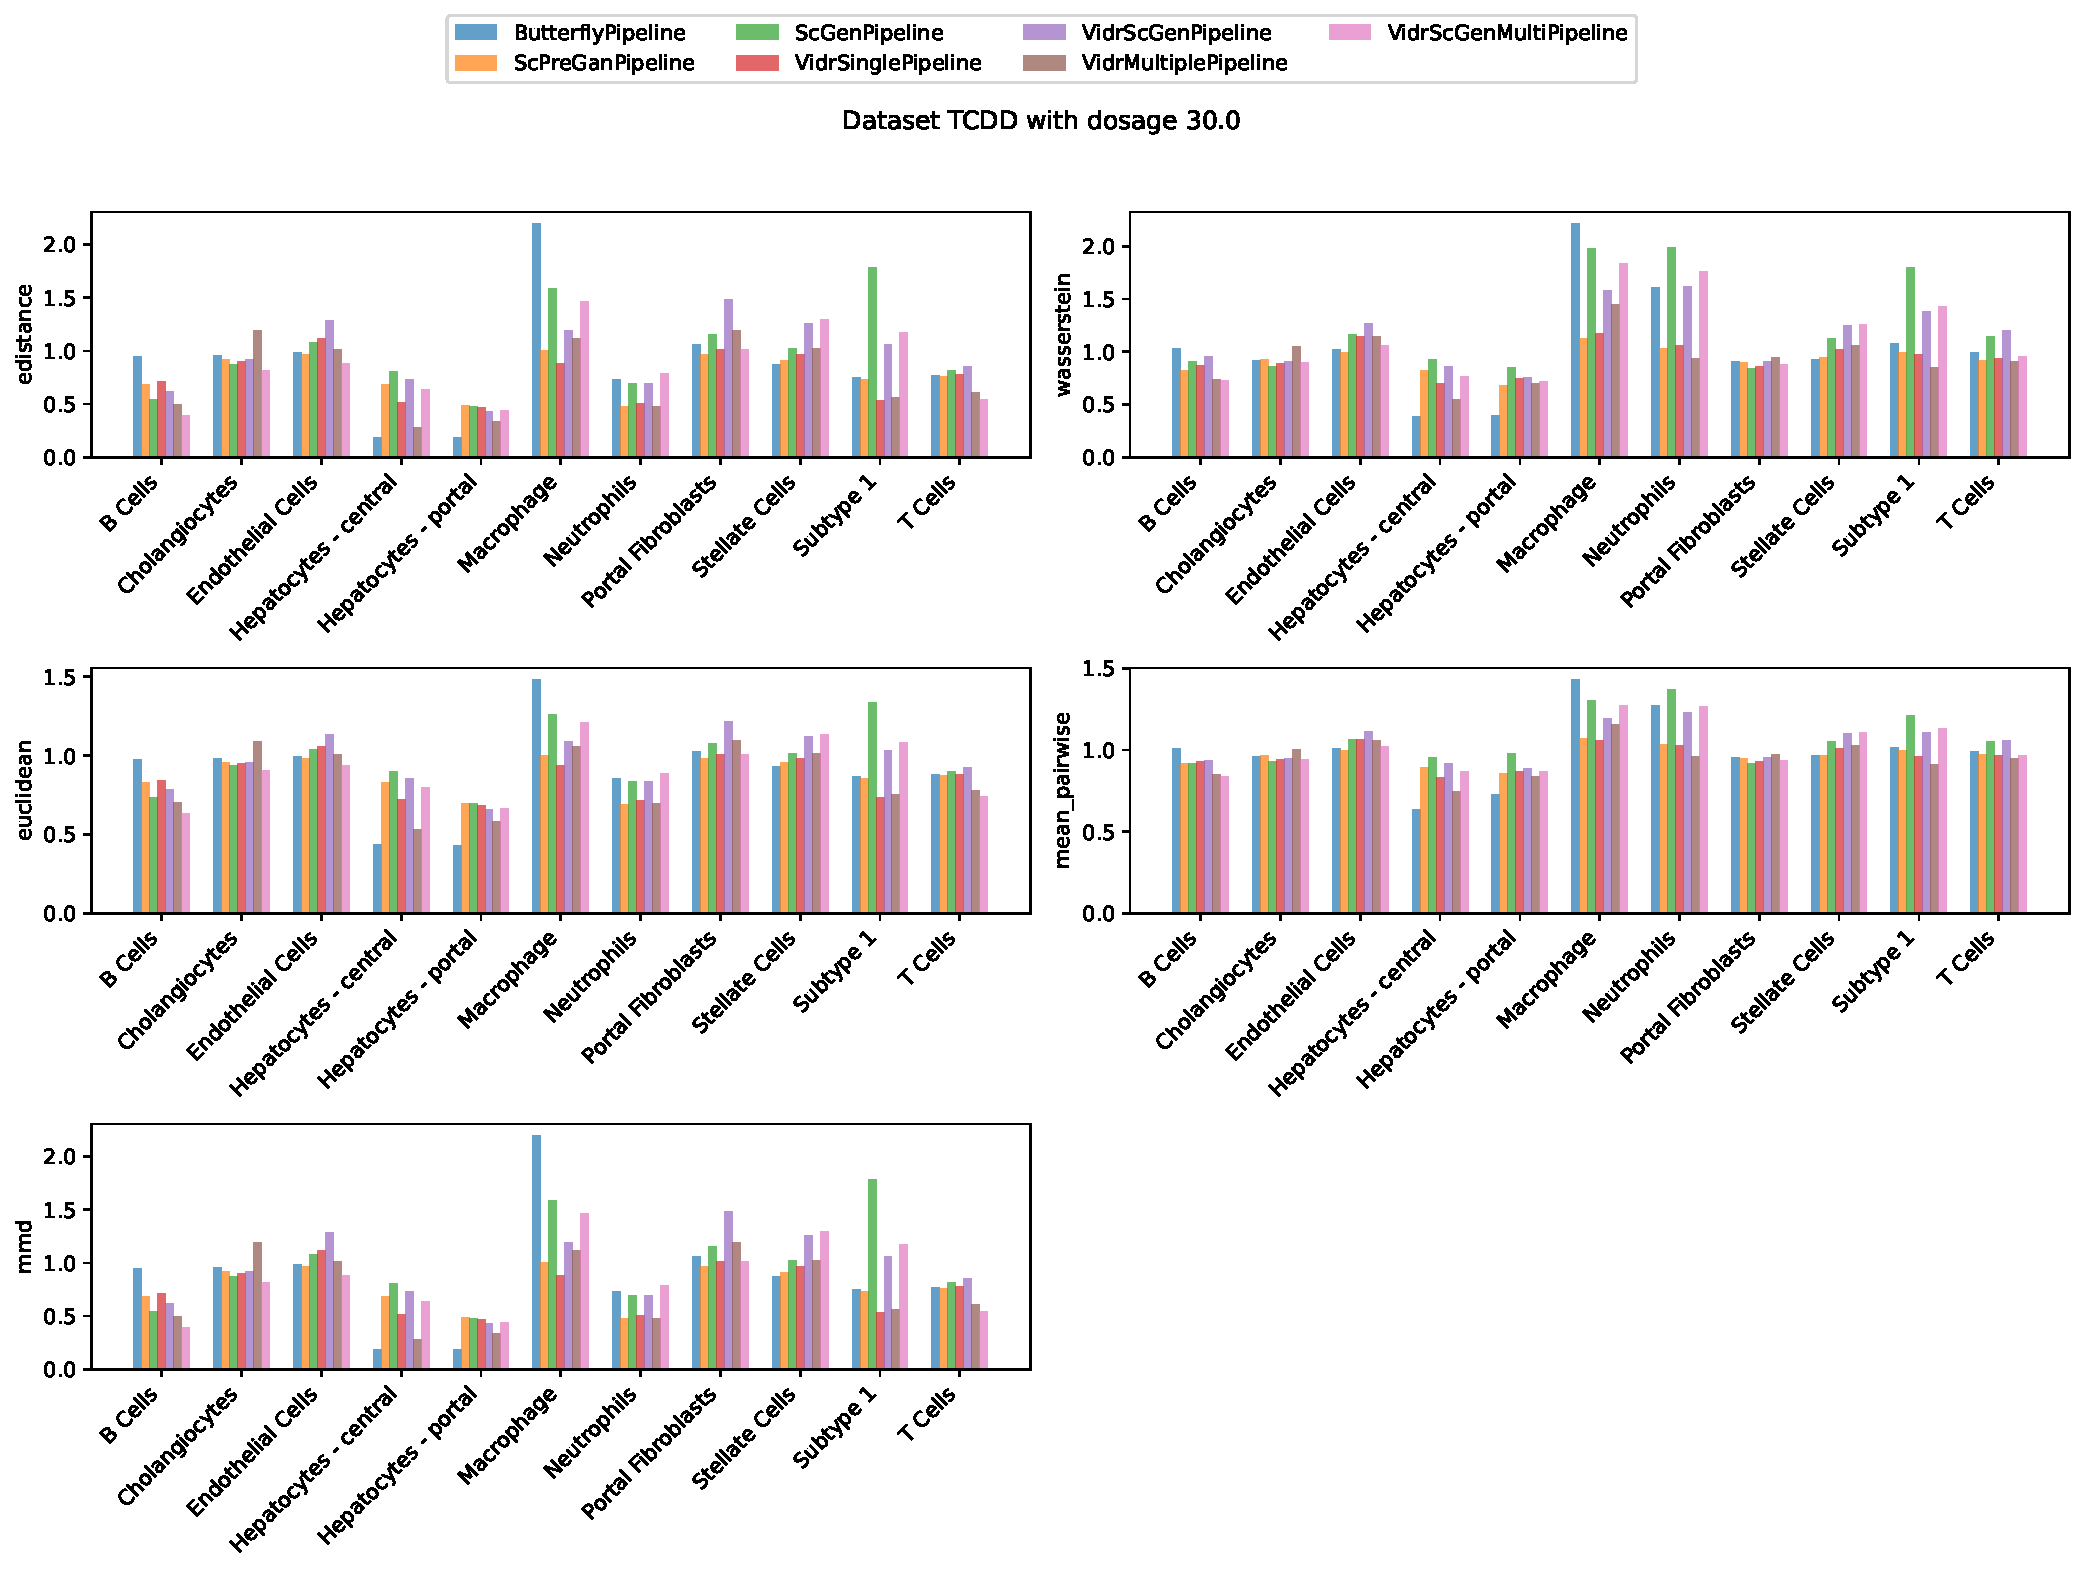
\includegraphics[width=.8\textwidth]{figures/nault_30_distance_metrics_bars.pdf}
    \caption{Distance metrics for highest dosage $30 \mu g/kg$ across cell types}
\end{figure}

\clearpage

\begin{figure}[h!]
    \centering
    \includegraphics[width=.8\textwidth]{figures/nault_01_baseline_metrics_bars.pdf}
    \caption{Baseline metrics for lowest dosage $0.01 \mu g/kg$ across cell types}
\end{figure}

\begin{figure}[h!]
    \centering
    \includegraphics[width=.8\textwidth]{figures/nault_01_distance_metrics_bars.pdf}
    \caption{Distance metrics for lowest dosage $0.01 \mu g/kg$ across cell types}
\end{figure}

\clearpage


\begin{figure}[h!]
    \centering
    \includegraphics[width=.8\textwidth]{figures/nault_hepatocytes_baseline_metrics_bars.pdf}
    \caption{Baseline metrics for Hepatocytes - portal across dosages}
\end{figure}

\begin{figure}[h!]
    \centering
    \includegraphics[width=.8\textwidth]{figures/nault_hepatocytes_distance_metrics_bars.pdf}
    \caption{Distance metrics for Hepatocytes - portal across dosages}
\end{figure}

\clearpage

\begin{figure}
    \centering
    \begin{minipage}{0.49\textwidth}
        \centering
        \includegraphics[width=\textwidth]{figures/3d_nault_DEGs.pdf}
        \caption{}
    \end{minipage} \hfill
    \begin{minipage}{0.49\textwidth}
        \centering
        \includegraphics[width=\textwidth]{figures/3d_nault_r2mean_all_boostrap_mean.pdf}
        \caption{}
    \end{minipage}
    \vskip\baselineskip

    \begin{minipage}{0.49\textwidth}
        \centering
        \includegraphics[width=\textwidth]{figures/3d_nault_r2mean_top20_boostrap_mean.pdf}
        \caption{}
    \end{minipage} \hfill
    \begin{minipage}{0.49\textwidth}
        \centering
        \includegraphics[width=\textwidth]{figures/3d_nault_r2mean_top100_boostrap_mean.pdf}
        \caption{}
    \end{minipage}
    \vskip\baselineskip
\end{figure}

\clearpage

\begin{figure}
    \centering
    \begin{minipage}{0.4\textwidth}
        \centering
        \includegraphics[width=\textwidth]{figures/3d_nault_edistance.pdf}
        \caption{E-distance}
    \end{minipage} \hfill
    \begin{minipage}{0.4\textwidth}
        \centering
        \includegraphics[width=\textwidth]{figures/3d_nault_euclidean.pdf}
        \caption{Euclidean}
    \end{minipage}
    \vskip\baselineskip

    \begin{minipage}{0.4\textwidth}
        \centering
        \includegraphics[width=\textwidth]{figures/3d_nault_mean_pairwise.pdf}
        \caption{Mean pairwise}
    \end{minipage} \hfill
    \begin{minipage}{0.4\textwidth}
        \centering
        \includegraphics[width=\textwidth]{figures/3d_nault_mmd.pdf}
        \caption{MMD}
    \end{minipage}
    \vskip\baselineskip

    \begin{minipage}{0.4\textwidth}
        \centering
        \includegraphics[width=\textwidth]{figures/3d_nault_wasserstein.pdf}
        \caption{Wasserstein}
    \end{minipage}
    \caption{Distance metrics per cell type}
\end{figure}

\clearpage


\begin{figure}[h!]
    \centering
    \includegraphics[width=.9\textwidth]{figures/NaultPipeline_X_Violin_metrics0.pdf}
\end{figure}

\begin{figure}[h!]
    \centering
    \includegraphics[width=.9\textwidth]{figures/NaultPipeline_X_Violin_metrics1.pdf}
\end{figure}

\clearpage

\begin{figure}[h!]
    \centering
    \includegraphics[width=.9\textwidth]{figures/NaultPipeline_X_Boxplot_metrics0.pdf}
\end{figure}

\begin{figure}[h!]
    \centering
    \includegraphics[width=.9\textwidth]{figures/NaultPipeline_X_Boxplot_metrics1.pdf}
\end{figure}

\clearpage

\begin{figure}[h!]
    \centering
    \includegraphics[width=.9\textwidth]{figures/NaultPipeline_Y_Violin_metrics0.pdf}
\end{figure}

\begin{figure}[h!]
    \centering
    \includegraphics[width=.9\textwidth]{figures/NaultPipeline_Y_Violin_metrics1.pdf}
\end{figure}

\clearpage

\begin{figure}[h!]
    \centering
    \includegraphics[width=.9\textwidth]{figures/NaultPipeline_Y_Boxplot_metrics0.pdf}
\end{figure}

\begin{figure}[h!]
    \centering
    \includegraphics[width=.9\textwidth]{figures/NaultPipeline_Y_Boxplot_metrics1.pdf}
\end{figure}

\clearpage

\begin{figure}[h!]
    \centering
    \includegraphics[width=.8\textwidth]{figures/nault_contour_DEGs.pdf}
    \caption{DEGs}
\end{figure}

\begin{figure}[h!]
    \centering
    \includegraphics[width=.8\textwidth]{figures/nault_contour_r2mean_all_boostrap_mean.pdf}
    \caption{r2 HVGs}
\end{figure}

\clearpage

\begin{figure}[h!]
    \centering
    \includegraphics[width=.8\textwidth]{figures/nault_contour_r2mean_top20_boostrap_mean.pdf}
    \caption{r2 top 20}
\end{figure}

\begin{figure}[h!]
    \centering
    \includegraphics[width=.8\textwidth]{figures/nault_contour_r2mean_top100_boostrap_mean.pdf}
    \caption{r2 top 100}
\end{figure}

\clearpage

\begin{figure}[h!]
    \centering
    \includegraphics[width=.8\textwidth]{figures/nault_contour_edistance.pdf}
    \caption{E-distance}
\end{figure}

\begin{figure}[h!]
    \centering
    \includegraphics[width=.8\textwidth]{figures/nault_contour_euclidean.pdf}
    \caption{Euclidean}
\end{figure}

\clearpage

\begin{figure}[h!]
    \centering
    \includegraphics[width=.8\textwidth]{figures/nault_contour_mean_pairwise.pdf}
    \caption{Mean pairwise}
\end{figure}

\begin{figure}[h!]
    \centering
    \includegraphics[width=.8\textwidth]{figures/nault_contour_mmd.pdf}
    \caption{MMD}
\end{figure}

\clearpage

\begin{figure}[h!]
    \centering
    \includegraphics[width=\textwidth]{figures/nault_contour_wasserstein.pdf}
    \caption{Wasserstein}
\end{figure}

\clearpage

\section{Nault liver cell types evaluation}


\subsection{Multiple doses}


\begin{figure}[h!]
    \centering
    \includegraphics[width=.8\textwidth]{figures/nault_liver_umap_split_multiple.png}
\end{figure}

\begin{figure}[h!]
    \centering
    \includegraphics[width=.8\textwidth]{figures/nault_liver_bars_split_multiple.pdf}
\end{figure}


\subsection{Single dose 30 $\mu g/kg$}

\begin{figure}[h!]
    \centering
    \includegraphics[width=.8\textwidth]{figures/nault_liver_umap_split_30.png}
\end{figure}

\begin{figure}[h!]
    \centering
    \includegraphics[width=.8\textwidth]{figures/nault_liver_bars_split_30.pdf}
\end{figure}


\clearpage

\subsection{Comparison}


\begin{figure}[h!]
    \centering
    \includegraphics[width=.8\textwidth]{figures/nault_liver_30_baseline_metrics_bars.pdf}
    \caption{Baseline metrics for highest dosage $30 \mu g/kg$ across cell types}
\end{figure}

\begin{figure}[h!]
    \centering
    \includegraphics[width=.8\textwidth]{figures/nault_liver_30_distance_metrics_bars.pdf}
    \caption{Distance metrics for highest dosage $30 \mu g/kg$ across cell types}
\end{figure}

\clearpage

\begin{figure}[h!]
    \centering
    \includegraphics[width=.8\textwidth]{figures/nault_liver_01_baseline_metrics_bars.pdf}
    \caption{Baseline metrics for highest dosage $0.1 \mu g/kg$ across cell types}
\end{figure}

\begin{figure}[h!]
    \centering
    \includegraphics[width=.8\textwidth]{figures/nault_liver_01_distance_metrics_bars.pdf}
    \caption{Distance metrics for highest dosage $0.1 \mu g/kg$ across cell types}
\end{figure}

\clearpage

\begin{figure}[h!]
    \centering
    \includegraphics[width=.8\textwidth]{figures/nault_liver_hepatocytes_baseline_metrics_bars.pdf}
    \caption{Baseline metrics for Hepatocytes - portal across dosages}
\end{figure}

\begin{figure}[h!]
    \centering
    \includegraphics[width=.8\textwidth]{figures/nault_liver_hepatocytes_distance_metrics_bars.pdf}
    \caption{Distance metrics for Hepatocytes - portal across dosages}
\end{figure}

\clearpage


\begin{figure}
    \centering
    \begin{minipage}{0.49\textwidth}
        \centering
        \includegraphics[width=\textwidth]{figures/3d_nault_liver_DEGs.pdf}
        \caption{}
    \end{minipage} \hfill
    \begin{minipage}{0.49\textwidth}
        \centering
        \includegraphics[width=\textwidth]{figures/3d_nault_liver_r2mean_all_boostrap_mean.pdf}
        \caption{}
    \end{minipage}
    \vskip\baselineskip

    \begin{minipage}{0.49\textwidth}
        \centering
        \includegraphics[width=\textwidth]{figures/3d_nault_liver_r2mean_top20_boostrap_mean.pdf}
        \caption{}
    \end{minipage} \hfill
    \begin{minipage}{0.49\textwidth}
        \centering
        \includegraphics[width=\textwidth]{figures/3d_nault_liver_r2mean_top100_boostrap_mean.pdf}
        \caption{}
    \end{minipage}
    \vskip\baselineskip
\end{figure}

\clearpage

\begin{figure}
    \centering
    \begin{minipage}{0.4\textwidth}
        \centering
        \includegraphics[width=\textwidth]{figures/3d_nault_liver_edistance.pdf}
        \caption{E-distance}
    \end{minipage} \hfill
    \begin{minipage}{0.4\textwidth}
        \centering
        \includegraphics[width=\textwidth]{figures/3d_nault_liver_euclidean.pdf}
        \caption{Euclidean}
    \end{minipage}
    \vskip\baselineskip

    \begin{minipage}{0.4\textwidth}
        \centering
        \includegraphics[width=\textwidth]{figures/3d_nault_liver_mean_pairwise.pdf}
        \caption{Mean pairwise}
    \end{minipage} \hfill
    \begin{minipage}{0.4\textwidth}
        \centering
        \includegraphics[width=\textwidth]{figures/3d_nault_liver_mmd.pdf}
        \caption{MMD}
    \end{minipage}
    \vskip\baselineskip

    \begin{minipage}{0.4\textwidth}
        \centering
        \includegraphics[width=\textwidth]{figures/3d_nault_liver_wasserstein.pdf}
        \caption{Wasserstein}
    \end{minipage}
    \caption{Distance metrics per cell type}
\end{figure}

\clearpage


\begin{figure}[h!]
    \centering
    \includegraphics[width=.9\textwidth]{figures/NaultLiverPipeline_X_Violin_metrics0.pdf}
\end{figure}

\begin{figure}[h!]
    \centering
    \includegraphics[width=.9\textwidth]{figures/NaultLiverPipeline_X_Violin_metrics1.pdf}
\end{figure}

\clearpage

\begin{figure}[h!]
    \centering
    \includegraphics[width=.9\textwidth]{figures/NaultLiverPipeline_X_Boxplot_metrics0.pdf}
\end{figure}

\begin{figure}[h!]
    \centering
    \includegraphics[width=.9\textwidth]{figures/NaultLiverPipeline_X_Boxplot_metrics1.pdf}
\end{figure}

\clearpage

\begin{figure}[h!]
    \centering
    \includegraphics[width=.9\textwidth]{figures/NaultLiverPipeline_Y_Violin_metrics0.pdf}
\end{figure}

\begin{figure}[h!]
    \centering
    \includegraphics[width=.9\textwidth]{figures/NaultLiverPipeline_Y_Violin_metrics1.pdf}
\end{figure}

\clearpage

\begin{figure}[h!]
    \centering
    \includegraphics[width=.9\textwidth]{figures/NaultLiverPipeline_Y_Boxplot_metrics0.pdf}
\end{figure}

\begin{figure}[h!]
    \centering
    \includegraphics[width=.9\textwidth]{figures/NaultLiverPipeline_Y_Boxplot_metrics1.pdf}
\end{figure}

\clearpage

\begin{figure}[h!]
    \centering
    \includegraphics[width=.8\textwidth]{figures/nault_liver_contour_DEGs.pdf}
    \caption{DEGs}
\end{figure}

\begin{figure}[h!]
    \centering
    \includegraphics[width=.8\textwidth]{figures/nault_liver_contour_r2mean_all_boostrap_mean.pdf}
    \caption{r2 HVGs}
\end{figure}

\clearpage

\begin{figure}[h!]
    \centering
    \includegraphics[width=.8\textwidth]{figures/nault_liver_contour_r2mean_top20_boostrap_mean.pdf}
    \caption{r2 top 20}
\end{figure}

\begin{figure}[h!]
    \centering
    \includegraphics[width=.8\textwidth]{figures/nault_liver_contour_r2mean_top100_boostrap_mean.pdf}
    \caption{r2 top 100}
\end{figure}

\clearpage

\begin{figure}[h!]
    \centering
    \includegraphics[width=.8\textwidth]{figures/nault_liver_contour_edistance.pdf}
    \caption{E-distance}
\end{figure}

\begin{figure}[h!]
    \centering
    \includegraphics[width=.8\textwidth]{figures/nault_liver_contour_euclidean.pdf}
\end{figure}

\clearpage

\begin{figure}[h!]
    \centering
    \includegraphics[width=.8\textwidth]{figures/nault_liver_contour_mean_pairwise.pdf}
    \caption{Mean pairwise}
\end{figure}

\begin{figure}[h!]
    \centering
    \includegraphics[width=.8\textwidth]{figures/nault_liver_contour_mmd.pdf}
    \caption{MMD}
\end{figure}

\clearpage

\begin{figure}[h!]
    \centering
    \includegraphics[width=\textwidth]{figures/nault_liver_contour_wasserstein.pdf}
    \caption{Wasserstein}
\end{figure}

\clearpage

\subsection{Παρατηρήσεις}

\begin{itemize}
    \itemsep -0.2em
    \item Το scButterfly και το scPreGan έχουν παρόμοια συμπεριφορά στις μετρικές και εμφανίζουν μεγάλη διακύμανση κατά μήκος των τύπων των κυττάρων και των δόσεων.
    \item Τα μοντέλα που έχουν ως βάση την αρχιτεκτονική του scGen (scVIDR, και οι παραλλαγές του), VAR και post-processing στο latent space, έχουν την υψηλότερη και πιο σταθερή απόδοση σε μετρικές του $R^2$, ωστόσο υστερούν στην καταμέτρηση των κοινών διαφοροποιήσιμων γονιδίων έκφρασης (DEGs).
\end{itemize}

\clearpage

\section{PBMC}


\begin{figure}[h!]
    \centering
    \includegraphics[width=.8\textwidth]{figures/pbmc_split.png}
\end{figure}

\begin{figure}[h!]
    \centering
    \includegraphics[width=.8\textwidth]{figures/pbmc_bars_split.pdf}
\end{figure}

\clearpage

\subsection{Comparison}

\begin{figure}[h!]
    \centering
    \includegraphics[width=.8\textwidth]{figures/pbmc_baseline_metrics_bars.pdf}
\end{figure}

\begin{figure}[h!]
    \centering
    \includegraphics[width=.8\textwidth]{figures/pbmc_distance_metrics_bars.pdf}
\end{figure}

\appendix
\chapter{Ακρωνύμια και συντομογραφίες}

\begin{description}
  \item[LAN] Local Area Network
\end{description}



\bibliographystyle{plain}
\bibliography{references.bib}

\end{document}